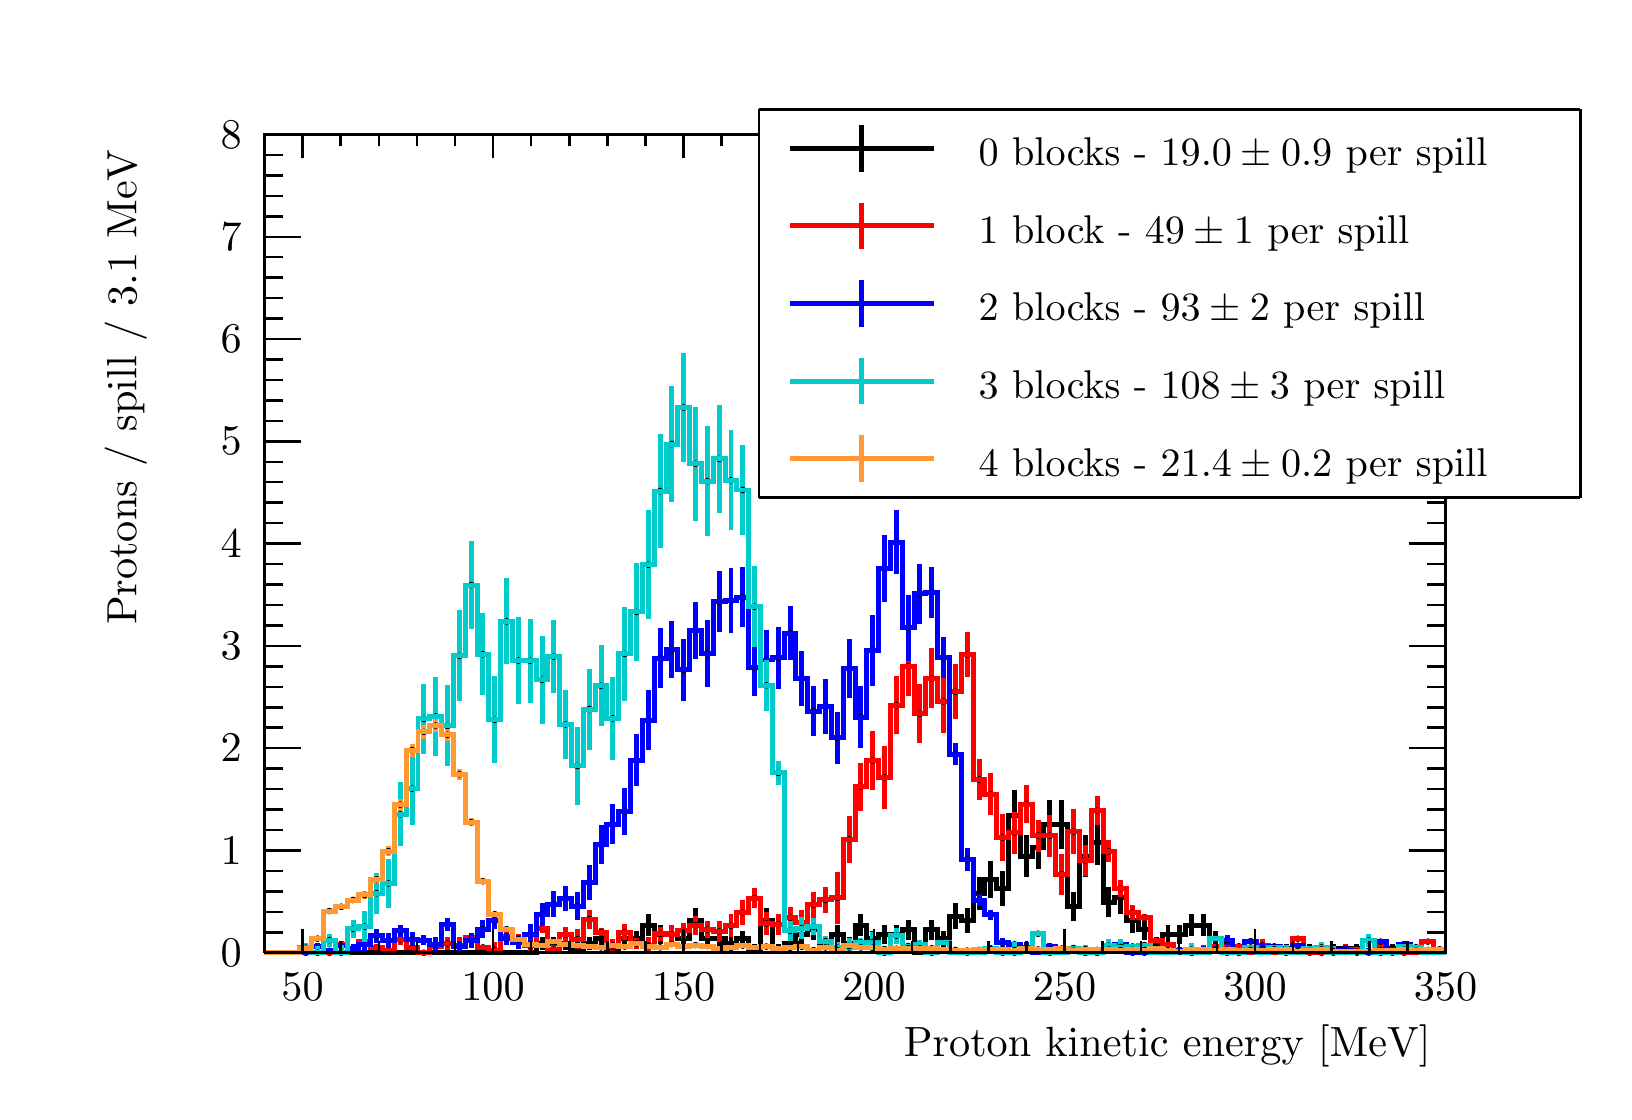
\begin{tikzpicture}
\pgfdeclareplotmark{cross} {
\pgfpathmoveto{\pgfpoint{-0.3\pgfplotmarksize}{\pgfplotmarksize}}
\pgfpathlineto{\pgfpoint{+0.3\pgfplotmarksize}{\pgfplotmarksize}}
\pgfpathlineto{\pgfpoint{+0.3\pgfplotmarksize}{0.3\pgfplotmarksize}}
\pgfpathlineto{\pgfpoint{+1\pgfplotmarksize}{0.3\pgfplotmarksize}}
\pgfpathlineto{\pgfpoint{+1\pgfplotmarksize}{-0.3\pgfplotmarksize}}
\pgfpathlineto{\pgfpoint{+0.3\pgfplotmarksize}{-0.3\pgfplotmarksize}}
\pgfpathlineto{\pgfpoint{+0.3\pgfplotmarksize}{-1.\pgfplotmarksize}}
\pgfpathlineto{\pgfpoint{-0.3\pgfplotmarksize}{-1.\pgfplotmarksize}}
\pgfpathlineto{\pgfpoint{-0.3\pgfplotmarksize}{-0.3\pgfplotmarksize}}
\pgfpathlineto{\pgfpoint{-1.\pgfplotmarksize}{-0.3\pgfplotmarksize}}
\pgfpathlineto{\pgfpoint{-1.\pgfplotmarksize}{0.3\pgfplotmarksize}}
\pgfpathlineto{\pgfpoint{-0.3\pgfplotmarksize}{0.3\pgfplotmarksize}}
\pgfpathclose
\pgfusepathqstroke
}
\pgfdeclareplotmark{cross*} {
\pgfpathmoveto{\pgfpoint{-0.3\pgfplotmarksize}{\pgfplotmarksize}}
\pgfpathlineto{\pgfpoint{+0.3\pgfplotmarksize}{\pgfplotmarksize}}
\pgfpathlineto{\pgfpoint{+0.3\pgfplotmarksize}{0.3\pgfplotmarksize}}
\pgfpathlineto{\pgfpoint{+1\pgfplotmarksize}{0.3\pgfplotmarksize}}
\pgfpathlineto{\pgfpoint{+1\pgfplotmarksize}{-0.3\pgfplotmarksize}}
\pgfpathlineto{\pgfpoint{+0.3\pgfplotmarksize}{-0.3\pgfplotmarksize}}
\pgfpathlineto{\pgfpoint{+0.3\pgfplotmarksize}{-1.\pgfplotmarksize}}
\pgfpathlineto{\pgfpoint{-0.3\pgfplotmarksize}{-1.\pgfplotmarksize}}
\pgfpathlineto{\pgfpoint{-0.3\pgfplotmarksize}{-0.3\pgfplotmarksize}}
\pgfpathlineto{\pgfpoint{-1.\pgfplotmarksize}{-0.3\pgfplotmarksize}}
\pgfpathlineto{\pgfpoint{-1.\pgfplotmarksize}{0.3\pgfplotmarksize}}
\pgfpathlineto{\pgfpoint{-0.3\pgfplotmarksize}{0.3\pgfplotmarksize}}
\pgfpathclose
\pgfusepathqfillstroke
}
\pgfdeclareplotmark{newstar} {
\pgfpathmoveto{\pgfqpoint{0pt}{\pgfplotmarksize}}
\pgfpathlineto{\pgfqpointpolar{44}{0.5\pgfplotmarksize}}
\pgfpathlineto{\pgfqpointpolar{18}{\pgfplotmarksize}}
\pgfpathlineto{\pgfqpointpolar{-20}{0.5\pgfplotmarksize}}
\pgfpathlineto{\pgfqpointpolar{-54}{\pgfplotmarksize}}
\pgfpathlineto{\pgfqpointpolar{-90}{0.5\pgfplotmarksize}}
\pgfpathlineto{\pgfqpointpolar{234}{\pgfplotmarksize}}
\pgfpathlineto{\pgfqpointpolar{198}{0.5\pgfplotmarksize}}
\pgfpathlineto{\pgfqpointpolar{162}{\pgfplotmarksize}}
\pgfpathlineto{\pgfqpointpolar{134}{0.5\pgfplotmarksize}}
\pgfpathclose
\pgfusepathqstroke
}
\pgfdeclareplotmark{newstar*} {
\pgfpathmoveto{\pgfqpoint{0pt}{\pgfplotmarksize}}
\pgfpathlineto{\pgfqpointpolar{44}{0.5\pgfplotmarksize}}
\pgfpathlineto{\pgfqpointpolar{18}{\pgfplotmarksize}}
\pgfpathlineto{\pgfqpointpolar{-20}{0.5\pgfplotmarksize}}
\pgfpathlineto{\pgfqpointpolar{-54}{\pgfplotmarksize}}
\pgfpathlineto{\pgfqpointpolar{-90}{0.5\pgfplotmarksize}}
\pgfpathlineto{\pgfqpointpolar{234}{\pgfplotmarksize}}
\pgfpathlineto{\pgfqpointpolar{198}{0.5\pgfplotmarksize}}
\pgfpathlineto{\pgfqpointpolar{162}{\pgfplotmarksize}}
\pgfpathlineto{\pgfqpointpolar{134}{0.5\pgfplotmarksize}}
\pgfpathclose
\pgfusepathqfillstroke
}
\definecolor{c}{rgb}{1,1,1};
\draw [color=c, fill=c] (0,0) rectangle (20,13.4957);
\draw [color=c, fill=c] (3,1.75444) rectangle (18,12.1461);
\definecolor{c}{rgb}{0,0,0};
\draw [c,line width=0.9] (3,1.75444) -- (3,12.1461) -- (18,12.1461) -- (18,1.75444) -- (3,1.75444);
\definecolor{c}{rgb}{1,1,1};
\draw [color=c, fill=c] (3,1.75444) rectangle (18,12.1461);
\definecolor{c}{rgb}{0,0,0};
\draw [c,line width=0.9] (3,1.75444) -- (3,12.1461) -- (18,12.1461) -- (18,1.75444) -- (3,1.75444);
\draw [c,line width=0.9] (3,1.75444) -- (3.15,1.75444) -- (3.15,1.75444) -- (3.3,1.75444) -- (3.3,1.75444) -- (3.45,1.75444) -- (3.45,1.75444) -- (3.6,1.75444) -- (3.6,1.75444) -- (3.75,1.75444) -- (3.75,1.75444) -- (3.9,1.75444) -- (3.9,1.75444) --
 (4.05,1.75444) -- (4.05,1.75444) -- (4.2,1.75444) -- (4.2,1.75444) -- (4.35,1.75444) -- (4.35,1.75444) -- (4.5,1.75444) -- (4.5,1.75444) -- (4.65,1.75444) -- (4.65,1.75444) -- (4.8,1.75444) -- (4.8,1.75444) -- (4.95,1.75444) -- (4.95,1.75444) --
 (5.1,1.75444) -- (5.1,1.75444) -- (5.25,1.75444) -- (5.25,1.75444) -- (5.4,1.75444) -- (5.4,1.75444) -- (5.55,1.75444) -- (5.55,1.75444) -- (5.7,1.75444) -- (5.7,1.75444) -- (5.85,1.75444) -- (5.85,1.75444) -- (6,1.75444) -- (6,1.75444) --
 (6.15,1.75444) -- (6.15,1.75444) -- (6.3,1.75444) -- (6.3,1.75444) -- (6.45,1.75444) -- (6.45,1.75444) -- (6.6,1.75444) -- (6.6,1.75444) -- (6.75,1.75444) -- (6.75,1.75444) -- (6.9,1.75444) -- (6.9,1.75444) -- (7.05,1.75444) -- (7.05,1.75444) --
 (7.2,1.75444) -- (7.2,1.75444) -- (7.35,1.75444) -- (7.35,1.75444) -- (7.5,1.75444) -- (7.5,1.75444) -- (7.65,1.75444) -- (7.65,1.75444) -- (7.8,1.75444) -- (7.8,1.75444) -- (7.95,1.75444) -- (7.95,1.75444) -- (8.1,1.75444) -- (8.1,1.75444) --
 (8.25,1.75444) -- (8.25,1.75444) -- (8.4,1.75444) -- (8.4,1.75444) -- (8.55,1.75444) -- (8.55,1.75444) -- (8.7,1.75444) -- (8.7,1.75444) -- (8.85,1.75444) -- (8.85,1.75444) -- (9,1.75444) -- (9,1.75444) -- (9.15,1.75444) -- (9.15,1.75444) --
 (9.3,1.75444) -- (9.3,1.75444) -- (9.45,1.75444) -- (9.45,1.75444) -- (9.6,1.75444) -- (9.6,1.75444) -- (9.75,1.75444) -- (9.75,1.75444) -- (9.9,1.75444) -- (9.9,1.75444) -- (10.05,1.75444) -- (10.05,1.75444) -- (10.2,1.75444) -- (10.2,1.75444) --
 (10.35,1.75444) -- (10.35,1.75444) -- (10.5,1.75444) -- (10.5,1.75444) -- (10.65,1.75444) -- (10.65,1.75444) -- (10.8,1.75444) -- (10.8,1.75444) -- (10.95,1.75444) -- (10.95,1.75444) -- (11.1,1.75444) -- (11.1,1.75444) -- (11.25,1.75444) --
 (11.25,1.75444) -- (11.4,1.75444) -- (11.4,1.75444) -- (11.55,1.75444) -- (11.55,1.75444) -- (11.7,1.75444) -- (11.7,1.75444) -- (11.85,1.75444) -- (11.85,1.75444) -- (12,1.75444) -- (12,1.75444) -- (12.15,1.75444) -- (12.15,1.75444) --
 (12.3,1.75444) -- (12.3,1.75444) -- (12.45,1.75444) -- (12.45,1.75444) -- (12.6,1.75444) -- (12.6,1.75444) -- (12.75,1.75444) -- (12.75,1.75444) -- (12.9,1.75444) -- (12.9,1.75444) -- (13.05,1.75444) -- (13.05,1.75444) -- (13.2,1.75444) --
 (13.2,1.75444) -- (13.35,1.75444) -- (13.35,1.75444) -- (13.5,1.75444) -- (13.5,1.75444) -- (13.65,1.75444) -- (13.65,1.75444) -- (13.8,1.75444) -- (13.8,1.75444) -- (13.95,1.75444) -- (13.95,1.75444) -- (14.1,1.75444) -- (14.1,1.75444) --
 (14.25,1.75444) -- (14.25,1.75444) -- (14.4,1.75444) -- (14.4,1.75444) -- (14.55,1.75444) -- (14.55,1.75444) -- (14.7,1.75444) -- (14.7,1.75444) -- (14.85,1.75444) -- (14.85,1.75444) -- (15,1.75444) -- (15,1.75444) -- (15.15,1.75444) --
 (15.15,1.75444) -- (15.3,1.75444) -- (15.3,1.75444) -- (15.45,1.75444) -- (15.45,1.75444) -- (15.6,1.75444) -- (15.6,1.75444) -- (15.75,1.75444) -- (15.75,1.75444) -- (15.9,1.75444) -- (15.9,1.75444) -- (16.05,1.75444) -- (16.05,1.75444) --
 (16.2,1.75444) -- (16.2,1.75444) -- (16.35,1.75444) -- (16.35,1.75444) -- (16.5,1.75444) -- (16.5,1.75444) -- (16.65,1.75444) -- (16.65,1.75444) -- (16.8,1.75444) -- (16.8,1.75444) -- (16.95,1.75444) -- (16.95,1.75444) -- (17.1,1.75444) --
 (17.1,1.75444) -- (17.25,1.75444) -- (17.25,1.75444) -- (17.4,1.75444) -- (17.4,1.75444) -- (17.55,1.75444) -- (17.55,1.75444) -- (17.7,1.75444) -- (17.7,1.75444) -- (17.85,1.75444) -- (17.85,1.75444) -- (18,1.75444);
\draw [c,line width=0.9] (3,1.75444) -- (18,1.75444);
\draw [c,line width=0.9] (3.48387,2.05809) -- (3.48387,1.75444);
\draw [c,line width=0.9] (3.96774,1.90627) -- (3.96774,1.75444);
\draw [c,line width=0.9] (4.45161,1.90627) -- (4.45161,1.75444);
\draw [c,line width=0.9] (4.93548,1.90627) -- (4.93548,1.75444);
\draw [c,line width=0.9] (5.41935,1.90627) -- (5.41935,1.75444);
\draw [c,line width=0.9] (5.90323,2.05809) -- (5.90323,1.75444);
\draw [c,line width=0.9] (6.3871,1.90627) -- (6.3871,1.75444);
\draw [c,line width=0.9] (6.87097,1.90627) -- (6.87097,1.75444);
\draw [c,line width=0.9] (7.35484,1.90627) -- (7.35484,1.75444);
\draw [c,line width=0.9] (7.83871,1.90627) -- (7.83871,1.75444);
\draw [c,line width=0.9] (8.32258,2.05809) -- (8.32258,1.75444);
\draw [c,line width=0.9] (8.80645,1.90627) -- (8.80645,1.75444);
\draw [c,line width=0.9] (9.29032,1.90627) -- (9.29032,1.75444);
\draw [c,line width=0.9] (9.77419,1.90627) -- (9.77419,1.75444);
\draw [c,line width=0.9] (10.2581,1.90627) -- (10.2581,1.75444);
\draw [c,line width=0.9] (10.7419,2.05809) -- (10.7419,1.75444);
\draw [c,line width=0.9] (11.2258,1.90627) -- (11.2258,1.75444);
\draw [c,line width=0.9] (11.7097,1.90627) -- (11.7097,1.75444);
\draw [c,line width=0.9] (12.1935,1.90627) -- (12.1935,1.75444);
\draw [c,line width=0.9] (12.6774,1.90627) -- (12.6774,1.75444);
\draw [c,line width=0.9] (13.1613,2.05809) -- (13.1613,1.75444);
\draw [c,line width=0.9] (13.6452,1.90627) -- (13.6452,1.75444);
\draw [c,line width=0.9] (14.129,1.90627) -- (14.129,1.75444);
\draw [c,line width=0.9] (14.6129,1.90627) -- (14.6129,1.75444);
\draw [c,line width=0.9] (15.0968,1.90627) -- (15.0968,1.75444);
\draw [c,line width=0.9] (15.5806,2.05809) -- (15.5806,1.75444);
\draw [c,line width=0.9] (16.0645,1.90627) -- (16.0645,1.75444);
\draw [c,line width=0.9] (16.5484,1.90627) -- (16.5484,1.75444);
\draw [c,line width=0.9] (17.0323,1.90627) -- (17.0323,1.75444);
\draw [c,line width=0.9] (17.5161,1.90627) -- (17.5161,1.75444);
\draw [c,line width=0.9] (18,2.05809) -- (18,1.75444);
\draw [c,line width=0.9] (3.48387,2.05809) -- (3.48387,1.75444);
\draw [c,line width=0.9] (18,2.05809) -- (18,1.75444);
\draw [anchor=base] (3.48387,1.14713) node[scale=1.52731, color=c, rotate=0]{50};
\draw [anchor=base] (5.90323,1.14713) node[scale=1.52731, color=c, rotate=0]{100};
\draw [anchor=base] (8.32258,1.14713) node[scale=1.52731, color=c, rotate=0]{150};
\draw [anchor=base] (10.7419,1.14713) node[scale=1.52731, color=c, rotate=0]{200};
\draw [anchor=base] (13.1613,1.14713) node[scale=1.52731, color=c, rotate=0]{250};
\draw [anchor=base] (15.5806,1.14713) node[scale=1.52731, color=c, rotate=0]{300};
\draw [anchor=base] (18,1.14713) node[scale=1.52731, color=c, rotate=0]{350};
\draw [anchor= east] (18,0.566819) node[scale=1.52731, color=c, rotate=0]{ Proton kinetic energy [MeV]};
\draw [c,line width=0.9] (3,12.1461) -- (18,12.1461);
\draw [c,line width=0.9] (3.48387,11.8425) -- (3.48387,12.1461);
\draw [c,line width=0.9] (3.96774,11.9943) -- (3.96774,12.1461);
\draw [c,line width=0.9] (4.45161,11.9943) -- (4.45161,12.1461);
\draw [c,line width=0.9] (4.93548,11.9943) -- (4.93548,12.1461);
\draw [c,line width=0.9] (5.41935,11.9943) -- (5.41935,12.1461);
\draw [c,line width=0.9] (5.90323,11.8425) -- (5.90323,12.1461);
\draw [c,line width=0.9] (6.3871,11.9943) -- (6.3871,12.1461);
\draw [c,line width=0.9] (6.87097,11.9943) -- (6.87097,12.1461);
\draw [c,line width=0.9] (7.35484,11.9943) -- (7.35484,12.1461);
\draw [c,line width=0.9] (7.83871,11.9943) -- (7.83871,12.1461);
\draw [c,line width=0.9] (8.32258,11.8425) -- (8.32258,12.1461);
\draw [c,line width=0.9] (8.80645,11.9943) -- (8.80645,12.1461);
\draw [c,line width=0.9] (9.29032,11.9943) -- (9.29032,12.1461);
\draw [c,line width=0.9] (9.77419,11.9943) -- (9.77419,12.1461);
\draw [c,line width=0.9] (10.2581,11.9943) -- (10.2581,12.1461);
\draw [c,line width=0.9] (10.7419,11.8425) -- (10.7419,12.1461);
\draw [c,line width=0.9] (11.2258,11.9943) -- (11.2258,12.1461);
\draw [c,line width=0.9] (11.7097,11.9943) -- (11.7097,12.1461);
\draw [c,line width=0.9] (12.1935,11.9943) -- (12.1935,12.1461);
\draw [c,line width=0.9] (12.6774,11.9943) -- (12.6774,12.1461);
\draw [c,line width=0.9] (13.1613,11.8425) -- (13.1613,12.1461);
\draw [c,line width=0.9] (13.6452,11.9943) -- (13.6452,12.1461);
\draw [c,line width=0.9] (14.129,11.9943) -- (14.129,12.1461);
\draw [c,line width=0.9] (14.6129,11.9943) -- (14.6129,12.1461);
\draw [c,line width=0.9] (15.0968,11.9943) -- (15.0968,12.1461);
\draw [c,line width=0.9] (15.5806,11.8425) -- (15.5806,12.1461);
\draw [c,line width=0.9] (16.0645,11.9943) -- (16.0645,12.1461);
\draw [c,line width=0.9] (16.5484,11.9943) -- (16.5484,12.1461);
\draw [c,line width=0.9] (17.0323,11.9943) -- (17.0323,12.1461);
\draw [c,line width=0.9] (17.5161,11.9943) -- (17.5161,12.1461);
\draw [c,line width=0.9] (18,11.8425) -- (18,12.1461);
\draw [c,line width=0.9] (3.48387,11.8425) -- (3.48387,12.1461);
\draw [c,line width=0.9] (18,11.8425) -- (18,12.1461);
\draw [c,line width=0.9] (3,1.75444) -- (3,12.1461);
\draw [c,line width=0.9] (3.462,1.75444) -- (3,1.75444);
\draw [c,line width=0.9] (3.231,2.01423) -- (3,2.01423);
\draw [c,line width=0.9] (3.231,2.27403) -- (3,2.27403);
\draw [c,line width=0.9] (3.231,2.53382) -- (3,2.53382);
\draw [c,line width=0.9] (3.231,2.79361) -- (3,2.79361);
\draw [c,line width=0.9] (3.462,3.0534) -- (3,3.0534);
\draw [c,line width=0.9] (3.231,3.31319) -- (3,3.31319);
\draw [c,line width=0.9] (3.231,3.57299) -- (3,3.57299);
\draw [c,line width=0.9] (3.231,3.83278) -- (3,3.83278);
\draw [c,line width=0.9] (3.231,4.09257) -- (3,4.09257);
\draw [c,line width=0.9] (3.462,4.35236) -- (3,4.35236);
\draw [c,line width=0.9] (3.231,4.61216) -- (3,4.61216);
\draw [c,line width=0.9] (3.231,4.87195) -- (3,4.87195);
\draw [c,line width=0.9] (3.231,5.13174) -- (3,5.13174);
\draw [c,line width=0.9] (3.231,5.39153) -- (3,5.39153);
\draw [c,line width=0.9] (3.462,5.65133) -- (3,5.65133);
\draw [c,line width=0.9] (3.231,5.91112) -- (3,5.91112);
\draw [c,line width=0.9] (3.231,6.17091) -- (3,6.17091);
\draw [c,line width=0.9] (3.231,6.4307) -- (3,6.4307);
\draw [c,line width=0.9] (3.231,6.69049) -- (3,6.69049);
\draw [c,line width=0.9] (3.462,6.95029) -- (3,6.95029);
\draw [c,line width=0.9] (3.231,7.21008) -- (3,7.21008);
\draw [c,line width=0.9] (3.231,7.46987) -- (3,7.46987);
\draw [c,line width=0.9] (3.231,7.72966) -- (3,7.72966);
\draw [c,line width=0.9] (3.231,7.98946) -- (3,7.98946);
\draw [c,line width=0.9] (3.462,8.24925) -- (3,8.24925);
\draw [c,line width=0.9] (3.231,8.50904) -- (3,8.50904);
\draw [c,line width=0.9] (3.231,8.76883) -- (3,8.76883);
\draw [c,line width=0.9] (3.231,9.02862) -- (3,9.02862);
\draw [c,line width=0.9] (3.231,9.28842) -- (3,9.28842);
\draw [c,line width=0.9] (3.462,9.54821) -- (3,9.54821);
\draw [c,line width=0.9] (3.231,9.808) -- (3,9.808);
\draw [c,line width=0.9] (3.231,10.0678) -- (3,10.0678);
\draw [c,line width=0.9] (3.231,10.3276) -- (3,10.3276);
\draw [c,line width=0.9] (3.231,10.5874) -- (3,10.5874);
\draw [c,line width=0.9] (3.462,10.8472) -- (3,10.8472);
\draw [c,line width=0.9] (3.231,11.107) -- (3,11.107);
\draw [c,line width=0.9] (3.231,11.3668) -- (3,11.3668);
\draw [c,line width=0.9] (3.231,11.6265) -- (3,11.6265);
\draw [c,line width=0.9] (3.231,11.8863) -- (3,11.8863);
\draw [c,line width=0.9] (3.462,12.1461) -- (3,12.1461);
\draw [anchor= east] (2.9,1.75444) node[scale=1.52731, color=c, rotate=0]{0};
\draw [anchor= east] (2.9,3.0534) node[scale=1.52731, color=c, rotate=0]{1};
\draw [anchor= east] (2.9,4.35236) node[scale=1.52731, color=c, rotate=0]{2};
\draw [anchor= east] (2.9,5.65133) node[scale=1.52731, color=c, rotate=0]{3};
\draw [anchor= east] (2.9,6.95029) node[scale=1.52731, color=c, rotate=0]{4};
\draw [anchor= east] (2.9,8.24925) node[scale=1.52731, color=c, rotate=0]{5};
\draw [anchor= east] (2.9,9.54821) node[scale=1.52731, color=c, rotate=0]{6};
\draw [anchor= east] (2.9,10.8472) node[scale=1.52731, color=c, rotate=0]{7};
\draw [anchor= east] (2.9,12.1461) node[scale=1.52731, color=c, rotate=0]{8};
\draw [anchor= east] (1.24,12.1461) node[scale=1.52731, color=c, rotate=90]{ Protons / spill / 3.1~MeV};
\draw [c,line width=0.9] (18,1.75444) -- (18,12.1461);
\draw [c,line width=0.9] (17.538,1.75444) -- (18,1.75444);
\draw [c,line width=0.9] (17.769,2.01423) -- (18,2.01423);
\draw [c,line width=0.9] (17.769,2.27403) -- (18,2.27403);
\draw [c,line width=0.9] (17.769,2.53382) -- (18,2.53382);
\draw [c,line width=0.9] (17.769,2.79361) -- (18,2.79361);
\draw [c,line width=0.9] (17.538,3.0534) -- (18,3.0534);
\draw [c,line width=0.9] (17.769,3.31319) -- (18,3.31319);
\draw [c,line width=0.9] (17.769,3.57299) -- (18,3.57299);
\draw [c,line width=0.9] (17.769,3.83278) -- (18,3.83278);
\draw [c,line width=0.9] (17.769,4.09257) -- (18,4.09257);
\draw [c,line width=0.9] (17.538,4.35236) -- (18,4.35236);
\draw [c,line width=0.9] (17.769,4.61216) -- (18,4.61216);
\draw [c,line width=0.9] (17.769,4.87195) -- (18,4.87195);
\draw [c,line width=0.9] (17.769,5.13174) -- (18,5.13174);
\draw [c,line width=0.9] (17.769,5.39153) -- (18,5.39153);
\draw [c,line width=0.9] (17.538,5.65133) -- (18,5.65133);
\draw [c,line width=0.9] (17.769,5.91112) -- (18,5.91112);
\draw [c,line width=0.9] (17.769,6.17091) -- (18,6.17091);
\draw [c,line width=0.9] (17.769,6.4307) -- (18,6.4307);
\draw [c,line width=0.9] (17.769,6.69049) -- (18,6.69049);
\draw [c,line width=0.9] (17.538,6.95029) -- (18,6.95029);
\draw [c,line width=0.9] (17.769,7.21008) -- (18,7.21008);
\draw [c,line width=0.9] (17.769,7.46987) -- (18,7.46987);
\draw [c,line width=0.9] (17.769,7.72966) -- (18,7.72966);
\draw [c,line width=0.9] (17.769,7.98946) -- (18,7.98946);
\draw [c,line width=0.9] (17.538,8.24925) -- (18,8.24925);
\draw [c,line width=0.9] (17.769,8.50904) -- (18,8.50904);
\draw [c,line width=0.9] (17.769,8.76883) -- (18,8.76883);
\draw [c,line width=0.9] (17.769,9.02862) -- (18,9.02862);
\draw [c,line width=0.9] (17.769,9.28842) -- (18,9.28842);
\draw [c,line width=0.9] (17.538,9.54821) -- (18,9.54821);
\draw [c,line width=0.9] (17.769,9.808) -- (18,9.808);
\draw [c,line width=0.9] (17.769,10.0678) -- (18,10.0678);
\draw [c,line width=0.9] (17.769,10.3276) -- (18,10.3276);
\draw [c,line width=0.9] (17.769,10.5874) -- (18,10.5874);
\draw [c,line width=0.9] (17.538,10.8472) -- (18,10.8472);
\draw [c,line width=0.9] (17.769,11.107) -- (18,11.107);
\draw [c,line width=0.9] (17.769,11.3668) -- (18,11.3668);
\draw [c,line width=0.9] (17.769,11.6265) -- (18,11.6265);
\draw [c,line width=0.9] (17.769,11.8863) -- (18,11.8863);
\draw [c,line width=0.9] (17.538,12.1461) -- (18,12.1461);
\draw [c,line width=1.8] (6.525,1.78858) -- (6.525,1.87103);
\draw [c,line width=1.8] (6.525,1.87103) -- (6.525,1.95347);
\foreach \P in {(6.525,1.87103)}{\draw[mark options={color=c,fill=c},mark size=2.402402pt,mark=*,mark size=1pt] plot coordinates {\P};}
\draw [c,line width=1.8] (6.675,1.78858) -- (6.675,1.87103);
\draw [c,line width=1.8] (6.675,1.87103) -- (6.675,1.95347);
\foreach \P in {(6.675,1.87103)}{\draw[mark options={color=c,fill=c},mark size=2.402402pt,mark=*,mark size=1pt] plot coordinates {\P};}
\draw [c,line width=1.8] (6.825,1.78858) -- (6.825,1.87103);
\draw [c,line width=1.8] (6.825,1.87103) -- (6.825,1.95347);
\foreach \P in {(6.825,1.87103)}{\draw[mark options={color=c,fill=c},mark size=2.402402pt,mark=*,mark size=1pt] plot coordinates {\P};}
\draw [c,line width=1.8] (6.975,1.75444) -- (6.975,1.81273);
\draw [c,line width=1.8] (6.975,1.81273) -- (6.975,1.87103);
\foreach \P in {(6.975,1.81273)}{\draw[mark options={color=c,fill=c},mark size=2.402402pt,mark=*,mark size=1pt] plot coordinates {\P};}
\draw [c,line width=1.8] (7.125,1.78858) -- (7.125,1.87103);
\draw [c,line width=1.8] (7.125,1.87103) -- (7.125,1.95347);
\foreach \P in {(7.125,1.87103)}{\draw[mark options={color=c,fill=c},mark size=2.402402pt,mark=*,mark size=1pt] plot coordinates {\P};}
\draw [c,line width=1.8] (7.275,1.82835) -- (7.275,1.92932);
\draw [c,line width=1.8] (7.275,1.92932) -- (7.275,2.03029);
\foreach \P in {(7.275,1.92932)}{\draw[mark options={color=c,fill=c},mark size=2.402402pt,mark=*,mark size=1pt] plot coordinates {\P};}
\draw [c,line width=1.8] (7.425,1.75444) -- (7.425,1.81273);
\draw [c,line width=1.8] (7.425,1.81273) -- (7.425,1.87103);
\foreach \P in {(7.425,1.81273)}{\draw[mark options={color=c,fill=c},mark size=2.402402pt,mark=*,mark size=1pt] plot coordinates {\P};}
\draw [c,line width=1.8] (7.575,1.82835) -- (7.575,1.92932);
\draw [c,line width=1.8] (7.575,1.92932) -- (7.575,2.03029);
\foreach \P in {(7.575,1.92932)}{\draw[mark options={color=c,fill=c},mark size=2.402402pt,mark=*,mark size=1pt] plot coordinates {\P};}
\draw [c,line width=1.8] (7.725,1.82835) -- (7.725,1.92932);
\draw [c,line width=1.8] (7.725,1.92932) -- (7.725,2.03029);
\foreach \P in {(7.725,1.92932)}{\draw[mark options={color=c,fill=c},mark size=2.402402pt,mark=*,mark size=1pt] plot coordinates {\P};}
\draw [c,line width=1.8] (7.875,1.9614) -- (7.875,2.1042);
\draw [c,line width=1.8] (7.875,2.1042) -- (7.875,2.247);
\foreach \P in {(7.875,2.1042)}{\draw[mark options={color=c,fill=c},mark size=2.402402pt,mark=*,mark size=1pt] plot coordinates {\P};}
\draw [c,line width=1.8] (8.025,1.87102) -- (8.025,1.98761);
\draw [c,line width=1.8] (8.025,1.98761) -- (8.025,2.10421);
\foreach \P in {(8.025,1.98761)}{\draw[mark options={color=c,fill=c},mark size=2.402402pt,mark=*,mark size=1pt] plot coordinates {\P};}
\draw [c,line width=1.8] (8.175,1.87102) -- (8.175,1.98761);
\draw [c,line width=1.8] (8.175,1.98761) -- (8.175,2.10421);
\foreach \P in {(8.175,1.98761)}{\draw[mark options={color=c,fill=c},mark size=2.402402pt,mark=*,mark size=1pt] plot coordinates {\P};}
\draw [c,line width=1.8] (8.325,1.82835) -- (8.325,1.92932);
\draw [c,line width=1.8] (8.325,1.92932) -- (8.325,2.03029);
\foreach \P in {(8.325,1.92932)}{\draw[mark options={color=c,fill=c},mark size=2.402402pt,mark=*,mark size=1pt] plot coordinates {\P};}
\draw [c,line width=1.8] (8.475,2.00825) -- (8.475,2.16249);
\draw [c,line width=1.8] (8.475,2.16249) -- (8.475,2.31673);
\foreach \P in {(8.475,2.16249)}{\draw[mark options={color=c,fill=c},mark size=2.402402pt,mark=*,mark size=1pt] plot coordinates {\P};}
\draw [c,line width=1.8] (8.625,1.82835) -- (8.625,1.92932);
\draw [c,line width=1.8] (8.625,1.92932) -- (8.625,2.03029);
\foreach \P in {(8.625,1.92932)}{\draw[mark options={color=c,fill=c},mark size=2.402402pt,mark=*,mark size=1pt] plot coordinates {\P};}
\draw [c,line width=1.8] (8.775,1.82835) -- (8.775,1.92932);
\draw [c,line width=1.8] (8.775,1.92932) -- (8.775,2.03029);
\foreach \P in {(8.775,1.92932)}{\draw[mark options={color=c,fill=c},mark size=2.402402pt,mark=*,mark size=1pt] plot coordinates {\P};}
\draw [c,line width=1.8] (8.925,1.78858) -- (8.925,1.87103);
\draw [c,line width=1.8] (8.925,1.87103) -- (8.925,1.95347);
\foreach \P in {(8.925,1.87103)}{\draw[mark options={color=c,fill=c},mark size=2.402402pt,mark=*,mark size=1pt] plot coordinates {\P};}
\draw [c,line width=1.8] (9.075,1.82835) -- (9.075,1.92932);
\draw [c,line width=1.8] (9.075,1.92932) -- (9.075,2.03029);
\foreach \P in {(9.075,1.92932)}{\draw[mark options={color=c,fill=c},mark size=2.402402pt,mark=*,mark size=1pt] plot coordinates {\P};}
\draw [c,line width=1.8] (9.225,1.75444) -- (9.225,1.81273);
\draw [c,line width=1.8] (9.225,1.81273) -- (9.225,1.87103);
\foreach \P in {(9.225,1.81273)}{\draw[mark options={color=c,fill=c},mark size=2.402402pt,mark=*,mark size=1pt] plot coordinates {\P};}
\draw [c,line width=1.8] (9.375,2.00825) -- (9.375,2.16249);
\draw [c,line width=1.8] (9.375,2.16249) -- (9.375,2.31673);
\foreach \P in {(9.375,2.16249)}{\draw[mark options={color=c,fill=c},mark size=2.402402pt,mark=*,mark size=1pt] plot coordinates {\P};}
\draw [c,line width=1.8] (9.525,1.75444) -- (9.525,1.81273);
\draw [c,line width=1.8] (9.525,1.81273) -- (9.525,1.87103);
\foreach \P in {(9.525,1.81273)}{\draw[mark options={color=c,fill=c},mark size=2.402402pt,mark=*,mark size=1pt] plot coordinates {\P};}
\draw [c,line width=1.8] (9.675,1.78858) -- (9.675,1.87103);
\draw [c,line width=1.8] (9.675,1.87103) -- (9.675,1.95347);
\foreach \P in {(9.675,1.87103)}{\draw[mark options={color=c,fill=c},mark size=2.402402pt,mark=*,mark size=1pt] plot coordinates {\P};}
\draw [c,line width=1.8] (9.825,1.87102) -- (9.825,1.98761);
\draw [c,line width=1.8] (9.825,1.98761) -- (9.825,2.10421);
\foreach \P in {(9.825,1.98761)}{\draw[mark options={color=c,fill=c},mark size=2.402402pt,mark=*,mark size=1pt] plot coordinates {\P};}
\draw [c,line width=1.8] (9.975,1.91555) -- (9.975,2.04591);
\draw [c,line width=1.8] (9.975,2.04591) -- (9.975,2.17626);
\foreach \P in {(9.975,2.04591)}{\draw[mark options={color=c,fill=c},mark size=2.402402pt,mark=*,mark size=1pt] plot coordinates {\P};}
\draw [c,line width=1.8] (10.125,1.78858) -- (10.125,1.87103);
\draw [c,line width=1.8] (10.125,1.87103) -- (10.125,1.95347);
\foreach \P in {(10.125,1.87103)}{\draw[mark options={color=c,fill=c},mark size=2.402402pt,mark=*,mark size=1pt] plot coordinates {\P};}
\draw [c,line width=1.8] (10.275,1.87102) -- (10.275,1.98761);
\draw [c,line width=1.8] (10.275,1.98761) -- (10.275,2.10421);
\foreach \P in {(10.275,1.98761)}{\draw[mark options={color=c,fill=c},mark size=2.402402pt,mark=*,mark size=1pt] plot coordinates {\P};}
\draw [c,line width=1.8] (10.425,1.78858) -- (10.425,1.87103);
\draw [c,line width=1.8] (10.425,1.87103) -- (10.425,1.95347);
\foreach \P in {(10.425,1.87103)}{\draw[mark options={color=c,fill=c},mark size=2.402402pt,mark=*,mark size=1pt] plot coordinates {\P};}
\draw [c,line width=1.8] (10.575,1.9614) -- (10.575,2.1042);
\draw [c,line width=1.8] (10.575,2.1042) -- (10.575,2.247);
\foreach \P in {(10.575,2.1042)}{\draw[mark options={color=c,fill=c},mark size=2.402402pt,mark=*,mark size=1pt] plot coordinates {\P};}
\draw [c,line width=1.8] (10.725,1.82835) -- (10.725,1.92932);
\draw [c,line width=1.8] (10.725,1.92932) -- (10.725,2.03029);
\foreach \P in {(10.725,1.92932)}{\draw[mark options={color=c,fill=c},mark size=2.402402pt,mark=*,mark size=1pt] plot coordinates {\P};}
\draw [c,line width=1.8] (10.875,1.87102) -- (10.875,1.98761);
\draw [c,line width=1.8] (10.875,1.98761) -- (10.875,2.10421);
\foreach \P in {(10.875,1.98761)}{\draw[mark options={color=c,fill=c},mark size=2.402402pt,mark=*,mark size=1pt] plot coordinates {\P};}
\draw [c,line width=1.8] (11.025,1.87102) -- (11.025,1.98761);
\draw [c,line width=1.8] (11.025,1.98761) -- (11.025,2.10421);
\foreach \P in {(11.025,1.98761)}{\draw[mark options={color=c,fill=c},mark size=2.402402pt,mark=*,mark size=1pt] plot coordinates {\P};}
\draw [c,line width=1.8] (11.175,1.91555) -- (11.175,2.04591);
\draw [c,line width=1.8] (11.175,2.04591) -- (11.175,2.17626);
\foreach \P in {(11.175,2.04591)}{\draw[mark options={color=c,fill=c},mark size=2.402402pt,mark=*,mark size=1pt] plot coordinates {\P};}
\draw [c,line width=1.8] (11.475,1.91555) -- (11.475,2.04591);
\draw [c,line width=1.8] (11.475,2.04591) -- (11.475,2.17626);
\foreach \P in {(11.475,2.04591)}{\draw[mark options={color=c,fill=c},mark size=2.402402pt,mark=*,mark size=1pt] plot coordinates {\P};}
\draw [c,line width=1.8] (11.625,1.82835) -- (11.625,1.92932);
\draw [c,line width=1.8] (11.625,1.92932) -- (11.625,2.03029);
\foreach \P in {(11.625,1.92932)}{\draw[mark options={color=c,fill=c},mark size=2.402402pt,mark=*,mark size=1pt] plot coordinates {\P};}
\draw [c,line width=1.8] (11.775,2.0559) -- (11.775,2.22079);
\draw [c,line width=1.8] (11.775,2.22079) -- (11.775,2.38568);
\foreach \P in {(11.775,2.22079)}{\draw[mark options={color=c,fill=c},mark size=2.402402pt,mark=*,mark size=1pt] plot coordinates {\P};}
\draw [c,line width=1.8] (11.925,2.00825) -- (11.925,2.16249);
\draw [c,line width=1.8] (11.925,2.16249) -- (11.925,2.31673);
\foreach \P in {(11.925,2.16249)}{\draw[mark options={color=c,fill=c},mark size=2.402402pt,mark=*,mark size=1pt] plot coordinates {\P};}
\draw [c,line width=1.8] (12.075,2.30206) -- (12.075,2.51225);
\draw [c,line width=1.8] (12.075,2.51225) -- (12.075,2.72245);
\foreach \P in {(12.075,2.51225)}{\draw[mark options={color=c,fill=c},mark size=2.402402pt,mark=*,mark size=1pt] plot coordinates {\P};}
\draw [c,line width=1.8] (12.225,2.45395) -- (12.225,2.68713);
\draw [c,line width=1.8] (12.225,2.68713) -- (12.225,2.92032);
\foreach \P in {(12.225,2.68713)}{\draw[mark options={color=c,fill=c},mark size=2.402402pt,mark=*,mark size=1pt] plot coordinates {\P};}
\draw [c,line width=1.8] (12.375,2.35242) -- (12.375,2.57055);
\draw [c,line width=1.8] (12.375,2.57055) -- (12.375,2.78867);
\foreach \P in {(12.375,2.57055)}{\draw[mark options={color=c,fill=c},mark size=2.402402pt,mark=*,mark size=1pt] plot coordinates {\P};}
\draw [c,line width=1.8] (12.525,3.18393) -- (12.525,3.50324);
\draw [c,line width=1.8] (12.525,3.50324) -- (12.525,3.82254);
\foreach \P in {(12.525,3.50324)}{\draw[mark options={color=c,fill=c},mark size=2.402402pt,mark=*,mark size=1pt] plot coordinates {\P};}
\draw [c,line width=1.8] (12.675,2.71145) -- (12.675,2.9786);
\draw [c,line width=1.8] (12.675,2.9786) -- (12.675,3.24575);
\foreach \P in {(12.675,2.9786)}{\draw[mark options={color=c,fill=c},mark size=2.402402pt,mark=*,mark size=1pt] plot coordinates {\P};}
\draw [c,line width=1.8] (12.825,2.8156) -- (12.825,3.09519);
\draw [c,line width=1.8] (12.825,3.09519) -- (12.825,3.37477);
\foreach \P in {(12.825,3.09519)}{\draw[mark options={color=c,fill=c},mark size=2.402402pt,mark=*,mark size=1pt] plot coordinates {\P};}
\draw [c,line width=1.8] (12.975,3.07817) -- (12.975,3.38665);
\draw [c,line width=1.8] (12.975,3.38665) -- (12.975,3.69513);
\foreach \P in {(12.975,3.38665)}{\draw[mark options={color=c,fill=c},mark size=2.402402pt,mark=*,mark size=1pt] plot coordinates {\P};}
\draw [c,line width=1.8] (13.125,3.07817) -- (13.125,3.38665);
\draw [c,line width=1.8] (13.125,3.38665) -- (13.125,3.69513);
\foreach \P in {(13.125,3.38665)}{\draw[mark options={color=c,fill=c},mark size=2.402402pt,mark=*,mark size=1pt] plot coordinates {\P};}
\draw [c,line width=1.8] (13.275,2.15302) -- (13.275,2.33737);
\draw [c,line width=1.8] (13.275,2.33737) -- (13.275,2.52172);
\foreach \P in {(13.275,2.33737)}{\draw[mark options={color=c,fill=c},mark size=2.402402pt,mark=*,mark size=1pt] plot coordinates {\P};}
\draw [c,line width=1.8] (13.425,2.71145) -- (13.425,2.9786);
\draw [c,line width=1.8] (13.425,2.9786) -- (13.425,3.24575);
\foreach \P in {(13.425,2.9786)}{\draw[mark options={color=c,fill=c},mark size=2.402402pt,mark=*,mark size=1pt] plot coordinates {\P};}
\draw [c,line width=1.8] (13.575,2.86788) -- (13.575,3.15348);
\draw [c,line width=1.8] (13.575,3.15348) -- (13.575,3.43907);
\foreach \P in {(13.575,3.15348)}{\draw[mark options={color=c,fill=c},mark size=2.402402pt,mark=*,mark size=1pt] plot coordinates {\P};}
\draw [c,line width=1.8] (13.725,2.20232) -- (13.725,2.39567);
\draw [c,line width=1.8] (13.725,2.39567) -- (13.725,2.58902);
\foreach \P in {(13.725,2.39567)}{\draw[mark options={color=c,fill=c},mark size=2.402402pt,mark=*,mark size=1pt] plot coordinates {\P};}
\draw [c,line width=1.8] (13.875,2.25201) -- (13.875,2.45396);
\draw [c,line width=1.8] (13.875,2.45396) -- (13.875,2.65591);
\foreach \P in {(13.875,2.45396)}{\draw[mark options={color=c,fill=c},mark size=2.402402pt,mark=*,mark size=1pt] plot coordinates {\P};}
\draw [c,line width=1.8] (14.025,2.00825) -- (14.025,2.16249);
\draw [c,line width=1.8] (14.025,2.16249) -- (14.025,2.31673);
\foreach \P in {(14.025,2.16249)}{\draw[mark options={color=c,fill=c},mark size=2.402402pt,mark=*,mark size=1pt] plot coordinates {\P};}
\draw [c,line width=1.8] (14.175,1.91555) -- (14.175,2.04591);
\draw [c,line width=1.8] (14.175,2.04591) -- (14.175,2.17626);
\foreach \P in {(14.175,2.04591)}{\draw[mark options={color=c,fill=c},mark size=2.402402pt,mark=*,mark size=1pt] plot coordinates {\P};}
\draw [c,line width=1.8] (14.325,1.78858) -- (14.325,1.87103);
\draw [c,line width=1.8] (14.325,1.87103) -- (14.325,1.95347);
\foreach \P in {(14.325,1.87103)}{\draw[mark options={color=c,fill=c},mark size=2.402402pt,mark=*,mark size=1pt] plot coordinates {\P};}
\draw [c,line width=1.8] (14.475,1.87102) -- (14.475,1.98761);
\draw [c,line width=1.8] (14.475,1.98761) -- (14.475,2.10421);
\foreach \P in {(14.475,1.98761)}{\draw[mark options={color=c,fill=c},mark size=2.402402pt,mark=*,mark size=1pt] plot coordinates {\P};}
\draw [c,line width=1.8] (14.625,1.87102) -- (14.625,1.98761);
\draw [c,line width=1.8] (14.625,1.98761) -- (14.625,2.10421);
\foreach \P in {(14.625,1.98761)}{\draw[mark options={color=c,fill=c},mark size=2.402402pt,mark=*,mark size=1pt] plot coordinates {\P};}
\draw [c,line width=1.8] (14.775,1.9614) -- (14.775,2.1042);
\draw [c,line width=1.8] (14.775,2.1042) -- (14.775,2.247);
\foreach \P in {(14.775,2.1042)}{\draw[mark options={color=c,fill=c},mark size=2.402402pt,mark=*,mark size=1pt] plot coordinates {\P};}
\draw [c,line width=1.8] (14.925,1.9614) -- (14.925,2.1042);
\draw [c,line width=1.8] (14.925,2.1042) -- (14.925,2.247);
\foreach \P in {(14.925,2.1042)}{\draw[mark options={color=c,fill=c},mark size=2.402402pt,mark=*,mark size=1pt] plot coordinates {\P};}
\draw [c,line width=1.8] (15.075,1.82835) -- (15.075,1.92932);
\draw [c,line width=1.8] (15.075,1.92932) -- (15.075,2.03029);
\foreach \P in {(15.075,1.92932)}{\draw[mark options={color=c,fill=c},mark size=2.402402pt,mark=*,mark size=1pt] plot coordinates {\P};}
\draw [c,line width=1.8] (15.225,1.78858) -- (15.225,1.87103);
\draw [c,line width=1.8] (15.225,1.87103) -- (15.225,1.95347);
\foreach \P in {(15.225,1.87103)}{\draw[mark options={color=c,fill=c},mark size=2.402402pt,mark=*,mark size=1pt] plot coordinates {\P};}
\draw [c,line width=1.8] (15.975,1.75444) -- (15.975,1.81273);
\draw [c,line width=1.8] (15.975,1.81273) -- (15.975,1.87103);
\foreach \P in {(15.975,1.81273)}{\draw[mark options={color=c,fill=c},mark size=2.402402pt,mark=*,mark size=1pt] plot coordinates {\P};}
\draw [c,line width=1.8] (16.275,1.75444) -- (16.275,1.81273);
\draw [c,line width=1.8] (16.275,1.81273) -- (16.275,1.87103);
\foreach \P in {(16.275,1.81273)}{\draw[mark options={color=c,fill=c},mark size=2.402402pt,mark=*,mark size=1pt] plot coordinates {\P};}
\draw [c,line width=1.8] (16.575,1.75444) -- (16.575,1.81273);
\draw [c,line width=1.8] (16.575,1.81273) -- (16.575,1.87103);
\foreach \P in {(16.575,1.81273)}{\draw[mark options={color=c,fill=c},mark size=2.402402pt,mark=*,mark size=1pt] plot coordinates {\P};}
\draw [c,line width=1.8] (16.725,1.75444) -- (16.725,1.81273);
\draw [c,line width=1.8] (16.725,1.81273) -- (16.725,1.87103);
\foreach \P in {(16.725,1.81273)}{\draw[mark options={color=c,fill=c},mark size=2.402402pt,mark=*,mark size=1pt] plot coordinates {\P};}
\draw [c,line width=1.8] (16.875,1.75444) -- (16.875,1.81273);
\draw [c,line width=1.8] (16.875,1.81273) -- (16.875,1.87103);
\foreach \P in {(16.875,1.81273)}{\draw[mark options={color=c,fill=c},mark size=2.402402pt,mark=*,mark size=1pt] plot coordinates {\P};}
\draw [c,line width=1.8] (17.175,1.75444) -- (17.175,1.81273);
\draw [c,line width=1.8] (17.175,1.81273) -- (17.175,1.87103);
\foreach \P in {(17.175,1.81273)}{\draw[mark options={color=c,fill=c},mark size=2.402402pt,mark=*,mark size=1pt] plot coordinates {\P};}
\draw [c,line width=1.8] (17.325,1.75444) -- (17.325,1.81273);
\draw [c,line width=1.8] (17.325,1.81273) -- (17.325,1.87103);
\foreach \P in {(17.325,1.81273)}{\draw[mark options={color=c,fill=c},mark size=2.402402pt,mark=*,mark size=1pt] plot coordinates {\P};}
\draw [c,line width=1.8] (3,1.75444) -- (3.15,1.75444) -- (3.15,1.75444) -- (3.3,1.75444) -- (3.3,1.75444) -- (3.45,1.75444) -- (3.45,1.75444) -- (3.6,1.75444) -- (3.6,1.75444) -- (3.75,1.75444) -- (3.75,1.75444) -- (3.9,1.75444) -- (3.9,1.75444) --
 (4.05,1.75444) -- (4.05,1.75444) -- (4.2,1.75444) -- (4.2,1.75444) -- (4.35,1.75444) -- (4.35,1.75444) -- (4.5,1.75444) -- (4.5,1.75444) -- (4.65,1.75444) -- (4.65,1.75444) -- (4.8,1.75444) -- (4.8,1.75444) -- (4.95,1.75444) -- (4.95,1.75444) --
 (5.1,1.75444) -- (5.1,1.75444) -- (5.25,1.75444) -- (5.25,1.75444) -- (5.4,1.75444) -- (5.4,1.75444) -- (5.55,1.75444) -- (5.55,1.75444) -- (5.7,1.75444) -- (5.7,1.75444) -- (5.85,1.75444) -- (5.85,1.75444) -- (6,1.75444) -- (6,1.75444) --
 (6.15,1.75444) -- (6.15,1.75444) -- (6.3,1.75444) -- (6.3,1.75444) -- (6.45,1.75444) -- (6.45,1.87103) -- (6.6,1.87103) -- (6.6,1.87103) -- (6.75,1.87103) -- (6.75,1.87103) -- (6.9,1.87103) -- (6.9,1.81273) -- (7.05,1.81273) -- (7.05,1.87103) --
 (7.2,1.87103) -- (7.2,1.92932) -- (7.35,1.92932) -- (7.35,1.81273) -- (7.5,1.81273) -- (7.5,1.92932) -- (7.65,1.92932) -- (7.65,1.92932) -- (7.8,1.92932) -- (7.8,2.1042) -- (7.95,2.1042) -- (7.95,1.98761) -- (8.1,1.98761) -- (8.1,1.98761) --
 (8.25,1.98761) -- (8.25,1.92932) -- (8.4,1.92932) -- (8.4,2.16249) -- (8.55,2.16249) -- (8.55,1.92932) -- (8.7,1.92932) -- (8.7,1.92932) -- (8.85,1.92932) -- (8.85,1.87103) -- (9,1.87103) -- (9,1.92932) -- (9.15,1.92932) -- (9.15,1.81273) --
 (9.3,1.81273) -- (9.3,2.16249) -- (9.45,2.16249) -- (9.45,1.81273) -- (9.6,1.81273) -- (9.6,1.87103) -- (9.75,1.87103) -- (9.75,1.98761) -- (9.9,1.98761) -- (9.9,2.04591) -- (10.05,2.04591) -- (10.05,1.87103) -- (10.2,1.87103) -- (10.2,1.98761) --
 (10.35,1.98761) -- (10.35,1.87103) -- (10.5,1.87103) -- (10.5,2.1042) -- (10.65,2.1042) -- (10.65,1.92932) -- (10.8,1.92932) -- (10.8,1.98761) -- (10.95,1.98761) -- (10.95,1.98761) -- (11.1,1.98761) -- (11.1,2.04591) -- (11.25,2.04591) --
 (11.25,1.75444) -- (11.4,1.75444) -- (11.4,2.04591) -- (11.55,2.04591) -- (11.55,1.92932) -- (11.7,1.92932) -- (11.7,2.22079) -- (11.85,2.22079) -- (11.85,2.16249) -- (12,2.16249) -- (12,2.51225) -- (12.15,2.51225) -- (12.15,2.68713) --
 (12.3,2.68713) -- (12.3,2.57055) -- (12.45,2.57055) -- (12.45,3.50324) -- (12.6,3.50324) -- (12.6,2.9786) -- (12.75,2.9786) -- (12.75,3.09519) -- (12.9,3.09519) -- (12.9,3.38665) -- (13.05,3.38665) -- (13.05,3.38665) -- (13.2,3.38665) --
 (13.2,2.33737) -- (13.35,2.33737) -- (13.35,2.9786) -- (13.5,2.9786) -- (13.5,3.15348) -- (13.65,3.15348) -- (13.65,2.39567) -- (13.8,2.39567) -- (13.8,2.45396) -- (13.95,2.45396) -- (13.95,2.16249) -- (14.1,2.16249) -- (14.1,2.04591) --
 (14.25,2.04591) -- (14.25,1.87103) -- (14.4,1.87103) -- (14.4,1.98761) -- (14.55,1.98761) -- (14.55,1.98761) -- (14.7,1.98761) -- (14.7,2.1042) -- (14.85,2.1042) -- (14.85,2.1042) -- (15,2.1042) -- (15,1.92932) -- (15.15,1.92932) -- (15.15,1.87103)
 -- (15.3,1.87103) -- (15.3,1.75444) -- (15.45,1.75444) -- (15.45,1.75444) -- (15.6,1.75444) -- (15.6,1.75444) -- (15.75,1.75444) -- (15.75,1.75444) -- (15.9,1.75444) -- (15.9,1.81273) -- (16.05,1.81273) -- (16.05,1.75444) -- (16.2,1.75444) --
 (16.2,1.81273) -- (16.35,1.81273) -- (16.35,1.75444) -- (16.5,1.75444) -- (16.5,1.81273) -- (16.65,1.81273) -- (16.65,1.81273) -- (16.8,1.81273) -- (16.8,1.81273) -- (16.95,1.81273) -- (16.95,1.75444) -- (17.1,1.75444) -- (17.1,1.81273) --
 (17.25,1.81273) -- (17.25,1.81273) -- (17.4,1.81273) -- (17.4,1.75444) -- (17.55,1.75444) -- (17.55,1.75444) -- (17.7,1.75444) -- (17.7,1.75444) -- (17.85,1.75444) -- (17.85,1.75444) -- (18,1.75444);
\definecolor{c}{rgb}{1,0,0};
\draw [c,line width=1.8] (3.825,1.75444) -- (3.825,1.79418);
\definecolor{c}{rgb}{0,0,0};
\foreach \P in {(3.825,1.75444)}{\draw[mark options={color=c,fill=c},mark size=2.402402pt,mark=*,mark size=1pt] plot coordinates {\P};}
\definecolor{c}{rgb}{1,0,0};
\draw [c,line width=1.8] (3.975,1.81208) -- (3.975,1.85866);
\draw [c,line width=1.8] (3.975,1.85866) -- (3.975,1.90523);
\definecolor{c}{rgb}{0,0,0};
\foreach \P in {(3.975,1.85866)}{\draw[mark options={color=c,fill=c},mark size=2.402402pt,mark=*,mark size=1pt] plot coordinates {\P};}
\definecolor{c}{rgb}{1,0,0};
\draw [c,line width=1.8] (4.125,1.75444) -- (4.125,1.78059);
\draw [c,line width=1.8] (4.125,1.78059) -- (4.125,1.83651);
\definecolor{c}{rgb}{0,0,0};
\foreach \P in {(4.125,1.78059)}{\draw[mark options={color=c,fill=c},mark size=2.402402pt,mark=*,mark size=1pt] plot coordinates {\P};}
\definecolor{c}{rgb}{1,0,0};
\draw [c,line width=1.8] (4.275,1.82973) -- (4.275,1.90137);
\draw [c,line width=1.8] (4.275,1.90137) -- (4.275,1.97301);
\definecolor{c}{rgb}{0,0,0};
\foreach \P in {(4.275,1.90137)}{\draw[mark options={color=c,fill=c},mark size=2.402402pt,mark=*,mark size=1pt] plot coordinates {\P};}
\definecolor{c}{rgb}{1,0,0};
\draw [c,line width=1.8] (4.425,1.76197) -- (4.425,1.81571);
\draw [c,line width=1.8] (4.425,1.81571) -- (4.425,1.86945);
\definecolor{c}{rgb}{0,0,0};
\foreach \P in {(4.425,1.81571)}{\draw[mark options={color=c,fill=c},mark size=2.402402pt,mark=*,mark size=1pt] plot coordinates {\P};}
\definecolor{c}{rgb}{1,0,0};
\draw [c,line width=1.8] (4.575,1.75444) -- (4.575,1.78433);
\draw [c,line width=1.8] (4.575,1.78433) -- (4.575,1.83498);
\definecolor{c}{rgb}{0,0,0};
\foreach \P in {(4.575,1.78433)}{\draw[mark options={color=c,fill=c},mark size=2.402402pt,mark=*,mark size=1pt] plot coordinates {\P};}
\definecolor{c}{rgb}{1,0,0};
\draw [c,line width=1.8] (4.725,1.85354) -- (4.725,1.92414);
\draw [c,line width=1.8] (4.725,1.92414) -- (4.725,1.99473);
\definecolor{c}{rgb}{0,0,0};
\foreach \P in {(4.725,1.92414)}{\draw[mark options={color=c,fill=c},mark size=2.402402pt,mark=*,mark size=1pt] plot coordinates {\P};}
\definecolor{c}{rgb}{1,0,0};
\draw [c,line width=1.8] (4.875,1.7723) -- (4.875,1.81827);
\draw [c,line width=1.8] (4.875,1.81827) -- (4.875,1.86424);
\definecolor{c}{rgb}{0,0,0};
\foreach \P in {(4.875,1.81827)}{\draw[mark options={color=c,fill=c},mark size=2.402402pt,mark=*,mark size=1pt] plot coordinates {\P};}
\definecolor{c}{rgb}{1,0,0};
\draw [c,line width=1.8] (5.025,1.75444) -- (5.025,1.7945);
\definecolor{c}{rgb}{0,0,0};
\foreach \P in {(5.025,1.75444)}{\draw[mark options={color=c,fill=c},mark size=2.402402pt,mark=*,mark size=1pt] plot coordinates {\P};}
\definecolor{c}{rgb}{1,0,0};
\draw [c,line width=1.8] (5.175,1.78945) -- (5.175,1.83863);
\draw [c,line width=1.8] (5.175,1.83863) -- (5.175,1.88781);
\definecolor{c}{rgb}{0,0,0};
\foreach \P in {(5.175,1.83863)}{\draw[mark options={color=c,fill=c},mark size=2.402402pt,mark=*,mark size=1pt] plot coordinates {\P};}
\definecolor{c}{rgb}{1,0,0};
\draw [c,line width=1.8] (5.325,1.79196) -- (5.325,1.87186);
\draw [c,line width=1.8] (5.325,1.87186) -- (5.325,1.95177);
\definecolor{c}{rgb}{0,0,0};
\foreach \P in {(5.325,1.87186)}{\draw[mark options={color=c,fill=c},mark size=2.402402pt,mark=*,mark size=1pt] plot coordinates {\P};}
\definecolor{c}{rgb}{1,0,0};
\draw [c,line width=1.8] (5.475,1.75444) -- (5.475,1.85106);
\draw [c,line width=1.8] (5.475,1.85106) -- (5.475,1.95509);
\definecolor{c}{rgb}{0,0,0};
\foreach \P in {(5.475,1.85106)}{\draw[mark options={color=c,fill=c},mark size=2.402402pt,mark=*,mark size=1pt] plot coordinates {\P};}
\definecolor{c}{rgb}{1,0,0};
\draw [c,line width=1.8] (5.625,1.90439) -- (5.625,1.95279);
\draw [c,line width=1.8] (5.625,1.95279) -- (5.625,2.0012);
\definecolor{c}{rgb}{0,0,0};
\foreach \P in {(5.625,1.95279)}{\draw[mark options={color=c,fill=c},mark size=2.402402pt,mark=*,mark size=1pt] plot coordinates {\P};}
\definecolor{c}{rgb}{1,0,0};
\draw [c,line width=1.8] (5.775,1.78821) -- (5.775,1.82195);
\draw [c,line width=1.8] (5.775,1.82195) -- (5.775,1.8557);
\definecolor{c}{rgb}{0,0,0};
\foreach \P in {(5.775,1.82195)}{\draw[mark options={color=c,fill=c},mark size=2.402402pt,mark=*,mark size=1pt] plot coordinates {\P};}
\definecolor{c}{rgb}{1,0,0};
\draw [c,line width=1.8] (5.925,1.75444) -- (5.925,1.78786);
\draw [c,line width=1.8] (5.925,1.78786) -- (5.925,1.88569);
\definecolor{c}{rgb}{0,0,0};
\foreach \P in {(5.925,1.78786)}{\draw[mark options={color=c,fill=c},mark size=2.402402pt,mark=*,mark size=1pt] plot coordinates {\P};}
\definecolor{c}{rgb}{1,0,0};
\draw [c,line width=1.8] (6.075,1.89582) -- (6.075,1.96401);
\draw [c,line width=1.8] (6.075,1.96401) -- (6.075,2.0322);
\definecolor{c}{rgb}{0,0,0};
\foreach \P in {(6.075,1.96401)}{\draw[mark options={color=c,fill=c},mark size=2.402402pt,mark=*,mark size=1pt] plot coordinates {\P};}
\definecolor{c}{rgb}{1,0,0};
\draw [c,line width=1.8] (6.225,1.80882) -- (6.225,1.90036);
\draw [c,line width=1.8] (6.225,1.90036) -- (6.225,1.9919);
\definecolor{c}{rgb}{0,0,0};
\foreach \P in {(6.225,1.90036)}{\draw[mark options={color=c,fill=c},mark size=2.402402pt,mark=*,mark size=1pt] plot coordinates {\P};}
\definecolor{c}{rgb}{1,0,0};
\draw [c,line width=1.8] (6.375,1.75444) -- (6.375,1.83998);
\draw [c,line width=1.8] (6.375,1.83998) -- (6.375,1.94236);
\definecolor{c}{rgb}{0,0,0};
\foreach \P in {(6.375,1.83998)}{\draw[mark options={color=c,fill=c},mark size=2.402402pt,mark=*,mark size=1pt] plot coordinates {\P};}
\definecolor{c}{rgb}{1,0,0};
\draw [c,line width=1.8] (6.525,2.00308) -- (6.525,2.06767);
\draw [c,line width=1.8] (6.525,2.06767) -- (6.525,2.13227);
\definecolor{c}{rgb}{0,0,0};
\foreach \P in {(6.525,2.06767)}{\draw[mark options={color=c,fill=c},mark size=2.402402pt,mark=*,mark size=1pt] plot coordinates {\P};}
\definecolor{c}{rgb}{1,0,0};
\draw [c,line width=1.8] (6.675,1.75444) -- (6.675,1.79446);
\draw [c,line width=1.8] (6.675,1.79446) -- (6.675,1.88854);
\definecolor{c}{rgb}{0,0,0};
\foreach \P in {(6.675,1.79446)}{\draw[mark options={color=c,fill=c},mark size=2.402402pt,mark=*,mark size=1pt] plot coordinates {\P};}
\definecolor{c}{rgb}{1,0,0};
\draw [c,line width=1.8] (6.825,1.88534) -- (6.825,1.98055);
\draw [c,line width=1.8] (6.825,1.98055) -- (6.825,2.07575);
\definecolor{c}{rgb}{0,0,0};
\foreach \P in {(6.825,1.98055)}{\draw[mark options={color=c,fill=c},mark size=2.402402pt,mark=*,mark size=1pt] plot coordinates {\P};}
\definecolor{c}{rgb}{1,0,0};
\draw [c,line width=1.8] (6.975,1.79932) -- (6.975,1.92575);
\draw [c,line width=1.8] (6.975,1.92575) -- (6.975,2.05219);
\definecolor{c}{rgb}{0,0,0};
\foreach \P in {(6.975,1.92575)}{\draw[mark options={color=c,fill=c},mark size=2.402402pt,mark=*,mark size=1pt] plot coordinates {\P};}
\definecolor{c}{rgb}{1,0,0};
\draw [c,line width=1.8] (7.125,2.06042) -- (7.125,2.1811);
\draw [c,line width=1.8] (7.125,2.1811) -- (7.125,2.30177);
\definecolor{c}{rgb}{0,0,0};
\foreach \P in {(7.125,2.1811)}{\draw[mark options={color=c,fill=c},mark size=2.402402pt,mark=*,mark size=1pt] plot coordinates {\P};}
\definecolor{c}{rgb}{1,0,0};
\draw [c,line width=1.8] (7.275,1.96506) -- (7.275,2.01699);
\draw [c,line width=1.8] (7.275,2.01699) -- (7.275,2.06892);
\definecolor{c}{rgb}{0,0,0};
\foreach \P in {(7.275,2.01699)}{\draw[mark options={color=c,fill=c},mark size=2.402402pt,mark=*,mark size=1pt] plot coordinates {\P};}
\definecolor{c}{rgb}{1,0,0};
\draw [c,line width=1.8] (7.425,1.75444) -- (7.425,1.82802);
\draw [c,line width=1.8] (7.425,1.82802) -- (7.425,1.93007);
\definecolor{c}{rgb}{0,0,0};
\foreach \P in {(7.425,1.82802)}{\draw[mark options={color=c,fill=c},mark size=2.402402pt,mark=*,mark size=1pt] plot coordinates {\P};}
\definecolor{c}{rgb}{1,0,0};
\draw [c,line width=1.8] (7.575,1.9184) -- (7.575,2.01681);
\draw [c,line width=1.8] (7.575,2.01681) -- (7.575,2.11523);
\definecolor{c}{rgb}{0,0,0};
\foreach \P in {(7.575,2.01681)}{\draw[mark options={color=c,fill=c},mark size=2.402402pt,mark=*,mark size=1pt] plot coordinates {\P};}
\definecolor{c}{rgb}{1,0,0};
\draw [c,line width=1.8] (7.725,1.80478) -- (7.725,1.87129);
\draw [c,line width=1.8] (7.725,1.87129) -- (7.725,1.93781);
\definecolor{c}{rgb}{0,0,0};
\foreach \P in {(7.725,1.87129)}{\draw[mark options={color=c,fill=c},mark size=2.402402pt,mark=*,mark size=1pt] plot coordinates {\P};}
\definecolor{c}{rgb}{1,0,0};
\draw [c,line width=1.8] (7.875,1.75444) -- (7.875,1.84602);
\draw [c,line width=1.8] (7.875,1.84602) -- (7.875,1.95722);
\definecolor{c}{rgb}{0,0,0};
\foreach \P in {(7.875,1.84602)}{\draw[mark options={color=c,fill=c},mark size=2.402402pt,mark=*,mark size=1pt] plot coordinates {\P};}
\definecolor{c}{rgb}{1,0,0};
\draw [c,line width=1.8] (8.025,1.9075) -- (8.025,1.99527);
\draw [c,line width=1.8] (8.025,1.99527) -- (8.025,2.08304);
\definecolor{c}{rgb}{0,0,0};
\foreach \P in {(8.025,1.99527)}{\draw[mark options={color=c,fill=c},mark size=2.402402pt,mark=*,mark size=1pt] plot coordinates {\P};}
\definecolor{c}{rgb}{1,0,0};
\draw [c,line width=1.8] (8.175,1.87216) -- (8.175,1.98644);
\draw [c,line width=1.8] (8.175,1.98644) -- (8.175,2.10073);
\definecolor{c}{rgb}{0,0,0};
\foreach \P in {(8.175,1.98644)}{\draw[mark options={color=c,fill=c},mark size=2.402402pt,mark=*,mark size=1pt] plot coordinates {\P};}
\definecolor{c}{rgb}{1,0,0};
\draw [c,line width=1.8] (8.325,1.92769) -- (8.325,2.03287);
\draw [c,line width=1.8] (8.325,2.03287) -- (8.325,2.13804);
\definecolor{c}{rgb}{0,0,0};
\foreach \P in {(8.325,2.03287)}{\draw[mark options={color=c,fill=c},mark size=2.402402pt,mark=*,mark size=1pt] plot coordinates {\P};}
\definecolor{c}{rgb}{1,0,0};
\draw [c,line width=1.8] (8.475,1.9841) -- (8.475,2.10511);
\draw [c,line width=1.8] (8.475,2.10511) -- (8.475,2.22613);
\definecolor{c}{rgb}{0,0,0};
\foreach \P in {(8.475,2.10511)}{\draw[mark options={color=c,fill=c},mark size=2.402402pt,mark=*,mark size=1pt] plot coordinates {\P};}
\definecolor{c}{rgb}{1,0,0};
\draw [c,line width=1.8] (8.625,1.9355) -- (8.625,2.04898);
\draw [c,line width=1.8] (8.625,2.04898) -- (8.625,2.16246);
\definecolor{c}{rgb}{0,0,0};
\foreach \P in {(8.625,2.04898)}{\draw[mark options={color=c,fill=c},mark size=2.402402pt,mark=*,mark size=1pt] plot coordinates {\P};}
\definecolor{c}{rgb}{1,0,0};
\draw [c,line width=1.8] (8.775,1.89701) -- (8.775,2.02581);
\draw [c,line width=1.8] (8.775,2.02581) -- (8.775,2.15461);
\definecolor{c}{rgb}{0,0,0};
\foreach \P in {(8.775,2.02581)}{\draw[mark options={color=c,fill=c},mark size=2.402402pt,mark=*,mark size=1pt] plot coordinates {\P};}
\definecolor{c}{rgb}{1,0,0};
\draw [c,line width=1.8] (8.925,1.94848) -- (8.925,2.09562);
\draw [c,line width=1.8] (8.925,2.09562) -- (8.925,2.24276);
\definecolor{c}{rgb}{0,0,0};
\foreach \P in {(8.925,2.09562)}{\draw[mark options={color=c,fill=c},mark size=2.402402pt,mark=*,mark size=1pt] plot coordinates {\P};}
\definecolor{c}{rgb}{1,0,0};
\draw [c,line width=1.8] (9.075,2.10407) -- (9.075,2.2654);
\draw [c,line width=1.8] (9.075,2.2654) -- (9.075,2.42673);
\definecolor{c}{rgb}{0,0,0};
\foreach \P in {(9.075,2.2654)}{\draw[mark options={color=c,fill=c},mark size=2.402402pt,mark=*,mark size=1pt] plot coordinates {\P};}
\definecolor{c}{rgb}{1,0,0};
\draw [c,line width=1.8] (9.225,2.32275) -- (9.225,2.44824);
\draw [c,line width=1.8] (9.225,2.44824) -- (9.225,2.57372);
\definecolor{c}{rgb}{0,0,0};
\foreach \P in {(9.225,2.44824)}{\draw[mark options={color=c,fill=c},mark size=2.402402pt,mark=*,mark size=1pt] plot coordinates {\P};}
\definecolor{c}{rgb}{1,0,0};
\draw [c,line width=1.8] (9.375,1.98595) -- (9.375,2.12575);
\draw [c,line width=1.8] (9.375,2.12575) -- (9.375,2.26555);
\definecolor{c}{rgb}{0,0,0};
\foreach \P in {(9.375,2.12575)}{\draw[mark options={color=c,fill=c},mark size=2.402402pt,mark=*,mark size=1pt] plot coordinates {\P};}
\definecolor{c}{rgb}{1,0,0};
\draw [c,line width=1.8] (9.525,1.98546) -- (9.525,2.11825);
\draw [c,line width=1.8] (9.525,2.11825) -- (9.525,2.25105);
\definecolor{c}{rgb}{0,0,0};
\foreach \P in {(9.525,2.11825)}{\draw[mark options={color=c,fill=c},mark size=2.402402pt,mark=*,mark size=1pt] plot coordinates {\P};}
\definecolor{c}{rgb}{1,0,0};
\draw [c,line width=1.8] (9.675,2.05727) -- (9.675,2.19774);
\draw [c,line width=1.8] (9.675,2.19774) -- (9.675,2.33822);
\definecolor{c}{rgb}{0,0,0};
\foreach \P in {(9.675,2.19774)}{\draw[mark options={color=c,fill=c},mark size=2.402402pt,mark=*,mark size=1pt] plot coordinates {\P};}
\definecolor{c}{rgb}{1,0,0};
\draw [c,line width=1.8] (9.825,1.97223) -- (9.825,2.13577);
\draw [c,line width=1.8] (9.825,2.13577) -- (9.825,2.29931);
\definecolor{c}{rgb}{0,0,0};
\foreach \P in {(9.825,2.13577)}{\draw[mark options={color=c,fill=c},mark size=2.402402pt,mark=*,mark size=1pt] plot coordinates {\P};}
\definecolor{c}{rgb}{1,0,0};
\draw [c,line width=1.8] (9.975,2.19467) -- (9.975,2.36275);
\draw [c,line width=1.8] (9.975,2.36275) -- (9.975,2.53084);
\definecolor{c}{rgb}{0,0,0};
\foreach \P in {(9.975,2.36275)}{\draw[mark options={color=c,fill=c},mark size=2.402402pt,mark=*,mark size=1pt] plot coordinates {\P};}
\definecolor{c}{rgb}{1,0,0};
\draw [c,line width=1.8] (10.125,2.26174) -- (10.125,2.42526);
\draw [c,line width=1.8] (10.125,2.42526) -- (10.125,2.58878);
\definecolor{c}{rgb}{0,0,0};
\foreach \P in {(10.125,2.42526)}{\draw[mark options={color=c,fill=c},mark size=2.402402pt,mark=*,mark size=1pt] plot coordinates {\P};}
\definecolor{c}{rgb}{1,0,0};
\draw [c,line width=1.8] (10.275,2.12199) -- (10.275,2.45174);
\draw [c,line width=1.8] (10.275,2.45174) -- (10.275,2.78149);
\definecolor{c}{rgb}{0,0,0};
\foreach \P in {(10.275,2.45174)}{\draw[mark options={color=c,fill=c},mark size=2.402402pt,mark=*,mark size=1pt] plot coordinates {\P};}
\definecolor{c}{rgb}{1,0,0};
\draw [c,line width=1.8] (10.425,2.89569) -- (10.425,3.19553);
\draw [c,line width=1.8] (10.425,3.19553) -- (10.425,3.49536);
\definecolor{c}{rgb}{0,0,0};
\foreach \P in {(10.425,3.19553)}{\draw[mark options={color=c,fill=c},mark size=2.402402pt,mark=*,mark size=1pt] plot coordinates {\P};}
\definecolor{c}{rgb}{1,0,0};
\draw [c,line width=1.8] (10.575,3.5605) -- (10.575,3.86209);
\draw [c,line width=1.8] (10.575,3.86209) -- (10.575,4.16369);
\definecolor{c}{rgb}{0,0,0};
\foreach \P in {(10.575,3.86209)}{\draw[mark options={color=c,fill=c},mark size=2.402402pt,mark=*,mark size=1pt] plot coordinates {\P};}
\definecolor{c}{rgb}{1,0,0};
\draw [c,line width=1.8] (10.725,3.81791) -- (10.725,4.1945);
\draw [c,line width=1.8] (10.725,4.1945) -- (10.725,4.5711);
\definecolor{c}{rgb}{0,0,0};
\foreach \P in {(10.725,4.1945)}{\draw[mark options={color=c,fill=c},mark size=2.402402pt,mark=*,mark size=1pt] plot coordinates {\P};}
\definecolor{c}{rgb}{1,0,0};
\draw [c,line width=1.8] (10.875,3.57663) -- (10.875,3.98103);
\draw [c,line width=1.8] (10.875,3.98103) -- (10.875,4.38542);
\definecolor{c}{rgb}{0,0,0};
\foreach \P in {(10.875,3.98103)}{\draw[mark options={color=c,fill=c},mark size=2.402402pt,mark=*,mark size=1pt] plot coordinates {\P};}
\definecolor{c}{rgb}{1,0,0};
\draw [c,line width=1.8] (11.025,4.52898) -- (11.025,4.89698);
\draw [c,line width=1.8] (11.025,4.89698) -- (11.025,5.26498);
\definecolor{c}{rgb}{0,0,0};
\foreach \P in {(11.025,4.89698)}{\draw[mark options={color=c,fill=c},mark size=2.402402pt,mark=*,mark size=1pt] plot coordinates {\P};}
\definecolor{c}{rgb}{1,0,0};
\draw [c,line width=1.8] (11.175,5.01251) -- (11.175,5.39403);
\draw [c,line width=1.8] (11.175,5.39403) -- (11.175,5.77555);
\definecolor{c}{rgb}{0,0,0};
\foreach \P in {(11.175,5.39403)}{\draw[mark options={color=c,fill=c},mark size=2.402402pt,mark=*,mark size=1pt] plot coordinates {\P};}
\definecolor{c}{rgb}{1,0,0};
\draw [c,line width=1.8] (11.325,4.41705) -- (11.325,4.79016);
\draw [c,line width=1.8] (11.325,4.79016) -- (11.325,5.16327);
\definecolor{c}{rgb}{0,0,0};
\foreach \P in {(11.325,4.79016)}{\draw[mark options={color=c,fill=c},mark size=2.402402pt,mark=*,mark size=1pt] plot coordinates {\P};}
\definecolor{c}{rgb}{1,0,0};
\draw [c,line width=1.8] (11.475,4.85702) -- (11.475,5.23792);
\draw [c,line width=1.8] (11.475,5.23792) -- (11.475,5.61882);
\definecolor{c}{rgb}{0,0,0};
\foreach \P in {(11.475,5.23792)}{\draw[mark options={color=c,fill=c},mark size=2.402402pt,mark=*,mark size=1pt] plot coordinates {\P};}
\definecolor{c}{rgb}{1,0,0};
\draw [c,line width=1.8] (11.625,4.54922) -- (11.625,4.94645);
\draw [c,line width=1.8] (11.625,4.94645) -- (11.625,5.34368);
\definecolor{c}{rgb}{0,0,0};
\foreach \P in {(11.625,4.94645)}{\draw[mark options={color=c,fill=c},mark size=2.402402pt,mark=*,mark size=1pt] plot coordinates {\P};}
\definecolor{c}{rgb}{1,0,0};
\draw [c,line width=1.8] (11.775,4.71957) -- (11.775,5.06831);
\draw [c,line width=1.8] (11.775,5.06831) -- (11.775,5.41705);
\definecolor{c}{rgb}{0,0,0};
\foreach \P in {(11.775,5.06831)}{\draw[mark options={color=c,fill=c},mark size=2.402402pt,mark=*,mark size=1pt] plot coordinates {\P};}
\definecolor{c}{rgb}{1,0,0};
\draw [c,line width=1.8] (11.925,5.25457) -- (11.925,5.5383);
\draw [c,line width=1.8] (11.925,5.5383) -- (11.925,5.82203);
\definecolor{c}{rgb}{0,0,0};
\foreach \P in {(11.925,5.5383)}{\draw[mark options={color=c,fill=c},mark size=2.402402pt,mark=*,mark size=1pt] plot coordinates {\P};}
\definecolor{c}{rgb}{1,0,0};
\draw [c,line width=1.8] (12.075,3.69701) -- (12.075,3.9545);
\draw [c,line width=1.8] (12.075,3.9545) -- (12.075,4.21199);
\definecolor{c}{rgb}{0,0,0};
\foreach \P in {(12.075,3.9545)}{\draw[mark options={color=c,fill=c},mark size=2.402402pt,mark=*,mark size=1pt] plot coordinates {\P};}
\definecolor{c}{rgb}{1,0,0};
\draw [c,line width=1.8] (12.225,3.50348) -- (12.225,3.76786);
\draw [c,line width=1.8] (12.225,3.76786) -- (12.225,4.03224);
\definecolor{c}{rgb}{0,0,0};
\foreach \P in {(12.225,3.76786)}{\draw[mark options={color=c,fill=c},mark size=2.402402pt,mark=*,mark size=1pt] plot coordinates {\P};}
\definecolor{c}{rgb}{1,0,0};
\draw [c,line width=1.8] (12.375,2.92398) -- (12.375,3.21712);
\draw [c,line width=1.8] (12.375,3.21712) -- (12.375,3.51026);
\definecolor{c}{rgb}{0,0,0};
\foreach \P in {(12.375,3.21712)}{\draw[mark options={color=c,fill=c},mark size=2.402402pt,mark=*,mark size=1pt] plot coordinates {\P};}
\definecolor{c}{rgb}{1,0,0};
\draw [c,line width=1.8] (12.525,3.00903) -- (12.525,3.27808);
\draw [c,line width=1.8] (12.525,3.27808) -- (12.525,3.54713);
\definecolor{c}{rgb}{0,0,0};
\foreach \P in {(12.525,3.27808)}{\draw[mark options={color=c,fill=c},mark size=2.402402pt,mark=*,mark size=1pt] plot coordinates {\P};}
\definecolor{c}{rgb}{1,0,0};
\draw [c,line width=1.8] (12.675,3.40362) -- (12.675,3.64223);
\draw [c,line width=1.8] (12.675,3.64223) -- (12.675,3.88084);
\definecolor{c}{rgb}{0,0,0};
\foreach \P in {(12.675,3.64223)}{\draw[mark options={color=c,fill=c},mark size=2.402402pt,mark=*,mark size=1pt] plot coordinates {\P};}
\definecolor{c}{rgb}{1,0,0};
\draw [c,line width=1.8] (12.825,3.03977) -- (12.825,3.24254);
\draw [c,line width=1.8] (12.825,3.24254) -- (12.825,3.44531);
\definecolor{c}{rgb}{0,0,0};
\foreach \P in {(12.825,3.24254)}{\draw[mark options={color=c,fill=c},mark size=2.402402pt,mark=*,mark size=1pt] plot coordinates {\P};}
\definecolor{c}{rgb}{1,0,0};
\draw [c,line width=1.8] (12.975,2.9762) -- (12.975,3.24022);
\draw [c,line width=1.8] (12.975,3.24022) -- (12.975,3.50423);
\definecolor{c}{rgb}{0,0,0};
\foreach \P in {(12.975,3.24022)}{\draw[mark options={color=c,fill=c},mark size=2.402402pt,mark=*,mark size=1pt] plot coordinates {\P};}
\definecolor{c}{rgb}{1,0,0};
\draw [c,line width=1.8] (13.125,2.4858) -- (13.125,2.74859);
\draw [c,line width=1.8] (13.125,2.74859) -- (13.125,3.01139);
\definecolor{c}{rgb}{0,0,0};
\foreach \P in {(13.125,2.74859)}{\draw[mark options={color=c,fill=c},mark size=2.402402pt,mark=*,mark size=1pt] plot coordinates {\P};}
\definecolor{c}{rgb}{1,0,0};
\draw [c,line width=1.8] (13.275,3.00876) -- (13.275,3.29341);
\draw [c,line width=1.8] (13.275,3.29341) -- (13.275,3.57806);
\definecolor{c}{rgb}{0,0,0};
\foreach \P in {(13.275,3.29341)}{\draw[mark options={color=c,fill=c},mark size=2.402402pt,mark=*,mark size=1pt] plot coordinates {\P};}
\definecolor{c}{rgb}{1,0,0};
\draw [c,line width=1.8] (13.425,2.72662) -- (13.425,2.92341);
\draw [c,line width=1.8] (13.425,2.92341) -- (13.425,3.12019);
\definecolor{c}{rgb}{0,0,0};
\foreach \P in {(13.425,2.92341)}{\draw[mark options={color=c,fill=c},mark size=2.402402pt,mark=*,mark size=1pt] plot coordinates {\P};}
\definecolor{c}{rgb}{1,0,0};
\draw [c,line width=1.8] (13.575,3.37407) -- (13.575,3.55824);
\draw [c,line width=1.8] (13.575,3.55824) -- (13.575,3.74241);
\definecolor{c}{rgb}{0,0,0};
\foreach \P in {(13.575,3.55824)}{\draw[mark options={color=c,fill=c},mark size=2.402402pt,mark=*,mark size=1pt] plot coordinates {\P};}
\definecolor{c}{rgb}{1,0,0};
\draw [c,line width=1.8] (13.725,2.90165) -- (13.725,3.04193);
\draw [c,line width=1.8] (13.725,3.04193) -- (13.725,3.1822);
\definecolor{c}{rgb}{0,0,0};
\foreach \P in {(13.725,3.04193)}{\draw[mark options={color=c,fill=c},mark size=2.402402pt,mark=*,mark size=1pt] plot coordinates {\P};}
\definecolor{c}{rgb}{1,0,0};
\draw [c,line width=1.8] (13.875,2.46165) -- (13.875,2.56985);
\draw [c,line width=1.8] (13.875,2.56985) -- (13.875,2.67805);
\definecolor{c}{rgb}{0,0,0};
\foreach \P in {(13.875,2.56985)}{\draw[mark options={color=c,fill=c},mark size=2.402402pt,mark=*,mark size=1pt] plot coordinates {\P};}
\definecolor{c}{rgb}{1,0,0};
\draw [c,line width=1.8] (14.025,2.16863) -- (14.025,2.26688);
\draw [c,line width=1.8] (14.025,2.26688) -- (14.025,2.36514);
\definecolor{c}{rgb}{0,0,0};
\foreach \P in {(14.025,2.26688)}{\draw[mark options={color=c,fill=c},mark size=2.402402pt,mark=*,mark size=1pt] plot coordinates {\P};}
\definecolor{c}{rgb}{1,0,0};
\draw [c,line width=1.8] (14.175,2.15488) -- (14.175,2.1994);
\draw [c,line width=1.8] (14.175,2.1994) -- (14.175,2.24392);
\definecolor{c}{rgb}{0,0,0};
\foreach \P in {(14.175,2.1994)}{\draw[mark options={color=c,fill=c},mark size=2.402402pt,mark=*,mark size=1pt] plot coordinates {\P};}
\definecolor{c}{rgb}{1,0,0};
\draw [c,line width=1.8] (14.325,1.87166) -- (14.325,1.90418);
\draw [c,line width=1.8] (14.325,1.90418) -- (14.325,1.93671);
\definecolor{c}{rgb}{0,0,0};
\foreach \P in {(14.325,1.90418)}{\draw[mark options={color=c,fill=c},mark size=2.402402pt,mark=*,mark size=1pt] plot coordinates {\P};}
\definecolor{c}{rgb}{1,0,0};
\draw [c,line width=1.8] (14.475,1.81971) -- (14.475,1.85655);
\draw [c,line width=1.8] (14.475,1.85655) -- (14.475,1.89338);
\definecolor{c}{rgb}{0,0,0};
\foreach \P in {(14.475,1.85655)}{\draw[mark options={color=c,fill=c},mark size=2.402402pt,mark=*,mark size=1pt] plot coordinates {\P};}
\definecolor{c}{rgb}{1,0,0};
\draw [c,line width=1.8] (14.625,1.75444) -- (14.625,1.78668);
\draw [c,line width=1.8] (14.625,1.78668) -- (14.625,1.82555);
\definecolor{c}{rgb}{0,0,0};
\foreach \P in {(14.625,1.78668)}{\draw[mark options={color=c,fill=c},mark size=2.402402pt,mark=*,mark size=1pt] plot coordinates {\P};}
\definecolor{c}{rgb}{1,0,0};
\draw [c,line width=1.8] (14.775,1.75444) -- (14.775,1.82939);
\definecolor{c}{rgb}{0,0,0};
\foreach \P in {(14.775,1.75444)}{\draw[mark options={color=c,fill=c},mark size=2.402402pt,mark=*,mark size=1pt] plot coordinates {\P};}
\definecolor{c}{rgb}{1,0,0};
\draw [c,line width=1.8] (14.925,1.75444) -- (14.925,1.79083);
\draw [c,line width=1.8] (14.925,1.79083) -- (14.925,1.84986);
\definecolor{c}{rgb}{0,0,0};
\foreach \P in {(14.925,1.79083)}{\draw[mark options={color=c,fill=c},mark size=2.402402pt,mark=*,mark size=1pt] plot coordinates {\P};}
\foreach \P in {(15.075,1.83156)}{\draw[mark options={color=c,fill=c},mark size=2.402402pt,mark=*,mark size=1pt] plot coordinates {\P};}
\definecolor{c}{rgb}{1,0,0};
\draw [c,line width=1.8] (15.225,1.78389) -- (15.225,1.83936);
\draw [c,line width=1.8] (15.225,1.83936) -- (15.225,1.89483);
\definecolor{c}{rgb}{0,0,0};
\foreach \P in {(15.225,1.83936)}{\draw[mark options={color=c,fill=c},mark size=2.402402pt,mark=*,mark size=1pt] plot coordinates {\P};}
\foreach \P in {(15.375,1.83633)}{\draw[mark options={color=c,fill=c},mark size=2.402402pt,mark=*,mark size=1pt] plot coordinates {\P};}
\definecolor{c}{rgb}{1,0,0};
\draw [c,line width=1.8] (15.675,1.76687) -- (15.675,1.84855);
\draw [c,line width=1.8] (15.675,1.84855) -- (15.675,1.93022);
\definecolor{c}{rgb}{0,0,0};
\foreach \P in {(15.675,1.84855)}{\draw[mark options={color=c,fill=c},mark size=2.402402pt,mark=*,mark size=1pt] plot coordinates {\P};}
\foreach \P in {(16.125,1.93221)}{\draw[mark options={color=c,fill=c},mark size=2.402402pt,mark=*,mark size=1pt] plot coordinates {\P};}
\definecolor{c}{rgb}{1,0,0};
\draw [c,line width=1.8] (16.275,1.75444) -- (16.275,1.78878);
\definecolor{c}{rgb}{0,0,0};
\foreach \P in {(16.275,1.75444)}{\draw[mark options={color=c,fill=c},mark size=2.402402pt,mark=*,mark size=1pt] plot coordinates {\P};}
\definecolor{c}{rgb}{1,0,0};
\draw [c,line width=1.8] (16.425,1.75444) -- (16.425,1.79316);
\definecolor{c}{rgb}{0,0,0};
\foreach \P in {(16.425,1.75444)}{\draw[mark options={color=c,fill=c},mark size=2.402402pt,mark=*,mark size=1pt] plot coordinates {\P};}
\definecolor{c}{rgb}{1,0,0};
\draw [c,line width=1.8] (16.725,1.75444) -- (16.725,1.78843);
\draw [c,line width=1.8] (16.725,1.78843) -- (16.725,1.86755);
\definecolor{c}{rgb}{0,0,0};
\foreach \P in {(16.725,1.78843)}{\draw[mark options={color=c,fill=c},mark size=2.402402pt,mark=*,mark size=1pt] plot coordinates {\P};}
\foreach \P in {(16.875,1.79263)}{\draw[mark options={color=c,fill=c},mark size=2.402402pt,mark=*,mark size=1pt] plot coordinates {\P};}
\definecolor{c}{rgb}{1,0,0};
\draw [c,line width=1.8] (17.175,1.82307) -- (17.175,1.85833);
\draw [c,line width=1.8] (17.175,1.85833) -- (17.175,1.89358);
\definecolor{c}{rgb}{0,0,0};
\foreach \P in {(17.175,1.85833)}{\draw[mark options={color=c,fill=c},mark size=2.402402pt,mark=*,mark size=1pt] plot coordinates {\P};}
\definecolor{c}{rgb}{1,0,0};
\draw [c,line width=1.8] (17.325,1.75444) -- (17.325,1.83218);
\definecolor{c}{rgb}{0,0,0};
\foreach \P in {(17.325,1.75444)}{\draw[mark options={color=c,fill=c},mark size=2.402402pt,mark=*,mark size=1pt] plot coordinates {\P};}
\definecolor{c}{rgb}{1,0,0};
\draw [c,line width=1.8] (17.475,1.75444) -- (17.475,1.78634);
\definecolor{c}{rgb}{0,0,0};
\foreach \P in {(17.475,1.75444)}{\draw[mark options={color=c,fill=c},mark size=2.402402pt,mark=*,mark size=1pt] plot coordinates {\P};}
\foreach \P in {(17.775,1.89544)}{\draw[mark options={color=c,fill=c},mark size=2.402402pt,mark=*,mark size=1pt] plot coordinates {\P};}
\foreach \P in {(17.925,1.78607)}{\draw[mark options={color=c,fill=c},mark size=2.402402pt,mark=*,mark size=1pt] plot coordinates {\P};}
\definecolor{c}{rgb}{1,0,0};
\draw [c,line width=1.8] (3,1.75444) -- (3.15,1.75444) -- (3.15,1.75444) -- (3.3,1.75444) -- (3.3,1.75444) -- (3.45,1.75444) -- (3.45,1.75444) -- (3.6,1.75444) -- (3.6,1.75444) -- (3.75,1.75444) -- (3.75,1.75444) -- (3.9,1.75444) -- (3.9,1.85866) --
 (4.05,1.85866) -- (4.05,1.78059) -- (4.2,1.78059) -- (4.2,1.90137) -- (4.35,1.90137) -- (4.35,1.81571) -- (4.5,1.81571) -- (4.5,1.78433) -- (4.65,1.78433) -- (4.65,1.92414) -- (4.8,1.92414) -- (4.8,1.81827) -- (4.95,1.81827) -- (4.95,1.75444) --
 (5.1,1.75444) -- (5.1,1.83863) -- (5.25,1.83863) -- (5.25,1.87186) -- (5.4,1.87186) -- (5.4,1.85106) -- (5.55,1.85106) -- (5.55,1.95279) -- (5.7,1.95279) -- (5.7,1.82195) -- (5.85,1.82195) -- (5.85,1.78786) -- (6,1.78786) -- (6,1.96401) --
 (6.15,1.96401) -- (6.15,1.90036) -- (6.3,1.90036) -- (6.3,1.83998) -- (6.45,1.83998) -- (6.45,2.06767) -- (6.6,2.06767) -- (6.6,1.79446) -- (6.75,1.79446) -- (6.75,1.98055) -- (6.9,1.98055) -- (6.9,1.92575) -- (7.05,1.92575) -- (7.05,2.1811) --
 (7.2,2.1811) -- (7.2,2.01699) -- (7.35,2.01699) -- (7.35,1.82802) -- (7.5,1.82802) -- (7.5,2.01681) -- (7.65,2.01681) -- (7.65,1.87129) -- (7.8,1.87129) -- (7.8,1.84602) -- (7.95,1.84602) -- (7.95,1.99527) -- (8.1,1.99527) -- (8.1,1.98644) --
 (8.25,1.98644) -- (8.25,2.03287) -- (8.4,2.03287) -- (8.4,2.10511) -- (8.55,2.10511) -- (8.55,2.04898) -- (8.7,2.04898) -- (8.7,2.02581) -- (8.85,2.02581) -- (8.85,2.09562) -- (9,2.09562) -- (9,2.2654) -- (9.15,2.2654) -- (9.15,2.44824) --
 (9.3,2.44824) -- (9.3,2.12575) -- (9.45,2.12575) -- (9.45,2.11825) -- (9.6,2.11825) -- (9.6,2.19774) -- (9.75,2.19774) -- (9.75,2.13577) -- (9.9,2.13577) -- (9.9,2.36275) -- (10.05,2.36275) -- (10.05,2.42526) -- (10.2,2.42526) -- (10.2,2.45174) --
 (10.35,2.45174) -- (10.35,3.19553) -- (10.5,3.19553) -- (10.5,3.86209) -- (10.65,3.86209) -- (10.65,4.1945) -- (10.8,4.1945) -- (10.8,3.98103) -- (10.95,3.98103) -- (10.95,4.89698) -- (11.1,4.89698) -- (11.1,5.39403) -- (11.25,5.39403) --
 (11.25,4.79016) -- (11.4,4.79016) -- (11.4,5.23792) -- (11.55,5.23792) -- (11.55,4.94645) -- (11.7,4.94645) -- (11.7,5.06831) -- (11.85,5.06831) -- (11.85,5.5383) -- (12,5.5383) -- (12,3.9545) -- (12.15,3.9545) -- (12.15,3.76786) -- (12.3,3.76786)
 -- (12.3,3.21712) -- (12.45,3.21712) -- (12.45,3.27808) -- (12.6,3.27808) -- (12.6,3.64223) -- (12.75,3.64223) -- (12.75,3.24254) -- (12.9,3.24254) -- (12.9,3.24022) -- (13.05,3.24022) -- (13.05,2.74859) -- (13.2,2.74859) -- (13.2,3.29341) --
 (13.35,3.29341) -- (13.35,2.92341) -- (13.5,2.92341) -- (13.5,3.55824) -- (13.65,3.55824) -- (13.65,3.04193) -- (13.8,3.04193) -- (13.8,2.56985) -- (13.95,2.56985) -- (13.95,2.26688) -- (14.1,2.26688) -- (14.1,2.1994) -- (14.25,2.1994) --
 (14.25,1.90418) -- (14.4,1.90418) -- (14.4,1.85655) -- (14.55,1.85655) -- (14.55,1.78668) -- (14.7,1.78668) -- (14.7,1.75444) -- (14.85,1.75444) -- (14.85,1.79083) -- (15,1.79083) -- (15,1.83156) -- (15.15,1.83156) -- (15.15,1.83936) --
 (15.3,1.83936) -- (15.3,1.83633) -- (15.45,1.83633) -- (15.45,1.75444) -- (15.6,1.75444) -- (15.6,1.84855) -- (15.75,1.84855) -- (15.75,1.75444) -- (15.9,1.75444) -- (15.9,1.75444) -- (16.05,1.75444) -- (16.05,1.93221) -- (16.2,1.93221) --
 (16.2,1.75444) -- (16.35,1.75444) -- (16.35,1.75444) -- (16.5,1.75444) -- (16.5,1.75444) -- (16.65,1.75444) -- (16.65,1.78843) -- (16.8,1.78843) -- (16.8,1.79263) -- (16.95,1.79263) -- (16.95,1.75444) -- (17.1,1.75444) -- (17.1,1.85833) --
 (17.25,1.85833) -- (17.25,1.75444) -- (17.4,1.75444) -- (17.4,1.75444) -- (17.55,1.75444) -- (17.55,1.75444) -- (17.7,1.75444) -- (17.7,1.89544) -- (17.85,1.89544) -- (17.85,1.78607) -- (18,1.78607);
\definecolor{c}{rgb}{0,0,1};
\draw [c,line width=1.8] (3.525,1.75444) -- (3.525,1.7834);
\definecolor{c}{rgb}{0,0,0};
\foreach \P in {(3.525,1.75444)}{\draw[mark options={color=c,fill=c},mark size=2.402402pt,mark=*,mark size=1pt] plot coordinates {\P};}
\definecolor{c}{rgb}{0,0,1};
\draw [c,line width=1.8] (3.675,1.7827) -- (3.675,1.82937);
\draw [c,line width=1.8] (3.675,1.82937) -- (3.675,1.87604);
\definecolor{c}{rgb}{0,0,0};
\foreach \P in {(3.675,1.82937)}{\draw[mark options={color=c,fill=c},mark size=2.402402pt,mark=*,mark size=1pt] plot coordinates {\P};}
\definecolor{c}{rgb}{0,0,1};
\draw [c,line width=1.8] (3.825,1.75444) -- (3.825,1.77889);
\draw [c,line width=1.8] (3.825,1.77889) -- (3.825,1.81493);
\definecolor{c}{rgb}{0,0,0};
\foreach \P in {(3.825,1.77889)}{\draw[mark options={color=c,fill=c},mark size=2.402402pt,mark=*,mark size=1pt] plot coordinates {\P};}
\definecolor{c}{rgb}{0,0,1};
\draw [c,line width=1.8] (3.975,1.79807) -- (3.975,1.84068);
\draw [c,line width=1.8] (3.975,1.84068) -- (3.975,1.88328);
\definecolor{c}{rgb}{0,0,0};
\foreach \P in {(3.975,1.84068)}{\draw[mark options={color=c,fill=c},mark size=2.402402pt,mark=*,mark size=1pt] plot coordinates {\P};}
\definecolor{c}{rgb}{0,0,1};
\draw [c,line width=1.8] (4.125,1.75444) -- (4.125,1.80518);
\draw [c,line width=1.8] (4.125,1.80518) -- (4.125,1.86576);
\definecolor{c}{rgb}{0,0,0};
\foreach \P in {(4.125,1.80518)}{\draw[mark options={color=c,fill=c},mark size=2.402402pt,mark=*,mark size=1pt] plot coordinates {\P};}
\definecolor{c}{rgb}{0,0,1};
\draw [c,line width=1.8] (4.275,1.78219) -- (4.275,1.85944);
\draw [c,line width=1.8] (4.275,1.85944) -- (4.275,1.93669);
\definecolor{c}{rgb}{0,0,0};
\foreach \P in {(4.275,1.85944)}{\draw[mark options={color=c,fill=c},mark size=2.402402pt,mark=*,mark size=1pt] plot coordinates {\P};}
\definecolor{c}{rgb}{0,0,1};
\draw [c,line width=1.8] (4.425,1.88238) -- (4.425,1.97032);
\draw [c,line width=1.8] (4.425,1.97032) -- (4.425,2.05826);
\definecolor{c}{rgb}{0,0,0};
\foreach \P in {(4.425,1.97032)}{\draw[mark options={color=c,fill=c},mark size=2.402402pt,mark=*,mark size=1pt] plot coordinates {\P};}
\definecolor{c}{rgb}{0,0,1};
\draw [c,line width=1.8] (4.575,1.82075) -- (4.575,1.91473);
\draw [c,line width=1.8] (4.575,1.91473) -- (4.575,2.00871);
\definecolor{c}{rgb}{0,0,0};
\foreach \P in {(4.575,1.91473)}{\draw[mark options={color=c,fill=c},mark size=2.402402pt,mark=*,mark size=1pt] plot coordinates {\P};}
\definecolor{c}{rgb}{0,0,1};
\draw [c,line width=1.8] (4.725,1.96041) -- (4.725,2.03266);
\draw [c,line width=1.8] (4.725,2.03266) -- (4.725,2.10492);
\definecolor{c}{rgb}{0,0,0};
\foreach \P in {(4.725,2.03266)}{\draw[mark options={color=c,fill=c},mark size=2.402402pt,mark=*,mark size=1pt] plot coordinates {\P};}
\definecolor{c}{rgb}{0,0,1};
\draw [c,line width=1.8] (4.875,1.839) -- (4.875,1.92623);
\draw [c,line width=1.8] (4.875,1.92623) -- (4.875,2.01345);
\definecolor{c}{rgb}{0,0,0};
\foreach \P in {(4.875,1.92623)}{\draw[mark options={color=c,fill=c},mark size=2.402402pt,mark=*,mark size=1pt] plot coordinates {\P};}
\definecolor{c}{rgb}{0,0,1};
\draw [c,line width=1.8] (5.025,1.84887) -- (5.025,1.91569);
\draw [c,line width=1.8] (5.025,1.91569) -- (5.025,1.98251);
\definecolor{c}{rgb}{0,0,0};
\foreach \P in {(5.025,1.91569)}{\draw[mark options={color=c,fill=c},mark size=2.402402pt,mark=*,mark size=1pt] plot coordinates {\P};}
\definecolor{c}{rgb}{0,0,1};
\draw [c,line width=1.8] (5.175,1.75829) -- (5.175,1.85787);
\draw [c,line width=1.8] (5.175,1.85787) -- (5.175,1.95745);
\definecolor{c}{rgb}{0,0,0};
\foreach \P in {(5.175,1.85787)}{\draw[mark options={color=c,fill=c},mark size=2.402402pt,mark=*,mark size=1pt] plot coordinates {\P};}
\definecolor{c}{rgb}{0,0,1};
\draw [c,line width=1.8] (5.325,2.03099) -- (5.325,2.11295);
\draw [c,line width=1.8] (5.325,2.11295) -- (5.325,2.1949);
\definecolor{c}{rgb}{0,0,0};
\foreach \P in {(5.325,2.11295)}{\draw[mark options={color=c,fill=c},mark size=2.402402pt,mark=*,mark size=1pt] plot coordinates {\P};}
\definecolor{c}{rgb}{0,0,1};
\draw [c,line width=1.8] (5.475,1.75444) -- (5.475,1.82986);
\draw [c,line width=1.8] (5.475,1.82986) -- (5.475,1.90586);
\definecolor{c}{rgb}{0,0,0};
\foreach \P in {(5.475,1.82986)}{\draw[mark options={color=c,fill=c},mark size=2.402402pt,mark=*,mark size=1pt] plot coordinates {\P};}
\definecolor{c}{rgb}{0,0,1};
\draw [c,line width=1.8] (5.625,1.81113) -- (5.625,1.90705);
\draw [c,line width=1.8] (5.625,1.90705) -- (5.625,2.00297);
\definecolor{c}{rgb}{0,0,0};
\foreach \P in {(5.625,1.90705)}{\draw[mark options={color=c,fill=c},mark size=2.402402pt,mark=*,mark size=1pt] plot coordinates {\P};}
\definecolor{c}{rgb}{0,0,1};
\draw [c,line width=1.8] (5.775,1.94505) -- (5.775,2.05477);
\draw [c,line width=1.8] (5.775,2.05477) -- (5.775,2.16449);
\definecolor{c}{rgb}{0,0,0};
\foreach \P in {(5.775,2.05477)}{\draw[mark options={color=c,fill=c},mark size=2.402402pt,mark=*,mark size=1pt] plot coordinates {\P};}
\definecolor{c}{rgb}{0,0,1};
\draw [c,line width=1.8] (5.925,2.06021) -- (5.925,2.15793);
\draw [c,line width=1.8] (5.925,2.15793) -- (5.925,2.25565);
\definecolor{c}{rgb}{0,0,0};
\foreach \P in {(5.925,2.15793)}{\draw[mark options={color=c,fill=c},mark size=2.402402pt,mark=*,mark size=1pt] plot coordinates {\P};}
\definecolor{c}{rgb}{0,0,1};
\draw [c,line width=1.8] (6.075,1.84909) -- (6.075,1.92995);
\draw [c,line width=1.8] (6.075,1.92995) -- (6.075,2.01081);
\definecolor{c}{rgb}{0,0,0};
\foreach \P in {(6.075,1.92995)}{\draw[mark options={color=c,fill=c},mark size=2.402402pt,mark=*,mark size=1pt] plot coordinates {\P};}
\definecolor{c}{rgb}{0,0,1};
\draw [c,line width=1.8] (6.225,1.79773) -- (6.225,1.88735);
\draw [c,line width=1.8] (6.225,1.88735) -- (6.225,1.97698);
\definecolor{c}{rgb}{0,0,0};
\foreach \P in {(6.225,1.88735)}{\draw[mark options={color=c,fill=c},mark size=2.402402pt,mark=*,mark size=1pt] plot coordinates {\P};}
\definecolor{c}{rgb}{0,0,1};
\draw [c,line width=1.8] (6.375,1.8565) -- (6.375,1.98626);
\draw [c,line width=1.8] (6.375,1.98626) -- (6.375,2.11601);
\definecolor{c}{rgb}{0,0,0};
\foreach \P in {(6.375,1.98626)}{\draw[mark options={color=c,fill=c},mark size=2.402402pt,mark=*,mark size=1pt] plot coordinates {\P};}
\definecolor{c}{rgb}{0,0,1};
\draw [c,line width=1.8] (6.525,2.10445) -- (6.525,2.24268);
\draw [c,line width=1.8] (6.525,2.24268) -- (6.525,2.3809);
\definecolor{c}{rgb}{0,0,0};
\foreach \P in {(6.525,2.24268)}{\draw[mark options={color=c,fill=c},mark size=2.402402pt,mark=*,mark size=1pt] plot coordinates {\P};}
\definecolor{c}{rgb}{0,0,1};
\draw [c,line width=1.8] (6.675,2.20724) -- (6.675,2.37003);
\draw [c,line width=1.8] (6.675,2.37003) -- (6.675,2.53283);
\definecolor{c}{rgb}{0,0,0};
\foreach \P in {(6.675,2.37003)}{\draw[mark options={color=c,fill=c},mark size=2.402402pt,mark=*,mark size=1pt] plot coordinates {\P};}
\definecolor{c}{rgb}{0,0,1};
\draw [c,line width=1.8] (6.825,2.2842) -- (6.825,2.4419);
\draw [c,line width=1.8] (6.825,2.4419) -- (6.825,2.5996);
\definecolor{c}{rgb}{0,0,0};
\foreach \P in {(6.825,2.4419)}{\draw[mark options={color=c,fill=c},mark size=2.402402pt,mark=*,mark size=1pt] plot coordinates {\P};}
\definecolor{c}{rgb}{0,0,1};
\draw [c,line width=1.8] (6.975,2.17115) -- (6.975,2.34703);
\draw [c,line width=1.8] (6.975,2.34703) -- (6.975,2.52291);
\definecolor{c}{rgb}{0,0,0};
\foreach \P in {(6.975,2.34703)}{\draw[mark options={color=c,fill=c},mark size=2.402402pt,mark=*,mark size=1pt] plot coordinates {\P};}
\definecolor{c}{rgb}{0,0,1};
\draw [c,line width=1.8] (7.125,2.41797) -- (7.125,2.64132);
\draw [c,line width=1.8] (7.125,2.64132) -- (7.125,2.86467);
\definecolor{c}{rgb}{0,0,0};
\foreach \P in {(7.125,2.64132)}{\draw[mark options={color=c,fill=c},mark size=2.402402pt,mark=*,mark size=1pt] plot coordinates {\P};}
\definecolor{c}{rgb}{0,0,1};
\draw [c,line width=1.8] (7.275,2.87718) -- (7.275,3.124);
\draw [c,line width=1.8] (7.275,3.124) -- (7.275,3.37082);
\definecolor{c}{rgb}{0,0,0};
\foreach \P in {(7.275,3.124)}{\draw[mark options={color=c,fill=c},mark size=2.402402pt,mark=*,mark size=1pt] plot coordinates {\P};}
\definecolor{c}{rgb}{0,0,1};
\draw [c,line width=1.8] (7.425,3.12925) -- (7.425,3.3864);
\draw [c,line width=1.8] (7.425,3.3864) -- (7.425,3.64355);
\definecolor{c}{rgb}{0,0,0};
\foreach \P in {(7.425,3.3864)}{\draw[mark options={color=c,fill=c},mark size=2.402402pt,mark=*,mark size=1pt] plot coordinates {\P};}
\definecolor{c}{rgb}{0,0,1};
\draw [c,line width=1.8] (7.575,3.24457) -- (7.575,3.54682);
\draw [c,line width=1.8] (7.575,3.54682) -- (7.575,3.84908);
\definecolor{c}{rgb}{0,0,0};
\foreach \P in {(7.575,3.54682)}{\draw[mark options={color=c,fill=c},mark size=2.402402pt,mark=*,mark size=1pt] plot coordinates {\P};}
\definecolor{c}{rgb}{0,0,1};
\draw [c,line width=1.8] (7.725,3.87313) -- (7.725,4.20017);
\draw [c,line width=1.8] (7.725,4.20017) -- (7.725,4.52721);
\definecolor{c}{rgb}{0,0,0};
\foreach \P in {(7.725,4.20017)}{\draw[mark options={color=c,fill=c},mark size=2.402402pt,mark=*,mark size=1pt] plot coordinates {\P};}
\definecolor{c}{rgb}{0,0,1};
\draw [c,line width=1.8] (7.875,4.32301) -- (7.875,4.70508);
\draw [c,line width=1.8] (7.875,4.70508) -- (7.875,5.08716);
\definecolor{c}{rgb}{0,0,0};
\foreach \P in {(7.875,4.70508)}{\draw[mark options={color=c,fill=c},mark size=2.402402pt,mark=*,mark size=1pt] plot coordinates {\P};}
\definecolor{c}{rgb}{0,0,1};
\draw [c,line width=1.8] (8.025,5.11988) -- (8.025,5.49699);
\draw [c,line width=1.8] (8.025,5.49699) -- (8.025,5.8741);
\definecolor{c}{rgb}{0,0,0};
\foreach \P in {(8.025,5.49699)}{\draw[mark options={color=c,fill=c},mark size=2.402402pt,mark=*,mark size=1pt] plot coordinates {\P};}
\definecolor{c}{rgb}{0,0,1};
\draw [c,line width=1.8] (8.175,5.24319) -- (8.175,5.60219);
\draw [c,line width=1.8] (8.175,5.60219) -- (8.175,5.96118);
\definecolor{c}{rgb}{0,0,0};
\foreach \P in {(8.175,5.60219)}{\draw[mark options={color=c,fill=c},mark size=2.402402pt,mark=*,mark size=1pt] plot coordinates {\P};}
\definecolor{c}{rgb}{0,0,1};
\draw [c,line width=1.8] (8.325,4.94793) -- (8.325,5.34608);
\draw [c,line width=1.8] (8.325,5.34608) -- (8.325,5.74422);
\definecolor{c}{rgb}{0,0,0};
\foreach \P in {(8.325,5.34608)}{\draw[mark options={color=c,fill=c},mark size=2.402402pt,mark=*,mark size=1pt] plot coordinates {\P};}
\definecolor{c}{rgb}{0,0,1};
\draw [c,line width=1.8] (8.475,5.48975) -- (8.475,5.84906);
\draw [c,line width=1.8] (8.475,5.84906) -- (8.475,6.20838);
\definecolor{c}{rgb}{0,0,0};
\foreach \P in {(8.475,5.84906)}{\draw[mark options={color=c,fill=c},mark size=2.402402pt,mark=*,mark size=1pt] plot coordinates {\P};}
\definecolor{c}{rgb}{0,0,1};
\draw [c,line width=1.8] (8.625,5.13352) -- (8.625,5.5558);
\draw [c,line width=1.8] (8.625,5.5558) -- (8.625,5.97808);
\definecolor{c}{rgb}{0,0,0};
\foreach \P in {(8.625,5.5558)}{\draw[mark options={color=c,fill=c},mark size=2.402402pt,mark=*,mark size=1pt] plot coordinates {\P};}
\definecolor{c}{rgb}{0,0,1};
\draw [c,line width=1.8] (8.775,5.82291) -- (8.775,6.21154);
\draw [c,line width=1.8] (8.775,6.21154) -- (8.775,6.60017);
\definecolor{c}{rgb}{0,0,0};
\foreach \P in {(8.775,6.21154)}{\draw[mark options={color=c,fill=c},mark size=2.402402pt,mark=*,mark size=1pt] plot coordinates {\P};}
\definecolor{c}{rgb}{0,0,1};
\draw [c,line width=1.8] (8.925,5.81088) -- (8.925,6.22602);
\draw [c,line width=1.8] (8.925,6.22602) -- (8.925,6.64115);
\definecolor{c}{rgb}{0,0,0};
\foreach \P in {(8.925,6.22602)}{\draw[mark options={color=c,fill=c},mark size=2.402402pt,mark=*,mark size=1pt] plot coordinates {\P};}
\definecolor{c}{rgb}{0,0,1};
\draw [c,line width=1.8] (9.075,5.89101) -- (9.075,6.2703);
\draw [c,line width=1.8] (9.075,6.2703) -- (9.075,6.64958);
\definecolor{c}{rgb}{0,0,0};
\foreach \P in {(9.075,6.2703)}{\draw[mark options={color=c,fill=c},mark size=2.402402pt,mark=*,mark size=1pt] plot coordinates {\P};}
\definecolor{c}{rgb}{0,0,1};
\draw [c,line width=1.8] (9.225,5.01582) -- (9.225,5.37174);
\draw [c,line width=1.8] (9.225,5.37174) -- (9.225,5.72766);
\definecolor{c}{rgb}{0,0,0};
\foreach \P in {(9.225,5.37174)}{\draw[mark options={color=c,fill=c},mark size=2.402402pt,mark=*,mark size=1pt] plot coordinates {\P};}
\definecolor{c}{rgb}{0,0,1};
\draw [c,line width=1.8] (9.375,5.09335) -- (9.375,5.47204);
\draw [c,line width=1.8] (9.375,5.47204) -- (9.375,5.85074);
\definecolor{c}{rgb}{0,0,0};
\foreach \P in {(9.375,5.47204)}{\draw[mark options={color=c,fill=c},mark size=2.402402pt,mark=*,mark size=1pt] plot coordinates {\P};}
\definecolor{c}{rgb}{0,0,1};
\draw [c,line width=1.8] (9.525,5.10454) -- (9.525,5.50017);
\draw [c,line width=1.8] (9.525,5.50017) -- (9.525,5.89579);
\definecolor{c}{rgb}{0,0,0};
\foreach \P in {(9.525,5.50017)}{\draw[mark options={color=c,fill=c},mark size=2.402402pt,mark=*,mark size=1pt] plot coordinates {\P};}
\definecolor{c}{rgb}{0,0,1};
\draw [c,line width=1.8] (9.675,5.47359) -- (9.675,5.81346);
\draw [c,line width=1.8] (9.675,5.81346) -- (9.675,6.15333);
\definecolor{c}{rgb}{0,0,0};
\foreach \P in {(9.675,5.81346)}{\draw[mark options={color=c,fill=c},mark size=2.402402pt,mark=*,mark size=1pt] plot coordinates {\P};}
\definecolor{c}{rgb}{0,0,1};
\draw [c,line width=1.8] (9.825,4.89231) -- (9.825,5.24071);
\draw [c,line width=1.8] (9.825,5.24071) -- (9.825,5.58911);
\definecolor{c}{rgb}{0,0,0};
\foreach \P in {(9.825,5.24071)}{\draw[mark options={color=c,fill=c},mark size=2.402402pt,mark=*,mark size=1pt] plot coordinates {\P};}
\definecolor{c}{rgb}{0,0,1};
\draw [c,line width=1.8] (9.975,4.50087) -- (9.975,4.82101);
\draw [c,line width=1.8] (9.975,4.82101) -- (9.975,5.14116);
\definecolor{c}{rgb}{0,0,0};
\foreach \P in {(9.975,4.82101)}{\draw[mark options={color=c,fill=c},mark size=2.402402pt,mark=*,mark size=1pt] plot coordinates {\P};}
\definecolor{c}{rgb}{0,0,1};
\draw [c,line width=1.8] (10.125,4.52999) -- (10.125,4.88296);
\draw [c,line width=1.8] (10.125,4.88296) -- (10.125,5.23592);
\definecolor{c}{rgb}{0,0,0};
\foreach \P in {(10.125,4.88296)}{\draw[mark options={color=c,fill=c},mark size=2.402402pt,mark=*,mark size=1pt] plot coordinates {\P};}
\definecolor{c}{rgb}{0,0,1};
\draw [c,line width=1.8] (10.275,4.14796) -- (10.275,4.48243);
\draw [c,line width=1.8] (10.275,4.48243) -- (10.275,4.81691);
\definecolor{c}{rgb}{0,0,0};
\foreach \P in {(10.275,4.48243)}{\draw[mark options={color=c,fill=c},mark size=2.402402pt,mark=*,mark size=1pt] plot coordinates {\P};}
\definecolor{c}{rgb}{0,0,1};
\draw [c,line width=1.8] (10.425,4.98515) -- (10.425,5.36253);
\draw [c,line width=1.8] (10.425,5.36253) -- (10.425,5.7399);
\definecolor{c}{rgb}{0,0,0};
\foreach \P in {(10.425,5.36253)}{\draw[mark options={color=c,fill=c},mark size=2.402402pt,mark=*,mark size=1pt] plot coordinates {\P};}
\definecolor{c}{rgb}{0,0,1};
\draw [c,line width=1.8] (10.575,4.35133) -- (10.575,4.74805);
\draw [c,line width=1.8] (10.575,4.74805) -- (10.575,5.14476);
\definecolor{c}{rgb}{0,0,0};
\foreach \P in {(10.575,4.74805)}{\draw[mark options={color=c,fill=c},mark size=2.402402pt,mark=*,mark size=1pt] plot coordinates {\P};}
\definecolor{c}{rgb}{0,0,1};
\draw [c,line width=1.8] (10.725,5.14064) -- (10.725,5.59312);
\draw [c,line width=1.8] (10.725,5.59312) -- (10.725,6.04559);
\definecolor{c}{rgb}{0,0,0};
\foreach \P in {(10.725,5.59312)}{\draw[mark options={color=c,fill=c},mark size=2.402402pt,mark=*,mark size=1pt] plot coordinates {\P};}
\definecolor{c}{rgb}{0,0,1};
\draw [c,line width=1.8] (10.875,6.20665) -- (10.875,6.6331);
\draw [c,line width=1.8] (10.875,6.6331) -- (10.875,7.05956);
\definecolor{c}{rgb}{0,0,0};
\foreach \P in {(10.875,6.6331)}{\draw[mark options={color=c,fill=c},mark size=2.402402pt,mark=*,mark size=1pt] plot coordinates {\P};}
\definecolor{c}{rgb}{0,0,1};
\draw [c,line width=1.8] (11.025,6.56008) -- (11.025,6.96743);
\draw [c,line width=1.8] (11.025,6.96743) -- (11.025,7.37479);
\definecolor{c}{rgb}{0,0,0};
\foreach \P in {(11.025,6.96743)}{\draw[mark options={color=c,fill=c},mark size=2.402402pt,mark=*,mark size=1pt] plot coordinates {\P};}
\definecolor{c}{rgb}{0,0,1};
\draw [c,line width=1.8] (11.175,5.46194) -- (11.175,5.88127);
\draw [c,line width=1.8] (11.175,5.88127) -- (11.175,6.3006);
\definecolor{c}{rgb}{0,0,0};
\foreach \P in {(11.175,5.88127)}{\draw[mark options={color=c,fill=c},mark size=2.402402pt,mark=*,mark size=1pt] plot coordinates {\P};}
\definecolor{c}{rgb}{0,0,1};
\draw [c,line width=1.8] (11.325,5.92859) -- (11.325,6.3121);
\draw [c,line width=1.8] (11.325,6.3121) -- (11.325,6.69561);
\definecolor{c}{rgb}{0,0,0};
\foreach \P in {(11.325,6.3121)}{\draw[mark options={color=c,fill=c},mark size=2.402402pt,mark=*,mark size=1pt] plot coordinates {\P};}
\definecolor{c}{rgb}{0,0,1};
\draw [c,line width=1.8] (11.475,6.01176) -- (11.475,6.33466);
\draw [c,line width=1.8] (11.475,6.33466) -- (11.475,6.65755);
\definecolor{c}{rgb}{0,0,0};
\foreach \P in {(11.475,6.33466)}{\draw[mark options={color=c,fill=c},mark size=2.402402pt,mark=*,mark size=1pt] plot coordinates {\P};}
\definecolor{c}{rgb}{0,0,1};
\draw [c,line width=1.8] (11.625,5.2471) -- (11.625,5.50258);
\draw [c,line width=1.8] (11.625,5.50258) -- (11.625,5.75806);
\definecolor{c}{rgb}{0,0,0};
\foreach \P in {(11.625,5.50258)}{\draw[mark options={color=c,fill=c},mark size=2.402402pt,mark=*,mark size=1pt] plot coordinates {\P};}
\definecolor{c}{rgb}{0,0,1};
\draw [c,line width=1.8] (11.775,4.13363) -- (11.775,4.27798);
\draw [c,line width=1.8] (11.775,4.27798) -- (11.775,4.42233);
\definecolor{c}{rgb}{0,0,0};
\foreach \P in {(11.775,4.27798)}{\draw[mark options={color=c,fill=c},mark size=2.402402pt,mark=*,mark size=1pt] plot coordinates {\P};}
\definecolor{c}{rgb}{0,0,1};
\draw [c,line width=1.8] (11.925,2.79483) -- (11.925,2.9409);
\draw [c,line width=1.8] (11.925,2.9409) -- (11.925,3.08696);
\definecolor{c}{rgb}{0,0,0};
\foreach \P in {(11.925,2.9409)}{\draw[mark options={color=c,fill=c},mark size=2.402402pt,mark=*,mark size=1pt] plot coordinates {\P};}
\definecolor{c}{rgb}{0,0,1};
\draw [c,line width=1.8] (12.075,2.34711) -- (12.075,2.42337);
\draw [c,line width=1.8] (12.075,2.42337) -- (12.075,2.49963);
\definecolor{c}{rgb}{0,0,0};
\foreach \P in {(12.075,2.42337)}{\draw[mark options={color=c,fill=c},mark size=2.402402pt,mark=*,mark size=1pt] plot coordinates {\P};}
\definecolor{c}{rgb}{0,0,1};
\draw [c,line width=1.8] (12.225,2.17555) -- (12.225,2.23904);
\draw [c,line width=1.8] (12.225,2.23904) -- (12.225,2.30252);
\definecolor{c}{rgb}{0,0,0};
\foreach \P in {(12.225,2.23904)}{\draw[mark options={color=c,fill=c},mark size=2.402402pt,mark=*,mark size=1pt] plot coordinates {\P};}
\definecolor{c}{rgb}{0,0,1};
\draw [c,line width=1.8] (12.375,1.83443) -- (12.375,1.88835);
\draw [c,line width=1.8] (12.375,1.88835) -- (12.375,1.94227);
\definecolor{c}{rgb}{0,0,0};
\foreach \P in {(12.375,1.88835)}{\draw[mark options={color=c,fill=c},mark size=2.402402pt,mark=*,mark size=1pt] plot coordinates {\P};}
\foreach \P in {(12.525,1.86078)}{\draw[mark options={color=c,fill=c},mark size=2.402402pt,mark=*,mark size=1pt] plot coordinates {\P};}
\definecolor{c}{rgb}{0,0,1};
\draw [c,line width=1.8] (12.675,1.76966) -- (12.675,1.82706);
\draw [c,line width=1.8] (12.675,1.82706) -- (12.675,1.88446);
\definecolor{c}{rgb}{0,0,0};
\foreach \P in {(12.675,1.82706)}{\draw[mark options={color=c,fill=c},mark size=2.402402pt,mark=*,mark size=1pt] plot coordinates {\P};}
\definecolor{c}{rgb}{0,0,1};
\draw [c,line width=1.8] (12.975,1.79169) -- (12.975,1.83258);
\draw [c,line width=1.8] (12.975,1.83258) -- (12.975,1.87346);
\definecolor{c}{rgb}{0,0,0};
\foreach \P in {(12.975,1.83258)}{\draw[mark options={color=c,fill=c},mark size=2.402402pt,mark=*,mark size=1pt] plot coordinates {\P};}
\foreach \P in {(13.275,1.81201)}{\draw[mark options={color=c,fill=c},mark size=2.402402pt,mark=*,mark size=1pt] plot coordinates {\P};}
\definecolor{c}{rgb}{0,0,1};
\draw [c,line width=1.8] (13.425,1.75444) -- (13.425,1.82318);
\definecolor{c}{rgb}{0,0,0};
\foreach \P in {(13.425,1.75444)}{\draw[mark options={color=c,fill=c},mark size=2.402402pt,mark=*,mark size=1pt] plot coordinates {\P};}
\definecolor{c}{rgb}{0,0,1};
\draw [c,line width=1.8] (13.575,1.75444) -- (13.575,1.77999);
\definecolor{c}{rgb}{0,0,0};
\foreach \P in {(13.575,1.75444)}{\draw[mark options={color=c,fill=c},mark size=2.402402pt,mark=*,mark size=1pt] plot coordinates {\P};}
\foreach \P in {(13.725,1.78563)}{\draw[mark options={color=c,fill=c},mark size=2.402402pt,mark=*,mark size=1pt] plot coordinates {\P};}
\foreach \P in {(13.875,1.86111)}{\draw[mark options={color=c,fill=c},mark size=2.402402pt,mark=*,mark size=1pt] plot coordinates {\P};}
\definecolor{c}{rgb}{0,0,1};
\draw [c,line width=1.8] (14.025,1.75444) -- (14.025,1.78859);
\definecolor{c}{rgb}{0,0,0};
\foreach \P in {(14.025,1.75444)}{\draw[mark options={color=c,fill=c},mark size=2.402402pt,mark=*,mark size=1pt] plot coordinates {\P};}
\definecolor{c}{rgb}{0,0,1};
\draw [c,line width=1.8] (14.175,1.75444) -- (14.175,1.78509);
\definecolor{c}{rgb}{0,0,0};
\foreach \P in {(14.175,1.75444)}{\draw[mark options={color=c,fill=c},mark size=2.402402pt,mark=*,mark size=1pt] plot coordinates {\P};}
\definecolor{c}{rgb}{0,0,1};
\draw [c,line width=1.8] (14.325,1.75444) -- (14.325,1.78838);
\draw [c,line width=1.8] (14.325,1.78838) -- (14.325,1.84443);
\definecolor{c}{rgb}{0,0,0};
\foreach \P in {(14.325,1.78838)}{\draw[mark options={color=c,fill=c},mark size=2.402402pt,mark=*,mark size=1pt] plot coordinates {\P};}
\definecolor{c}{rgb}{0,0,1};
\draw [c,line width=1.8] (14.475,1.75444) -- (14.475,1.78495);
\draw [c,line width=1.8] (14.475,1.78495) -- (14.475,1.81973);
\definecolor{c}{rgb}{0,0,0};
\foreach \P in {(14.475,1.78495)}{\draw[mark options={color=c,fill=c},mark size=2.402402pt,mark=*,mark size=1pt] plot coordinates {\P};}
\foreach \P in {(14.625,1.78462)}{\draw[mark options={color=c,fill=c},mark size=2.402402pt,mark=*,mark size=1pt] plot coordinates {\P};}
\definecolor{c}{rgb}{0,0,1};
\draw [c,line width=1.8] (14.775,1.75444) -- (14.775,1.80098);
\draw [c,line width=1.8] (14.775,1.80098) -- (14.775,1.86304);
\definecolor{c}{rgb}{0,0,0};
\foreach \P in {(14.775,1.80098)}{\draw[mark options={color=c,fill=c},mark size=2.402402pt,mark=*,mark size=1pt] plot coordinates {\P};}
\definecolor{c}{rgb}{0,0,1};
\draw [c,line width=1.8] (14.925,1.75444) -- (14.925,1.78901);
\draw [c,line width=1.8] (14.925,1.78901) -- (14.925,1.84163);
\definecolor{c}{rgb}{0,0,0};
\foreach \P in {(14.925,1.78901)}{\draw[mark options={color=c,fill=c},mark size=2.402402pt,mark=*,mark size=1pt] plot coordinates {\P};}
\definecolor{c}{rgb}{0,0,1};
\draw [c,line width=1.8] (15.075,1.75444) -- (15.075,1.78961);
\draw [c,line width=1.8] (15.075,1.78961) -- (15.075,1.83576);
\definecolor{c}{rgb}{0,0,0};
\foreach \P in {(15.075,1.78961)}{\draw[mark options={color=c,fill=c},mark size=2.402402pt,mark=*,mark size=1pt] plot coordinates {\P};}
\definecolor{c}{rgb}{0,0,1};
\draw [c,line width=1.8] (15.225,1.85658) -- (15.225,1.91606);
\draw [c,line width=1.8] (15.225,1.91606) -- (15.225,1.97554);
\definecolor{c}{rgb}{0,0,0};
\foreach \P in {(15.225,1.91606)}{\draw[mark options={color=c,fill=c},mark size=2.402402pt,mark=*,mark size=1pt] plot coordinates {\P};}
\definecolor{c}{rgb}{0,0,1};
\draw [c,line width=1.8] (15.375,1.75444) -- (15.375,1.82517);
\definecolor{c}{rgb}{0,0,0};
\foreach \P in {(15.375,1.75444)}{\draw[mark options={color=c,fill=c},mark size=2.402402pt,mark=*,mark size=1pt] plot coordinates {\P};}
\foreach \P in {(15.525,1.90118)}{\draw[mark options={color=c,fill=c},mark size=2.402402pt,mark=*,mark size=1pt] plot coordinates {\P};}
\definecolor{c}{rgb}{0,0,1};
\draw [c,line width=1.8] (15.675,1.75444) -- (15.675,1.79391);
\draw [c,line width=1.8] (15.675,1.79391) -- (15.675,1.87233);
\definecolor{c}{rgb}{0,0,0};
\foreach \P in {(15.675,1.79391)}{\draw[mark options={color=c,fill=c},mark size=2.402402pt,mark=*,mark size=1pt] plot coordinates {\P};}
\definecolor{c}{rgb}{0,0,1};
\draw [c,line width=1.8] (15.825,1.80895) -- (15.825,1.83554);
\draw [c,line width=1.8] (15.825,1.83554) -- (15.825,1.86213);
\definecolor{c}{rgb}{0,0,0};
\foreach \P in {(15.825,1.83554)}{\draw[mark options={color=c,fill=c},mark size=2.402402pt,mark=*,mark size=1pt] plot coordinates {\P};}
\definecolor{c}{rgb}{0,0,1};
\draw [c,line width=1.8] (15.975,1.76778) -- (15.975,1.80037);
\draw [c,line width=1.8] (15.975,1.80037) -- (15.975,1.83295);
\definecolor{c}{rgb}{0,0,0};
\foreach \P in {(15.975,1.80037)}{\draw[mark options={color=c,fill=c},mark size=2.402402pt,mark=*,mark size=1pt] plot coordinates {\P};}
\definecolor{c}{rgb}{0,0,1};
\draw [c,line width=1.8] (16.125,1.81241) -- (16.125,1.84269);
\draw [c,line width=1.8] (16.125,1.84269) -- (16.125,1.87298);
\definecolor{c}{rgb}{0,0,0};
\foreach \P in {(16.125,1.84269)}{\draw[mark options={color=c,fill=c},mark size=2.402402pt,mark=*,mark size=1pt] plot coordinates {\P};}
\definecolor{c}{rgb}{0,0,1};
\draw [c,line width=1.8] (16.275,1.75444) -- (16.275,1.78095);
\draw [c,line width=1.8] (16.275,1.78095) -- (16.275,1.81153);
\definecolor{c}{rgb}{0,0,0};
\foreach \P in {(16.275,1.78095)}{\draw[mark options={color=c,fill=c},mark size=2.402402pt,mark=*,mark size=1pt] plot coordinates {\P};}
\foreach \P in {(16.425,1.78685)}{\draw[mark options={color=c,fill=c},mark size=2.402402pt,mark=*,mark size=1pt] plot coordinates {\P};}
\foreach \P in {(16.575,1.78459)}{\draw[mark options={color=c,fill=c},mark size=2.402402pt,mark=*,mark size=1pt] plot coordinates {\P};}
\definecolor{c}{rgb}{0,0,1};
\draw [c,line width=1.8] (16.725,1.75444) -- (16.725,1.78488);
\draw [c,line width=1.8] (16.725,1.78488) -- (16.725,1.85611);
\definecolor{c}{rgb}{0,0,0};
\foreach \P in {(16.725,1.78488)}{\draw[mark options={color=c,fill=c},mark size=2.402402pt,mark=*,mark size=1pt] plot coordinates {\P};}
\definecolor{c}{rgb}{0,0,1};
\draw [c,line width=1.8] (16.875,1.75444) -- (16.875,1.78299);
\definecolor{c}{rgb}{0,0,0};
\foreach \P in {(16.875,1.75444)}{\draw[mark options={color=c,fill=c},mark size=2.402402pt,mark=*,mark size=1pt] plot coordinates {\P};}
\definecolor{c}{rgb}{0,0,1};
\draw [c,line width=1.8] (17.025,1.75444) -- (17.025,1.81443);
\definecolor{c}{rgb}{0,0,0};
\foreach \P in {(17.025,1.75444)}{\draw[mark options={color=c,fill=c},mark size=2.402402pt,mark=*,mark size=1pt] plot coordinates {\P};}
\definecolor{c}{rgb}{0,0,1};
\draw [c,line width=1.8] (17.175,1.87277) -- (17.175,1.89527);
\draw [c,line width=1.8] (17.175,1.89527) -- (17.175,1.91777);
\definecolor{c}{rgb}{0,0,0};
\foreach \P in {(17.175,1.89527)}{\draw[mark options={color=c,fill=c},mark size=2.402402pt,mark=*,mark size=1pt] plot coordinates {\P};}
\definecolor{c}{rgb}{0,0,1};
\draw [c,line width=1.8] (17.325,1.75476) -- (17.325,1.78288);
\draw [c,line width=1.8] (17.325,1.78288) -- (17.325,1.811);
\definecolor{c}{rgb}{0,0,0};
\foreach \P in {(17.325,1.78288)}{\draw[mark options={color=c,fill=c},mark size=2.402402pt,mark=*,mark size=1pt] plot coordinates {\P};}
\definecolor{c}{rgb}{0,0,1};
\draw [c,line width=1.8] (17.475,1.81027) -- (17.475,1.85763);
\draw [c,line width=1.8] (17.475,1.85763) -- (17.475,1.90499);
\definecolor{c}{rgb}{0,0,0};
\foreach \P in {(17.475,1.85763)}{\draw[mark options={color=c,fill=c},mark size=2.402402pt,mark=*,mark size=1pt] plot coordinates {\P};}
\foreach \P in {(17.625,1.7769)}{\draw[mark options={color=c,fill=c},mark size=2.402402pt,mark=*,mark size=1pt] plot coordinates {\P};}
\foreach \P in {(17.775,1.78245)}{\draw[mark options={color=c,fill=c},mark size=2.402402pt,mark=*,mark size=1pt] plot coordinates {\P};}
\foreach \P in {(17.925,1.78608)}{\draw[mark options={color=c,fill=c},mark size=2.402402pt,mark=*,mark size=1pt] plot coordinates {\P};}
\definecolor{c}{rgb}{0,0,1};
\draw [c,line width=1.8] (3,1.75444) -- (3.15,1.75444) -- (3.15,1.75444) -- (3.3,1.75444) -- (3.3,1.75444) -- (3.45,1.75444) -- (3.45,1.75444) -- (3.6,1.75444) -- (3.6,1.82937) -- (3.75,1.82937) -- (3.75,1.77889) -- (3.9,1.77889) -- (3.9,1.84068) --
 (4.05,1.84068) -- (4.05,1.80518) -- (4.2,1.80518) -- (4.2,1.85944) -- (4.35,1.85944) -- (4.35,1.97032) -- (4.5,1.97032) -- (4.5,1.91473) -- (4.65,1.91473) -- (4.65,2.03266) -- (4.8,2.03266) -- (4.8,1.92623) -- (4.95,1.92623) -- (4.95,1.91569) --
 (5.1,1.91569) -- (5.1,1.85787) -- (5.25,1.85787) -- (5.25,2.11295) -- (5.4,2.11295) -- (5.4,1.82986) -- (5.55,1.82986) -- (5.55,1.90705) -- (5.7,1.90705) -- (5.7,2.05477) -- (5.85,2.05477) -- (5.85,2.15793) -- (6,2.15793) -- (6,1.92995) --
 (6.15,1.92995) -- (6.15,1.88735) -- (6.3,1.88735) -- (6.3,1.98626) -- (6.45,1.98626) -- (6.45,2.24268) -- (6.6,2.24268) -- (6.6,2.37003) -- (6.75,2.37003) -- (6.75,2.4419) -- (6.9,2.4419) -- (6.9,2.34703) -- (7.05,2.34703) -- (7.05,2.64132) --
 (7.2,2.64132) -- (7.2,3.124) -- (7.35,3.124) -- (7.35,3.3864) -- (7.5,3.3864) -- (7.5,3.54682) -- (7.65,3.54682) -- (7.65,4.20017) -- (7.8,4.20017) -- (7.8,4.70508) -- (7.95,4.70508) -- (7.95,5.49699) -- (8.1,5.49699) -- (8.1,5.60219) --
 (8.25,5.60219) -- (8.25,5.34608) -- (8.4,5.34608) -- (8.4,5.84906) -- (8.55,5.84906) -- (8.55,5.5558) -- (8.7,5.5558) -- (8.7,6.21154) -- (8.85,6.21154) -- (8.85,6.22602) -- (9,6.22602) -- (9,6.2703) -- (9.15,6.2703) -- (9.15,5.37174) --
 (9.3,5.37174) -- (9.3,5.47204) -- (9.45,5.47204) -- (9.45,5.50017) -- (9.6,5.50017) -- (9.6,5.81346) -- (9.75,5.81346) -- (9.75,5.24071) -- (9.9,5.24071) -- (9.9,4.82101) -- (10.05,4.82101) -- (10.05,4.88296) -- (10.2,4.88296) -- (10.2,4.48243) --
 (10.35,4.48243) -- (10.35,5.36253) -- (10.5,5.36253) -- (10.5,4.74805) -- (10.65,4.74805) -- (10.65,5.59312) -- (10.8,5.59312) -- (10.8,6.6331) -- (10.95,6.6331) -- (10.95,6.96743) -- (11.1,6.96743) -- (11.1,5.88127) -- (11.25,5.88127) --
 (11.25,6.3121) -- (11.4,6.3121) -- (11.4,6.33466) -- (11.55,6.33466) -- (11.55,5.50258) -- (11.7,5.50258) -- (11.7,4.27798) -- (11.85,4.27798) -- (11.85,2.9409) -- (12,2.9409) -- (12,2.42337) -- (12.15,2.42337) -- (12.15,2.23904) -- (12.3,2.23904)
 -- (12.3,1.88835) -- (12.45,1.88835) -- (12.45,1.86078) -- (12.6,1.86078) -- (12.6,1.82706) -- (12.75,1.82706) -- (12.75,1.75444) -- (12.9,1.75444) -- (12.9,1.83258) -- (13.05,1.83258) -- (13.05,1.75444) -- (13.2,1.75444) -- (13.2,1.81201) --
 (13.35,1.81201) -- (13.35,1.75444) -- (13.5,1.75444) -- (13.5,1.75444) -- (13.65,1.75444) -- (13.65,1.78563) -- (13.8,1.78563) -- (13.8,1.86111) -- (13.95,1.86111) -- (13.95,1.75444) -- (14.1,1.75444) -- (14.1,1.75444) -- (14.25,1.75444) --
 (14.25,1.78838) -- (14.4,1.78838) -- (14.4,1.78495) -- (14.55,1.78495) -- (14.55,1.78462) -- (14.7,1.78462) -- (14.7,1.80098) -- (14.85,1.80098) -- (14.85,1.78901) -- (15,1.78901) -- (15,1.78961) -- (15.15,1.78961) -- (15.15,1.91606) --
 (15.3,1.91606) -- (15.3,1.75444) -- (15.45,1.75444) -- (15.45,1.90118) -- (15.6,1.90118) -- (15.6,1.79391) -- (15.75,1.79391) -- (15.75,1.83554) -- (15.9,1.83554) -- (15.9,1.80037) -- (16.05,1.80037) -- (16.05,1.84269) -- (16.2,1.84269) --
 (16.2,1.78095) -- (16.35,1.78095) -- (16.35,1.78685) -- (16.5,1.78685) -- (16.5,1.78459) -- (16.65,1.78459) -- (16.65,1.78488) -- (16.8,1.78488) -- (16.8,1.75444) -- (16.95,1.75444) -- (16.95,1.75444) -- (17.1,1.75444) -- (17.1,1.89527) --
 (17.25,1.89527) -- (17.25,1.78288) -- (17.4,1.78288) -- (17.4,1.85763) -- (17.55,1.85763) -- (17.55,1.7769) -- (17.7,1.7769) -- (17.7,1.78245) -- (17.85,1.78245) -- (17.85,1.78608) -- (18,1.78608);
\definecolor{c}{rgb}{0,0.8,0.8};
\draw [c,line width=1.8] (3.525,1.75444) -- (3.525,1.81881);
\draw [c,line width=1.8] (3.525,1.81881) -- (3.525,1.88387);
\definecolor{c}{rgb}{0,0,0};
\foreach \P in {(3.525,1.81881)}{\draw[mark options={color=c,fill=c},mark size=2.402402pt,mark=*,mark size=1pt] plot coordinates {\P};}
\definecolor{c}{rgb}{0,0.8,0.8};
\draw [c,line width=1.8] (3.675,1.75444) -- (3.675,1.83569);
\definecolor{c}{rgb}{0,0,0};
\foreach \P in {(3.675,1.75444)}{\draw[mark options={color=c,fill=c},mark size=2.402402pt,mark=*,mark size=1pt] plot coordinates {\P};}
\definecolor{c}{rgb}{0,0.8,0.8};
\draw [c,line width=1.8] (3.825,1.8327) -- (3.825,1.91403);
\draw [c,line width=1.8] (3.825,1.91403) -- (3.825,1.99536);
\definecolor{c}{rgb}{0,0,0};
\foreach \P in {(3.825,1.91403)}{\draw[mark options={color=c,fill=c},mark size=2.402402pt,mark=*,mark size=1pt] plot coordinates {\P};}
\definecolor{c}{rgb}{0,0.8,0.8};
\draw [c,line width=1.8] (3.975,1.75444) -- (3.975,1.85693);
\definecolor{c}{rgb}{0,0,0};
\foreach \P in {(3.975,1.75444)}{\draw[mark options={color=c,fill=c},mark size=2.402402pt,mark=*,mark size=1pt] plot coordinates {\P};}
\definecolor{c}{rgb}{0,0.8,0.8};
\draw [c,line width=1.8] (4.125,1.94133) -- (4.125,2.05774);
\draw [c,line width=1.8] (4.125,2.05774) -- (4.125,2.17415);
\definecolor{c}{rgb}{0,0,0};
\foreach \P in {(4.125,2.05774)}{\draw[mark options={color=c,fill=c},mark size=2.402402pt,mark=*,mark size=1pt] plot coordinates {\P};}
\definecolor{c}{rgb}{0,0.8,0.8};
\draw [c,line width=1.8] (4.275,1.88592) -- (4.275,2.08591);
\draw [c,line width=1.8] (4.275,2.08591) -- (4.275,2.2859);
\definecolor{c}{rgb}{0,0,0};
\foreach \P in {(4.275,2.08591)}{\draw[mark options={color=c,fill=c},mark size=2.402402pt,mark=*,mark size=1pt] plot coordinates {\P};}
\definecolor{c}{rgb}{0,0.8,0.8};
\draw [c,line width=1.8] (4.425,2.24942) -- (4.425,2.51089);
\draw [c,line width=1.8] (4.425,2.51089) -- (4.425,2.77235);
\definecolor{c}{rgb}{0,0,0};
\foreach \P in {(4.425,2.51089)}{\draw[mark options={color=c,fill=c},mark size=2.402402pt,mark=*,mark size=1pt] plot coordinates {\P};}
\definecolor{c}{rgb}{0,0.8,0.8};
\draw [c,line width=1.8] (4.575,2.32366) -- (4.575,2.6347);
\draw [c,line width=1.8] (4.575,2.6347) -- (4.575,2.94575);
\definecolor{c}{rgb}{0,0,0};
\foreach \P in {(4.575,2.6347)}{\draw[mark options={color=c,fill=c},mark size=2.402402pt,mark=*,mark size=1pt] plot coordinates {\P};}
\definecolor{c}{rgb}{0,0.8,0.8};
\draw [c,line width=1.8] (4.725,3.10382) -- (4.725,3.51201);
\draw [c,line width=1.8] (4.725,3.51201) -- (4.725,3.92021);
\definecolor{c}{rgb}{0,0,0};
\foreach \P in {(4.725,3.51201)}{\draw[mark options={color=c,fill=c},mark size=2.402402pt,mark=*,mark size=1pt] plot coordinates {\P};}
\definecolor{c}{rgb}{0,0.8,0.8};
\draw [c,line width=1.8] (4.875,3.37458) -- (4.875,3.83853);
\draw [c,line width=1.8] (4.875,3.83853) -- (4.875,4.30248);
\definecolor{c}{rgb}{0,0,0};
\foreach \P in {(4.875,3.83853)}{\draw[mark options={color=c,fill=c},mark size=2.402402pt,mark=*,mark size=1pt] plot coordinates {\P};}
\definecolor{c}{rgb}{0,0.8,0.8};
\draw [c,line width=1.8] (5.025,4.28173) -- (5.025,4.72437);
\draw [c,line width=1.8] (5.025,4.72437) -- (5.025,5.16701);
\definecolor{c}{rgb}{0,0,0};
\foreach \P in {(5.025,4.72437)}{\draw[mark options={color=c,fill=c},mark size=2.402402pt,mark=*,mark size=1pt] plot coordinates {\P};}
\definecolor{c}{rgb}{0,0.8,0.8};
\draw [c,line width=1.8] (5.175,4.24831) -- (5.175,4.7549);
\draw [c,line width=1.8] (5.175,4.7549) -- (5.175,5.26149);
\definecolor{c}{rgb}{0,0,0};
\foreach \P in {(5.175,4.7549)}{\draw[mark options={color=c,fill=c},mark size=2.402402pt,mark=*,mark size=1pt] plot coordinates {\P};}
\definecolor{c}{rgb}{0,0.8,0.8};
\draw [c,line width=1.8] (5.325,4.12075) -- (5.325,4.63499);
\draw [c,line width=1.8] (5.325,4.63499) -- (5.325,5.14923);
\definecolor{c}{rgb}{0,0,0};
\foreach \P in {(5.325,4.63499)}{\draw[mark options={color=c,fill=c},mark size=2.402402pt,mark=*,mark size=1pt] plot coordinates {\P};}
\definecolor{c}{rgb}{0,0.8,0.8};
\draw [c,line width=1.8] (5.475,4.94651) -- (5.475,5.5251);
\draw [c,line width=1.8] (5.475,5.5251) -- (5.475,6.10369);
\definecolor{c}{rgb}{0,0,0};
\foreach \P in {(5.475,5.5251)}{\draw[mark options={color=c,fill=c},mark size=2.402402pt,mark=*,mark size=1pt] plot coordinates {\P};}
\definecolor{c}{rgb}{0,0.8,0.8};
\draw [c,line width=1.8] (5.625,5.8666) -- (5.625,6.42287);
\draw [c,line width=1.8] (5.625,6.42287) -- (5.625,6.97915);
\definecolor{c}{rgb}{0,0,0};
\foreach \P in {(5.625,6.42287)}{\draw[mark options={color=c,fill=c},mark size=2.402402pt,mark=*,mark size=1pt] plot coordinates {\P};}
\definecolor{c}{rgb}{0,0.8,0.8};
\draw [c,line width=1.8] (5.775,5.02648) -- (5.775,5.5451);
\draw [c,line width=1.8] (5.775,5.5451) -- (5.775,6.06373);
\definecolor{c}{rgb}{0,0,0};
\foreach \P in {(5.775,5.5451)}{\draw[mark options={color=c,fill=c},mark size=2.402402pt,mark=*,mark size=1pt] plot coordinates {\P};}
\definecolor{c}{rgb}{0,0.8,0.8};
\draw [c,line width=1.8] (5.925,4.15946) -- (5.925,4.7118);
\draw [c,line width=1.8] (5.925,4.7118) -- (5.925,5.26413);
\definecolor{c}{rgb}{0,0,0};
\foreach \P in {(5.925,4.7118)}{\draw[mark options={color=c,fill=c},mark size=2.402402pt,mark=*,mark size=1pt] plot coordinates {\P};}
\definecolor{c}{rgb}{0,0.8,0.8};
\draw [c,line width=1.8] (6.075,5.41509) -- (6.075,5.96228);
\draw [c,line width=1.8] (6.075,5.96228) -- (6.075,6.50946);
\definecolor{c}{rgb}{0,0,0};
\foreach \P in {(6.075,5.96228)}{\draw[mark options={color=c,fill=c},mark size=2.402402pt,mark=*,mark size=1pt] plot coordinates {\P};}
\definecolor{c}{rgb}{0,0.8,0.8};
\draw [c,line width=1.8] (6.225,4.90805) -- (6.225,5.46438);
\draw [c,line width=1.8] (6.225,5.46438) -- (6.225,6.0207);
\definecolor{c}{rgb}{0,0,0};
\foreach \P in {(6.225,5.46438)}{\draw[mark options={color=c,fill=c},mark size=2.402402pt,mark=*,mark size=1pt] plot coordinates {\P};}
\definecolor{c}{rgb}{0,0.8,0.8};
\draw [c,line width=1.8] (6.375,4.93002) -- (6.375,5.46271);
\draw [c,line width=1.8] (6.375,5.46271) -- (6.375,5.99541);
\definecolor{c}{rgb}{0,0,0};
\foreach \P in {(6.375,5.46271)}{\draw[mark options={color=c,fill=c},mark size=2.402402pt,mark=*,mark size=1pt] plot coordinates {\P};}
\definecolor{c}{rgb}{0,0.8,0.8};
\draw [c,line width=1.8] (6.525,4.66528) -- (6.525,5.22026);
\draw [c,line width=1.8] (6.525,5.22026) -- (6.525,5.77524);
\definecolor{c}{rgb}{0,0,0};
\foreach \P in {(6.525,5.22026)}{\draw[mark options={color=c,fill=c},mark size=2.402402pt,mark=*,mark size=1pt] plot coordinates {\P};}
\definecolor{c}{rgb}{0,0.8,0.8};
\draw [c,line width=1.8] (6.675,5.04731) -- (6.675,5.51462);
\draw [c,line width=1.8] (6.675,5.51462) -- (6.675,5.98193);
\definecolor{c}{rgb}{0,0,0};
\foreach \P in {(6.675,5.51462)}{\draw[mark options={color=c,fill=c},mark size=2.402402pt,mark=*,mark size=1pt] plot coordinates {\P};}
\definecolor{c}{rgb}{0,0.8,0.8};
\draw [c,line width=1.8] (6.825,4.21992) -- (6.825,4.65324);
\draw [c,line width=1.8] (6.825,4.65324) -- (6.825,5.08655);
\definecolor{c}{rgb}{0,0,0};
\foreach \P in {(6.825,4.65324)}{\draw[mark options={color=c,fill=c},mark size=2.402402pt,mark=*,mark size=1pt] plot coordinates {\P};}
\definecolor{c}{rgb}{0,0.8,0.8};
\draw [c,line width=1.8] (6.975,3.62701) -- (6.975,4.12636);
\draw [c,line width=1.8] (6.975,4.12636) -- (6.975,4.62571);
\definecolor{c}{rgb}{0,0,0};
\foreach \P in {(6.975,4.12636)}{\draw[mark options={color=c,fill=c},mark size=2.402402pt,mark=*,mark size=1pt] plot coordinates {\P};}
\definecolor{c}{rgb}{0,0.8,0.8};
\draw [c,line width=1.8] (7.125,4.335) -- (7.125,4.84921);
\draw [c,line width=1.8] (7.125,4.84921) -- (7.125,5.36342);
\definecolor{c}{rgb}{0,0,0};
\foreach \P in {(7.125,4.84921)}{\draw[mark options={color=c,fill=c},mark size=2.402402pt,mark=*,mark size=1pt] plot coordinates {\P};}
\definecolor{c}{rgb}{0,0.8,0.8};
\draw [c,line width=1.8] (7.275,4.63003) -- (7.275,5.14452);
\draw [c,line width=1.8] (7.275,5.14452) -- (7.275,5.659);
\definecolor{c}{rgb}{0,0,0};
\foreach \P in {(7.275,5.14452)}{\draw[mark options={color=c,fill=c},mark size=2.402402pt,mark=*,mark size=1pt] plot coordinates {\P};}
\definecolor{c}{rgb}{0,0.8,0.8};
\draw [c,line width=1.8] (7.425,4.20294) -- (7.425,4.73021);
\draw [c,line width=1.8] (7.425,4.73021) -- (7.425,5.25749);
\definecolor{c}{rgb}{0,0,0};
\foreach \P in {(7.425,4.73021)}{\draw[mark options={color=c,fill=c},mark size=2.402402pt,mark=*,mark size=1pt] plot coordinates {\P};}
\definecolor{c}{rgb}{0,0.8,0.8};
\draw [c,line width=1.8] (7.575,4.95433) -- (7.575,5.54959);
\draw [c,line width=1.8] (7.575,5.54959) -- (7.575,6.14485);
\definecolor{c}{rgb}{0,0,0};
\foreach \P in {(7.575,5.54959)}{\draw[mark options={color=c,fill=c},mark size=2.402402pt,mark=*,mark size=1pt] plot coordinates {\P};}
\definecolor{c}{rgb}{0,0.8,0.8};
\draw [c,line width=1.8] (7.725,5.46161) -- (7.725,6.08184);
\draw [c,line width=1.8] (7.725,6.08184) -- (7.725,6.70207);
\definecolor{c}{rgb}{0,0,0};
\foreach \P in {(7.725,6.08184)}{\draw[mark options={color=c,fill=c},mark size=2.402402pt,mark=*,mark size=1pt] plot coordinates {\P};}
\definecolor{c}{rgb}{0,0.8,0.8};
\draw [c,line width=1.8] (7.875,5.99296) -- (7.875,6.682);
\draw [c,line width=1.8] (7.875,6.682) -- (7.875,7.37103);
\definecolor{c}{rgb}{0,0,0};
\foreach \P in {(7.875,6.682)}{\draw[mark options={color=c,fill=c},mark size=2.402402pt,mark=*,mark size=1pt] plot coordinates {\P};}
\definecolor{c}{rgb}{0,0.8,0.8};
\draw [c,line width=1.8] (8.025,6.89518) -- (8.025,7.61757);
\draw [c,line width=1.8] (8.025,7.61757) -- (8.025,8.33995);
\definecolor{c}{rgb}{0,0,0};
\foreach \P in {(8.025,7.61757)}{\draw[mark options={color=c,fill=c},mark size=2.402402pt,mark=*,mark size=1pt] plot coordinates {\P};}
\definecolor{c}{rgb}{0,0.8,0.8};
\draw [c,line width=1.8] (8.175,7.47742) -- (8.175,8.215);
\draw [c,line width=1.8] (8.175,8.215) -- (8.175,8.95259);
\definecolor{c}{rgb}{0,0,0};
\foreach \P in {(8.175,8.215)}{\draw[mark options={color=c,fill=c},mark size=2.402402pt,mark=*,mark size=1pt] plot coordinates {\P};}
\definecolor{c}{rgb}{0,0.8,0.8};
\draw [c,line width=1.8] (8.325,7.98601) -- (8.325,8.6786);
\draw [c,line width=1.8] (8.325,8.6786) -- (8.325,9.3712);
\definecolor{c}{rgb}{0,0,0};
\foreach \P in {(8.325,8.6786)}{\draw[mark options={color=c,fill=c},mark size=2.402402pt,mark=*,mark size=1pt] plot coordinates {\P};}
\definecolor{c}{rgb}{0,0.8,0.8};
\draw [c,line width=1.8] (8.475,7.23992) -- (8.475,7.96452);
\draw [c,line width=1.8] (8.475,7.96452) -- (8.475,8.68912);
\definecolor{c}{rgb}{0,0,0};
\foreach \P in {(8.475,7.96452)}{\draw[mark options={color=c,fill=c},mark size=2.402402pt,mark=*,mark size=1pt] plot coordinates {\P};}
\definecolor{c}{rgb}{0,0.8,0.8};
\draw [c,line width=1.8] (8.625,7.04687) -- (8.625,7.74365);
\draw [c,line width=1.8] (8.625,7.74365) -- (8.625,8.44043);
\definecolor{c}{rgb}{0,0,0};
\foreach \P in {(8.625,7.74365)}{\draw[mark options={color=c,fill=c},mark size=2.402402pt,mark=*,mark size=1pt] plot coordinates {\P};}
\definecolor{c}{rgb}{0,0.8,0.8};
\draw [c,line width=1.8] (8.775,7.3402) -- (8.775,8.0257);
\draw [c,line width=1.8] (8.775,8.0257) -- (8.775,8.71119);
\definecolor{c}{rgb}{0,0,0};
\foreach \P in {(8.775,8.0257)}{\draw[mark options={color=c,fill=c},mark size=2.402402pt,mark=*,mark size=1pt] plot coordinates {\P};}
\definecolor{c}{rgb}{0,0.8,0.8};
\draw [c,line width=1.8] (8.925,7.12117) -- (8.925,7.75492);
\draw [c,line width=1.8] (8.925,7.75492) -- (8.925,8.38867);
\definecolor{c}{rgb}{0,0,0};
\foreach \P in {(8.925,7.75492)}{\draw[mark options={color=c,fill=c},mark size=2.402402pt,mark=*,mark size=1pt] plot coordinates {\P};}
\definecolor{c}{rgb}{0,0.8,0.8};
\draw [c,line width=1.8] (9.075,7.06171) -- (9.075,7.63103);
\draw [c,line width=1.8] (9.075,7.63103) -- (9.075,8.20035);
\definecolor{c}{rgb}{0,0,0};
\foreach \P in {(9.075,7.63103)}{\draw[mark options={color=c,fill=c},mark size=2.402402pt,mark=*,mark size=1pt] plot coordinates {\P};}
\definecolor{c}{rgb}{0,0.8,0.8};
\draw [c,line width=1.8] (9.225,5.63534) -- (9.225,6.14836);
\draw [c,line width=1.8] (9.225,6.14836) -- (9.225,6.66138);
\definecolor{c}{rgb}{0,0,0};
\foreach \P in {(9.225,6.14836)}{\draw[mark options={color=c,fill=c},mark size=2.402402pt,mark=*,mark size=1pt] plot coordinates {\P};}
\definecolor{c}{rgb}{0,0.8,0.8};
\draw [c,line width=1.8] (9.375,4.82458) -- (9.375,5.15054);
\draw [c,line width=1.8] (9.375,5.15054) -- (9.375,5.47649);
\definecolor{c}{rgb}{0,0,0};
\foreach \P in {(9.375,5.15054)}{\draw[mark options={color=c,fill=c},mark size=2.402402pt,mark=*,mark size=1pt] plot coordinates {\P};}
\definecolor{c}{rgb}{0,0.8,0.8};
\draw [c,line width=1.8] (9.525,3.88237) -- (9.525,4.0376);
\draw [c,line width=1.8] (9.525,4.0376) -- (9.525,4.19283);
\definecolor{c}{rgb}{0,0,0};
\foreach \P in {(9.525,4.0376)}{\draw[mark options={color=c,fill=c},mark size=2.402402pt,mark=*,mark size=1pt] plot coordinates {\P};}
\definecolor{c}{rgb}{0,0.8,0.8};
\draw [c,line width=1.8] (9.675,1.90605) -- (9.675,2.03161);
\draw [c,line width=1.8] (9.675,2.03161) -- (9.675,2.15718);
\definecolor{c}{rgb}{0,0,0};
\foreach \P in {(9.675,2.03161)}{\draw[mark options={color=c,fill=c},mark size=2.402402pt,mark=*,mark size=1pt] plot coordinates {\P};}
\definecolor{c}{rgb}{0,0.8,0.8};
\draw [c,line width=1.8] (9.825,1.93202) -- (9.825,2.06777);
\draw [c,line width=1.8] (9.825,2.06777) -- (9.825,2.20352);
\definecolor{c}{rgb}{0,0,0};
\foreach \P in {(9.825,2.06777)}{\draw[mark options={color=c,fill=c},mark size=2.402402pt,mark=*,mark size=1pt] plot coordinates {\P};}
\definecolor{c}{rgb}{0,0.8,0.8};
\draw [c,line width=1.8] (9.975,1.97687) -- (9.975,2.08332);
\draw [c,line width=1.8] (9.975,2.08332) -- (9.975,2.18977);
\definecolor{c}{rgb}{0,0,0};
\foreach \P in {(9.975,2.08332)}{\draw[mark options={color=c,fill=c},mark size=2.402402pt,mark=*,mark size=1pt] plot coordinates {\P};}
\definecolor{c}{rgb}{0,0.8,0.8};
\draw [c,line width=1.8] (10.125,1.83711) -- (10.125,1.90245);
\draw [c,line width=1.8] (10.125,1.90245) -- (10.125,1.96779);
\definecolor{c}{rgb}{0,0,0};
\foreach \P in {(10.125,1.90245)}{\draw[mark options={color=c,fill=c},mark size=2.402402pt,mark=*,mark size=1pt] plot coordinates {\P};}
\definecolor{c}{rgb}{0,0.8,0.8};
\draw [c,line width=1.8] (10.275,1.75444) -- (10.275,1.81908);
\draw [c,line width=1.8] (10.275,1.81908) -- (10.275,1.88695);
\definecolor{c}{rgb}{0,0,0};
\foreach \P in {(10.275,1.81908)}{\draw[mark options={color=c,fill=c},mark size=2.402402pt,mark=*,mark size=1pt] plot coordinates {\P};}
\definecolor{c}{rgb}{0,0.8,0.8};
\draw [c,line width=1.8] (10.425,1.75444) -- (10.425,1.82151);
\draw [c,line width=1.8] (10.425,1.82151) -- (10.425,1.9436);
\definecolor{c}{rgb}{0,0,0};
\foreach \P in {(10.425,1.82151)}{\draw[mark options={color=c,fill=c},mark size=2.402402pt,mark=*,mark size=1pt] plot coordinates {\P};}
\definecolor{c}{rgb}{0,0.8,0.8};
\draw [c,line width=1.8] (10.575,1.82632) -- (10.575,1.88613);
\draw [c,line width=1.8] (10.575,1.88613) -- (10.575,1.94593);
\definecolor{c}{rgb}{0,0,0};
\foreach \P in {(10.575,1.88613)}{\draw[mark options={color=c,fill=c},mark size=2.402402pt,mark=*,mark size=1pt] plot coordinates {\P};}
\definecolor{c}{rgb}{0,0.8,0.8};
\draw [c,line width=1.8] (10.725,1.7625) -- (10.725,1.88985);
\draw [c,line width=1.8] (10.725,1.88985) -- (10.725,2.0172);
\definecolor{c}{rgb}{0,0,0};
\foreach \P in {(10.725,1.88985)}{\draw[mark options={color=c,fill=c},mark size=2.402402pt,mark=*,mark size=1pt] plot coordinates {\P};}
\definecolor{c}{rgb}{0,0.8,0.8};
\draw [c,line width=1.8] (10.875,1.75444) -- (10.875,1.84086);
\definecolor{c}{rgb}{0,0,0};
\foreach \P in {(10.875,1.75444)}{\draw[mark options={color=c,fill=c},mark size=2.402402pt,mark=*,mark size=1pt] plot coordinates {\P};}
\definecolor{c}{rgb}{0,0.8,0.8};
\draw [c,line width=1.8] (11.025,1.86807) -- (11.025,1.96993);
\draw [c,line width=1.8] (11.025,1.96993) -- (11.025,2.07178);
\definecolor{c}{rgb}{0,0,0};
\foreach \P in {(11.025,1.96993)}{\draw[mark options={color=c,fill=c},mark size=2.402402pt,mark=*,mark size=1pt] plot coordinates {\P};}
\foreach \P in {(11.175,1.83903)}{\draw[mark options={color=c,fill=c},mark size=2.402402pt,mark=*,mark size=1pt] plot coordinates {\P};}
\definecolor{c}{rgb}{0,0.8,0.8};
\draw [c,line width=1.8] (11.325,1.7868) -- (11.325,1.85318);
\draw [c,line width=1.8] (11.325,1.85318) -- (11.325,1.91955);
\definecolor{c}{rgb}{0,0,0};
\foreach \P in {(11.325,1.85318)}{\draw[mark options={color=c,fill=c},mark size=2.402402pt,mark=*,mark size=1pt] plot coordinates {\P};}
\definecolor{c}{rgb}{0,0.8,0.8};
\draw [c,line width=1.8] (11.475,1.75444) -- (11.475,1.82082);
\definecolor{c}{rgb}{0,0,0};
\foreach \P in {(11.475,1.75444)}{\draw[mark options={color=c,fill=c},mark size=2.402402pt,mark=*,mark size=1pt] plot coordinates {\P};}
\foreach \P in {(11.625,1.88571)}{\draw[mark options={color=c,fill=c},mark size=2.402402pt,mark=*,mark size=1pt] plot coordinates {\P};}
\definecolor{c}{rgb}{0,0.8,0.8};
\draw [c,line width=1.8] (11.925,1.75444) -- (11.925,1.80927);
\definecolor{c}{rgb}{0,0,0};
\foreach \P in {(11.925,1.75444)}{\draw[mark options={color=c,fill=c},mark size=2.402402pt,mark=*,mark size=1pt] plot coordinates {\P};}
\foreach \P in {(12.225,1.8089)}{\draw[mark options={color=c,fill=c},mark size=2.402402pt,mark=*,mark size=1pt] plot coordinates {\P};}
\definecolor{c}{rgb}{0,0.8,0.8};
\draw [c,line width=1.8] (12.375,1.75444) -- (12.375,1.80951);
\definecolor{c}{rgb}{0,0,0};
\foreach \P in {(12.375,1.75444)}{\draw[mark options={color=c,fill=c},mark size=2.402402pt,mark=*,mark size=1pt] plot coordinates {\P};}
\definecolor{c}{rgb}{0,0.8,0.8};
\draw [c,line width=1.8] (12.525,1.75444) -- (12.525,1.89653);
\definecolor{c}{rgb}{0,0,0};
\foreach \P in {(12.525,1.75444)}{\draw[mark options={color=c,fill=c},mark size=2.402402pt,mark=*,mark size=1pt] plot coordinates {\P};}
\foreach \P in {(12.675,1.80913)}{\draw[mark options={color=c,fill=c},mark size=2.402402pt,mark=*,mark size=1pt] plot coordinates {\P};}
\foreach \P in {(12.825,1.9959)}{\draw[mark options={color=c,fill=c},mark size=2.402402pt,mark=*,mark size=1pt] plot coordinates {\P};}
\definecolor{c}{rgb}{0,0.8,0.8};
\draw [c,line width=1.8] (12.975,1.75444) -- (12.975,1.81354);
\definecolor{c}{rgb}{0,0,0};
\foreach \P in {(12.975,1.75444)}{\draw[mark options={color=c,fill=c},mark size=2.402402pt,mark=*,mark size=1pt] plot coordinates {\P};}
\foreach \P in {(13.275,1.81306)}{\draw[mark options={color=c,fill=c},mark size=2.402402pt,mark=*,mark size=1pt] plot coordinates {\P};}
\definecolor{c}{rgb}{0,0.8,0.8};
\draw [c,line width=1.8] (13.425,1.75444) -- (13.425,1.84653);
\definecolor{c}{rgb}{0,0,0};
\foreach \P in {(13.425,1.75444)}{\draw[mark options={color=c,fill=c},mark size=2.402402pt,mark=*,mark size=1pt] plot coordinates {\P};}
\definecolor{c}{rgb}{0,0.8,0.8};
\draw [c,line width=1.8] (13.575,1.75444) -- (13.575,1.8281);
\definecolor{c}{rgb}{0,0,0};
\foreach \P in {(13.575,1.75444)}{\draw[mark options={color=c,fill=c},mark size=2.402402pt,mark=*,mark size=1pt] plot coordinates {\P};}
\definecolor{c}{rgb}{0,0.8,0.8};
\draw [c,line width=1.8] (13.725,1.76382) -- (13.725,1.84428);
\draw [c,line width=1.8] (13.725,1.84428) -- (13.725,1.92473);
\definecolor{c}{rgb}{0,0,0};
\foreach \P in {(13.725,1.84428)}{\draw[mark options={color=c,fill=c},mark size=2.402402pt,mark=*,mark size=1pt] plot coordinates {\P};}
\definecolor{c}{rgb}{0,0.8,0.8};
\draw [c,line width=1.8] (13.875,1.75444) -- (13.875,1.82703);
\draw [c,line width=1.8] (13.875,1.82703) -- (13.875,1.92818);
\definecolor{c}{rgb}{0,0,0};
\foreach \P in {(13.875,1.82703)}{\draw[mark options={color=c,fill=c},mark size=2.402402pt,mark=*,mark size=1pt] plot coordinates {\P};}
\foreach \P in {(14.025,1.83345)}{\draw[mark options={color=c,fill=c},mark size=2.402402pt,mark=*,mark size=1pt] plot coordinates {\P};}
\foreach \P in {(14.175,1.85255)}{\draw[mark options={color=c,fill=c},mark size=2.402402pt,mark=*,mark size=1pt] plot coordinates {\P};}
\definecolor{c}{rgb}{0,0.8,0.8};
\draw [c,line width=1.8] (14.775,1.75444) -- (14.775,1.88263);
\definecolor{c}{rgb}{0,0,0};
\foreach \P in {(14.775,1.75444)}{\draw[mark options={color=c,fill=c},mark size=2.402402pt,mark=*,mark size=1pt] plot coordinates {\P};}
\foreach \P in {(15.075,1.93143)}{\draw[mark options={color=c,fill=c},mark size=2.402402pt,mark=*,mark size=1pt] plot coordinates {\P};}
\definecolor{c}{rgb}{0,0.8,0.8};
\draw [c,line width=1.8] (15.225,1.75444) -- (15.225,1.82231);
\definecolor{c}{rgb}{0,0,0};
\foreach \P in {(15.225,1.75444)}{\draw[mark options={color=c,fill=c},mark size=2.402402pt,mark=*,mark size=1pt] plot coordinates {\P};}
\definecolor{c}{rgb}{0,0.8,0.8};
\draw [c,line width=1.8] (15.375,1.75444) -- (15.375,1.82231);
\definecolor{c}{rgb}{0,0,0};
\foreach \P in {(15.375,1.75444)}{\draw[mark options={color=c,fill=c},mark size=2.402402pt,mark=*,mark size=1pt] plot coordinates {\P};}
\foreach \P in {(15.525,1.82151)}{\draw[mark options={color=c,fill=c},mark size=2.402402pt,mark=*,mark size=1pt] plot coordinates {\P};}
\foreach \P in {(15.825,1.82151)}{\draw[mark options={color=c,fill=c},mark size=2.402402pt,mark=*,mark size=1pt] plot coordinates {\P};}
\definecolor{c}{rgb}{0,0.8,0.8};
\draw [c,line width=1.8] (15.975,1.75444) -- (15.975,1.84643);
\definecolor{c}{rgb}{0,0,0};
\foreach \P in {(15.975,1.75444)}{\draw[mark options={color=c,fill=c},mark size=2.402402pt,mark=*,mark size=1pt] plot coordinates {\P};}
\foreach \P in {(16.275,1.8141)}{\draw[mark options={color=c,fill=c},mark size=2.402402pt,mark=*,mark size=1pt] plot coordinates {\P};}
\definecolor{c}{rgb}{0,0.8,0.8};
\draw [c,line width=1.8] (16.425,1.7558) -- (16.425,1.82313);
\draw [c,line width=1.8] (16.425,1.82313) -- (16.425,1.89045);
\definecolor{c}{rgb}{0,0,0};
\foreach \P in {(16.425,1.82313)}{\draw[mark options={color=c,fill=c},mark size=2.402402pt,mark=*,mark size=1pt] plot coordinates {\P};}
\definecolor{c}{rgb}{0,0.8,0.8};
\draw [c,line width=1.8] (16.575,1.75444) -- (16.575,1.84574);
\definecolor{c}{rgb}{0,0,0};
\foreach \P in {(16.575,1.75444)}{\draw[mark options={color=c,fill=c},mark size=2.402402pt,mark=*,mark size=1pt] plot coordinates {\P};}
\definecolor{c}{rgb}{0,0.8,0.8};
\draw [c,line width=1.8] (17.025,1.82667) -- (17.025,1.91009);
\draw [c,line width=1.8] (17.025,1.91009) -- (17.025,1.99351);
\definecolor{c}{rgb}{0,0,0};
\foreach \P in {(17.025,1.91009)}{\draw[mark options={color=c,fill=c},mark size=2.402402pt,mark=*,mark size=1pt] plot coordinates {\P};}
\definecolor{c}{rgb}{0,0.8,0.8};
\draw [c,line width=1.8] (17.175,1.75444) -- (17.175,1.82558);
\definecolor{c}{rgb}{0,0,0};
\foreach \P in {(17.175,1.75444)}{\draw[mark options={color=c,fill=c},mark size=2.402402pt,mark=*,mark size=1pt] plot coordinates {\P};}
\foreach \P in {(17.475,1.83623)}{\draw[mark options={color=c,fill=c},mark size=2.402402pt,mark=*,mark size=1pt] plot coordinates {\P};}
\foreach \P in {(17.625,1.82464)}{\draw[mark options={color=c,fill=c},mark size=2.402402pt,mark=*,mark size=1pt] plot coordinates {\P};}
\definecolor{c}{rgb}{0,0.8,0.8};
\draw [c,line width=1.8] (3,1.75444) -- (3.15,1.75444) -- (3.15,1.75444) -- (3.3,1.75444) -- (3.3,1.75444) -- (3.45,1.75444) -- (3.45,1.81881) -- (3.6,1.81881) -- (3.6,1.75444) -- (3.75,1.75444) -- (3.75,1.91403) -- (3.9,1.91403) -- (3.9,1.75444) --
 (4.05,1.75444) -- (4.05,2.05774) -- (4.2,2.05774) -- (4.2,2.08591) -- (4.35,2.08591) -- (4.35,2.51089) -- (4.5,2.51089) -- (4.5,2.6347) -- (4.65,2.6347) -- (4.65,3.51201) -- (4.8,3.51201) -- (4.8,3.83853) -- (4.95,3.83853) -- (4.95,4.72437) --
 (5.1,4.72437) -- (5.1,4.7549) -- (5.25,4.7549) -- (5.25,4.63499) -- (5.4,4.63499) -- (5.4,5.5251) -- (5.55,5.5251) -- (5.55,6.42287) -- (5.7,6.42287) -- (5.7,5.5451) -- (5.85,5.5451) -- (5.85,4.7118) -- (6,4.7118) -- (6,5.96228) -- (6.15,5.96228) --
 (6.15,5.46438) -- (6.3,5.46438) -- (6.3,5.46271) -- (6.45,5.46271) -- (6.45,5.22026) -- (6.6,5.22026) -- (6.6,5.51462) -- (6.75,5.51462) -- (6.75,4.65324) -- (6.9,4.65324) -- (6.9,4.12636) -- (7.05,4.12636) -- (7.05,4.84921) -- (7.2,4.84921) --
 (7.2,5.14452) -- (7.35,5.14452) -- (7.35,4.73021) -- (7.5,4.73021) -- (7.5,5.54959) -- (7.65,5.54959) -- (7.65,6.08184) -- (7.8,6.08184) -- (7.8,6.682) -- (7.95,6.682) -- (7.95,7.61757) -- (8.1,7.61757) -- (8.1,8.215) -- (8.25,8.215) --
 (8.25,8.6786) -- (8.4,8.6786) -- (8.4,7.96452) -- (8.55,7.96452) -- (8.55,7.74365) -- (8.7,7.74365) -- (8.7,8.0257) -- (8.85,8.0257) -- (8.85,7.75492) -- (9,7.75492) -- (9,7.63103) -- (9.15,7.63103) -- (9.15,6.14836) -- (9.3,6.14836) --
 (9.3,5.15054) -- (9.45,5.15054) -- (9.45,4.0376) -- (9.6,4.0376) -- (9.6,2.03161) -- (9.75,2.03161) -- (9.75,2.06777) -- (9.9,2.06777) -- (9.9,2.08332) -- (10.05,2.08332) -- (10.05,1.90245) -- (10.2,1.90245) -- (10.2,1.81908) -- (10.35,1.81908) --
 (10.35,1.82151) -- (10.5,1.82151) -- (10.5,1.88613) -- (10.65,1.88613) -- (10.65,1.88985) -- (10.8,1.88985) -- (10.8,1.75444) -- (10.95,1.75444) -- (10.95,1.96993) -- (11.1,1.96993) -- (11.1,1.83903) -- (11.25,1.83903) -- (11.25,1.85318) --
 (11.4,1.85318) -- (11.4,1.75444) -- (11.55,1.75444) -- (11.55,1.88571) -- (11.7,1.88571) -- (11.7,1.75444) -- (11.85,1.75444) -- (11.85,1.75444) -- (12,1.75444) -- (12,1.75444) -- (12.15,1.75444) -- (12.15,1.8089) -- (12.3,1.8089) -- (12.3,1.75444)
 -- (12.45,1.75444) -- (12.45,1.75444) -- (12.6,1.75444) -- (12.6,1.80913) -- (12.75,1.80913) -- (12.75,1.9959) -- (12.9,1.9959) -- (12.9,1.75444) -- (13.05,1.75444) -- (13.05,1.75444) -- (13.2,1.75444) -- (13.2,1.81306) -- (13.35,1.81306) --
 (13.35,1.75444) -- (13.5,1.75444) -- (13.5,1.75444) -- (13.65,1.75444) -- (13.65,1.84428) -- (13.8,1.84428) -- (13.8,1.82703) -- (13.95,1.82703) -- (13.95,1.83345) -- (14.1,1.83345) -- (14.1,1.85255) -- (14.25,1.85255) -- (14.25,1.75444) --
 (14.4,1.75444) -- (14.4,1.75444) -- (14.55,1.75444) -- (14.55,1.75444) -- (14.7,1.75444) -- (14.7,1.75444) -- (14.85,1.75444) -- (14.85,1.75444) -- (15,1.75444) -- (15,1.93143) -- (15.15,1.93143) -- (15.15,1.75444) -- (15.3,1.75444) --
 (15.3,1.75444) -- (15.45,1.75444) -- (15.45,1.82151) -- (15.6,1.82151) -- (15.6,1.75444) -- (15.75,1.75444) -- (15.75,1.82151) -- (15.9,1.82151) -- (15.9,1.75444) -- (16.05,1.75444) -- (16.05,1.75444) -- (16.2,1.75444) -- (16.2,1.8141) --
 (16.35,1.8141) -- (16.35,1.82313) -- (16.5,1.82313) -- (16.5,1.75444) -- (16.65,1.75444) -- (16.65,1.75444) -- (16.8,1.75444) -- (16.8,1.75444) -- (16.95,1.75444) -- (16.95,1.91009) -- (17.1,1.91009) -- (17.1,1.75444) -- (17.25,1.75444) --
 (17.25,1.75444) -- (17.4,1.75444) -- (17.4,1.83623) -- (17.55,1.83623) -- (17.55,1.82464) -- (17.7,1.82464) -- (17.7,1.75444) -- (17.85,1.75444) -- (17.85,1.75444) -- (18,1.75444);
\definecolor{c}{rgb}{1,0.6,0.2};
\draw [c,line width=1.8] (3.525,1.78896) -- (3.525,1.80337);
\draw [c,line width=1.8] (3.525,1.80337) -- (3.525,1.81778);
\definecolor{c}{rgb}{0,0,0};
\foreach \P in {(3.525,1.80337)}{\draw[mark options={color=c,fill=c},mark size=2.402402pt,mark=*,mark size=1pt] plot coordinates {\P};}
\definecolor{c}{rgb}{1,0.6,0.2};
\draw [c,line width=1.8] (3.675,1.90711) -- (3.675,1.93348);
\draw [c,line width=1.8] (3.675,1.93348) -- (3.675,1.95985);
\definecolor{c}{rgb}{0,0,0};
\foreach \P in {(3.675,1.93348)}{\draw[mark options={color=c,fill=c},mark size=2.402402pt,mark=*,mark size=1pt] plot coordinates {\P};}
\definecolor{c}{rgb}{1,0.6,0.2};
\draw [c,line width=1.8] (3.825,2.24454) -- (3.825,2.28318);
\draw [c,line width=1.8] (3.825,2.28318) -- (3.825,2.32182);
\definecolor{c}{rgb}{0,0,0};
\foreach \P in {(3.825,2.28318)}{\draw[mark options={color=c,fill=c},mark size=2.402402pt,mark=*,mark size=1pt] plot coordinates {\P};}
\definecolor{c}{rgb}{1,0.6,0.2};
\draw [c,line width=1.8] (3.975,2.29926) -- (3.975,2.33866);
\draw [c,line width=1.8] (3.975,2.33866) -- (3.975,2.37807);
\definecolor{c}{rgb}{0,0,0};
\foreach \P in {(3.975,2.33866)}{\draw[mark options={color=c,fill=c},mark size=2.402402pt,mark=*,mark size=1pt] plot coordinates {\P};}
\definecolor{c}{rgb}{1,0.6,0.2};
\draw [c,line width=1.8] (4.125,2.38309) -- (4.125,2.42382);
\draw [c,line width=1.8] (4.125,2.42382) -- (4.125,2.46454);
\definecolor{c}{rgb}{0,0,0};
\foreach \P in {(4.125,2.42382)}{\draw[mark options={color=c,fill=c},mark size=2.402402pt,mark=*,mark size=1pt] plot coordinates {\P};}
\definecolor{c}{rgb}{1,0.6,0.2};
\draw [c,line width=1.8] (4.275,2.44194) -- (4.275,2.48796);
\draw [c,line width=1.8] (4.275,2.48796) -- (4.275,2.53398);
\definecolor{c}{rgb}{0,0,0};
\foreach \P in {(4.275,2.48796)}{\draw[mark options={color=c,fill=c},mark size=2.402402pt,mark=*,mark size=1pt] plot coordinates {\P};}
\definecolor{c}{rgb}{1,0.6,0.2};
\draw [c,line width=1.8] (4.425,2.63711) -- (4.425,2.68904);
\draw [c,line width=1.8] (4.425,2.68904) -- (4.425,2.74096);
\definecolor{c}{rgb}{0,0,0};
\foreach \P in {(4.425,2.68904)}{\draw[mark options={color=c,fill=c},mark size=2.402402pt,mark=*,mark size=1pt] plot coordinates {\P};}
\definecolor{c}{rgb}{1,0.6,0.2};
\draw [c,line width=1.8] (4.575,2.98271) -- (4.575,3.04471);
\draw [c,line width=1.8] (4.575,3.04471) -- (4.575,3.10671);
\definecolor{c}{rgb}{0,0,0};
\foreach \P in {(4.575,3.04471)}{\draw[mark options={color=c,fill=c},mark size=2.402402pt,mark=*,mark size=1pt] plot coordinates {\P};}
\definecolor{c}{rgb}{1,0.6,0.2};
\draw [c,line width=1.8] (4.725,3.56042) -- (4.725,3.63488);
\draw [c,line width=1.8] (4.725,3.63488) -- (4.725,3.70935);
\definecolor{c}{rgb}{0,0,0};
\foreach \P in {(4.725,3.63488)}{\draw[mark options={color=c,fill=c},mark size=2.402402pt,mark=*,mark size=1pt] plot coordinates {\P};}
\definecolor{c}{rgb}{1,0.6,0.2};
\draw [c,line width=1.8] (4.875,4.24442) -- (4.875,4.32777);
\draw [c,line width=1.8] (4.875,4.32777) -- (4.875,4.41112);
\definecolor{c}{rgb}{0,0,0};
\foreach \P in {(4.875,4.32777)}{\draw[mark options={color=c,fill=c},mark size=2.402402pt,mark=*,mark size=1pt] plot coordinates {\P};}
\definecolor{c}{rgb}{1,0.6,0.2};
\draw [c,line width=1.8] (5.025,4.47395) -- (5.025,4.55924);
\draw [c,line width=1.8] (5.025,4.55924) -- (5.025,4.64453);
\definecolor{c}{rgb}{0,0,0};
\foreach \P in {(5.025,4.55924)}{\draw[mark options={color=c,fill=c},mark size=2.402402pt,mark=*,mark size=1pt] plot coordinates {\P};}
\definecolor{c}{rgb}{1,0.6,0.2};
\draw [c,line width=1.8] (5.175,4.55612) -- (5.175,4.63966);
\draw [c,line width=1.8] (5.175,4.63966) -- (5.175,4.72319);
\definecolor{c}{rgb}{0,0,0};
\foreach \P in {(5.175,4.63966)}{\draw[mark options={color=c,fill=c},mark size=2.402402pt,mark=*,mark size=1pt] plot coordinates {\P};}
\definecolor{c}{rgb}{1,0.6,0.2};
\draw [c,line width=1.8] (5.325,4.44343) -- (5.325,4.52274);
\draw [c,line width=1.8] (5.325,4.52274) -- (5.325,4.60205);
\definecolor{c}{rgb}{0,0,0};
\foreach \P in {(5.325,4.52274)}{\draw[mark options={color=c,fill=c},mark size=2.402402pt,mark=*,mark size=1pt] plot coordinates {\P};}
\definecolor{c}{rgb}{1,0.6,0.2};
\draw [c,line width=1.8] (5.475,3.95246) -- (5.475,4.02029);
\draw [c,line width=1.8] (5.475,4.02029) -- (5.475,4.08813);
\definecolor{c}{rgb}{0,0,0};
\foreach \P in {(5.475,4.02029)}{\draw[mark options={color=c,fill=c},mark size=2.402402pt,mark=*,mark size=1pt] plot coordinates {\P};}
\definecolor{c}{rgb}{1,0.6,0.2};
\draw [c,line width=1.8] (5.625,3.35845) -- (5.625,3.41167);
\draw [c,line width=1.8] (5.625,3.41167) -- (5.625,3.46489);
\definecolor{c}{rgb}{0,0,0};
\foreach \P in {(5.625,3.41167)}{\draw[mark options={color=c,fill=c},mark size=2.402402pt,mark=*,mark size=1pt] plot coordinates {\P};}
\definecolor{c}{rgb}{1,0.6,0.2};
\draw [c,line width=1.8] (5.775,2.62316) -- (5.775,2.66197);
\draw [c,line width=1.8] (5.775,2.66197) -- (5.775,2.70078);
\definecolor{c}{rgb}{0,0,0};
\foreach \P in {(5.775,2.66197)}{\draw[mark options={color=c,fill=c},mark size=2.402402pt,mark=*,mark size=1pt] plot coordinates {\P};}
\definecolor{c}{rgb}{1,0.6,0.2};
\draw [c,line width=1.8] (5.925,2.21404) -- (5.925,2.24353);
\draw [c,line width=1.8] (5.925,2.24353) -- (5.925,2.27301);
\definecolor{c}{rgb}{0,0,0};
\foreach \P in {(5.925,2.24353)}{\draw[mark options={color=c,fill=c},mark size=2.402402pt,mark=*,mark size=1pt] plot coordinates {\P};}
\definecolor{c}{rgb}{1,0.6,0.2};
\draw [c,line width=1.8] (6.075,2.03193) -- (6.075,2.05373);
\draw [c,line width=1.8] (6.075,2.05373) -- (6.075,2.07553);
\definecolor{c}{rgb}{0,0,0};
\foreach \P in {(6.075,2.05373)}{\draw[mark options={color=c,fill=c},mark size=2.402402pt,mark=*,mark size=1pt] plot coordinates {\P};}
\definecolor{c}{rgb}{1,0.6,0.2};
\draw [c,line width=1.8] (6.225,1.9093) -- (6.225,1.92573);
\draw [c,line width=1.8] (6.225,1.92573) -- (6.225,1.94216);
\definecolor{c}{rgb}{0,0,0};
\foreach \P in {(6.225,1.92573)}{\draw[mark options={color=c,fill=c},mark size=2.402402pt,mark=*,mark size=1pt] plot coordinates {\P};}
\definecolor{c}{rgb}{1,0.6,0.2};
\draw [c,line width=1.8] (6.375,1.84878) -- (6.375,1.8649);
\draw [c,line width=1.8] (6.375,1.8649) -- (6.375,1.88101);
\definecolor{c}{rgb}{0,0,0};
\foreach \P in {(6.375,1.8649)}{\draw[mark options={color=c,fill=c},mark size=2.402402pt,mark=*,mark size=1pt] plot coordinates {\P};}
\definecolor{c}{rgb}{1,0.6,0.2};
\draw [c,line width=1.8] (6.525,1.83182) -- (6.525,1.85076);
\draw [c,line width=1.8] (6.525,1.85076) -- (6.525,1.86971);
\definecolor{c}{rgb}{0,0,0};
\foreach \P in {(6.525,1.85076)}{\draw[mark options={color=c,fill=c},mark size=2.402402pt,mark=*,mark size=1pt] plot coordinates {\P};}
\definecolor{c}{rgb}{1,0.6,0.2};
\draw [c,line width=1.8] (6.675,1.87676) -- (6.675,1.89211);
\draw [c,line width=1.8] (6.675,1.89211) -- (6.675,1.90746);
\definecolor{c}{rgb}{0,0,0};
\foreach \P in {(6.675,1.89211)}{\draw[mark options={color=c,fill=c},mark size=2.402402pt,mark=*,mark size=1pt] plot coordinates {\P};}
\definecolor{c}{rgb}{1,0.6,0.2};
\draw [c,line width=1.8] (6.825,1.83895) -- (6.825,1.85565);
\draw [c,line width=1.8] (6.825,1.85565) -- (6.825,1.87235);
\definecolor{c}{rgb}{0,0,0};
\foreach \P in {(6.825,1.85565)}{\draw[mark options={color=c,fill=c},mark size=2.402402pt,mark=*,mark size=1pt] plot coordinates {\P};}
\definecolor{c}{rgb}{1,0.6,0.2};
\draw [c,line width=1.8] (6.975,1.83895) -- (6.975,1.85231);
\draw [c,line width=1.8] (6.975,1.85231) -- (6.975,1.86567);
\definecolor{c}{rgb}{0,0,0};
\foreach \P in {(6.975,1.85231)}{\draw[mark options={color=c,fill=c},mark size=2.402402pt,mark=*,mark size=1pt] plot coordinates {\P};}
\definecolor{c}{rgb}{1,0.6,0.2};
\draw [c,line width=1.8] (7.125,1.82032) -- (7.125,1.83313);
\draw [c,line width=1.8] (7.125,1.83313) -- (7.125,1.84595);
\definecolor{c}{rgb}{0,0,0};
\foreach \P in {(7.125,1.83313)}{\draw[mark options={color=c,fill=c},mark size=2.402402pt,mark=*,mark size=1pt] plot coordinates {\P};}
\definecolor{c}{rgb}{1,0.6,0.2};
\draw [c,line width=1.8] (7.275,1.80683) -- (7.275,1.82163);
\draw [c,line width=1.8] (7.275,1.82163) -- (7.275,1.83642);
\definecolor{c}{rgb}{0,0,0};
\foreach \P in {(7.275,1.82163)}{\draw[mark options={color=c,fill=c},mark size=2.402402pt,mark=*,mark size=1pt] plot coordinates {\P};}
\definecolor{c}{rgb}{1,0.6,0.2};
\draw [c,line width=1.8] (7.425,1.83321) -- (7.425,1.84716);
\draw [c,line width=1.8] (7.425,1.84716) -- (7.425,1.86112);
\definecolor{c}{rgb}{0,0,0};
\foreach \P in {(7.425,1.84716)}{\draw[mark options={color=c,fill=c},mark size=2.402402pt,mark=*,mark size=1pt] plot coordinates {\P};}
\definecolor{c}{rgb}{1,0.6,0.2};
\draw [c,line width=1.8] (7.575,1.81573) -- (7.575,1.83289);
\draw [c,line width=1.8] (7.575,1.83289) -- (7.575,1.85005);
\definecolor{c}{rgb}{0,0,0};
\foreach \P in {(7.575,1.83289)}{\draw[mark options={color=c,fill=c},mark size=2.402402pt,mark=*,mark size=1pt] plot coordinates {\P};}
\definecolor{c}{rgb}{1,0.6,0.2};
\draw [c,line width=1.8] (7.725,1.8602) -- (7.725,1.87467);
\draw [c,line width=1.8] (7.725,1.87467) -- (7.725,1.88914);
\definecolor{c}{rgb}{0,0,0};
\foreach \P in {(7.725,1.87467)}{\draw[mark options={color=c,fill=c},mark size=2.402402pt,mark=*,mark size=1pt] plot coordinates {\P};}
\definecolor{c}{rgb}{1,0.6,0.2};
\draw [c,line width=1.8] (7.875,1.82575) -- (7.875,1.8394);
\draw [c,line width=1.8] (7.875,1.8394) -- (7.875,1.85305);
\definecolor{c}{rgb}{0,0,0};
\foreach \P in {(7.875,1.8394)}{\draw[mark options={color=c,fill=c},mark size=2.402402pt,mark=*,mark size=1pt] plot coordinates {\P};}
\definecolor{c}{rgb}{1,0.6,0.2};
\draw [c,line width=1.8] (8.025,1.80675) -- (8.025,1.82232);
\draw [c,line width=1.8] (8.025,1.82232) -- (8.025,1.83789);
\definecolor{c}{rgb}{0,0,0};
\foreach \P in {(8.025,1.82232)}{\draw[mark options={color=c,fill=c},mark size=2.402402pt,mark=*,mark size=1pt] plot coordinates {\P};}
\definecolor{c}{rgb}{1,0.6,0.2};
\draw [c,line width=1.8] (8.175,1.85074) -- (8.175,1.86487);
\draw [c,line width=1.8] (8.175,1.86487) -- (8.175,1.879);
\definecolor{c}{rgb}{0,0,0};
\foreach \P in {(8.175,1.86487)}{\draw[mark options={color=c,fill=c},mark size=2.402402pt,mark=*,mark size=1pt] plot coordinates {\P};}
\definecolor{c}{rgb}{1,0.6,0.2};
\draw [c,line width=1.8] (8.325,1.81832) -- (8.325,1.83334);
\draw [c,line width=1.8] (8.325,1.83334) -- (8.325,1.84835);
\definecolor{c}{rgb}{0,0,0};
\foreach \P in {(8.325,1.83334)}{\draw[mark options={color=c,fill=c},mark size=2.402402pt,mark=*,mark size=1pt] plot coordinates {\P};}
\definecolor{c}{rgb}{1,0.6,0.2};
\draw [c,line width=1.8] (8.475,1.83585) -- (8.475,1.85106);
\draw [c,line width=1.8] (8.475,1.85106) -- (8.475,1.86628);
\definecolor{c}{rgb}{0,0,0};
\foreach \P in {(8.475,1.85106)}{\draw[mark options={color=c,fill=c},mark size=2.402402pt,mark=*,mark size=1pt] plot coordinates {\P};}
\definecolor{c}{rgb}{1,0.6,0.2};
\draw [c,line width=1.8] (8.625,1.82787) -- (8.625,1.83924);
\draw [c,line width=1.8] (8.625,1.83924) -- (8.625,1.85061);
\definecolor{c}{rgb}{0,0,0};
\foreach \P in {(8.625,1.83924)}{\draw[mark options={color=c,fill=c},mark size=2.402402pt,mark=*,mark size=1pt] plot coordinates {\P};}
\definecolor{c}{rgb}{1,0.6,0.2};
\draw [c,line width=1.8] (8.775,1.79915) -- (8.775,1.81147);
\draw [c,line width=1.8] (8.775,1.81147) -- (8.775,1.82379);
\definecolor{c}{rgb}{0,0,0};
\foreach \P in {(8.775,1.81147)}{\draw[mark options={color=c,fill=c},mark size=2.402402pt,mark=*,mark size=1pt] plot coordinates {\P};}
\definecolor{c}{rgb}{1,0.6,0.2};
\draw [c,line width=1.8] (8.925,1.79968) -- (8.925,1.81472);
\draw [c,line width=1.8] (8.925,1.81472) -- (8.925,1.82976);
\definecolor{c}{rgb}{0,0,0};
\foreach \P in {(8.925,1.81472)}{\draw[mark options={color=c,fill=c},mark size=2.402402pt,mark=*,mark size=1pt] plot coordinates {\P};}
\definecolor{c}{rgb}{1,0.6,0.2};
\draw [c,line width=1.8] (9.075,1.83302) -- (9.075,1.84533);
\draw [c,line width=1.8] (9.075,1.84533) -- (9.075,1.85763);
\definecolor{c}{rgb}{0,0,0};
\foreach \P in {(9.075,1.84533)}{\draw[mark options={color=c,fill=c},mark size=2.402402pt,mark=*,mark size=1pt] plot coordinates {\P};}
\definecolor{c}{rgb}{1,0.6,0.2};
\draw [c,line width=1.8] (9.225,1.80419) -- (9.225,1.81859);
\draw [c,line width=1.8] (9.225,1.81859) -- (9.225,1.83299);
\definecolor{c}{rgb}{0,0,0};
\foreach \P in {(9.225,1.81859)}{\draw[mark options={color=c,fill=c},mark size=2.402402pt,mark=*,mark size=1pt] plot coordinates {\P};}
\definecolor{c}{rgb}{1,0.6,0.2};
\draw [c,line width=1.8] (9.375,1.82086) -- (9.375,1.83253);
\draw [c,line width=1.8] (9.375,1.83253) -- (9.375,1.84421);
\definecolor{c}{rgb}{0,0,0};
\foreach \P in {(9.375,1.83253)}{\draw[mark options={color=c,fill=c},mark size=2.402402pt,mark=*,mark size=1pt] plot coordinates {\P};}
\definecolor{c}{rgb}{1,0.6,0.2};
\draw [c,line width=1.8] (9.525,1.79876) -- (9.525,1.81058);
\draw [c,line width=1.8] (9.525,1.81058) -- (9.525,1.82239);
\definecolor{c}{rgb}{0,0,0};
\foreach \P in {(9.525,1.81058)}{\draw[mark options={color=c,fill=c},mark size=2.402402pt,mark=*,mark size=1pt] plot coordinates {\P};}
\definecolor{c}{rgb}{1,0.6,0.2};
\draw [c,line width=1.8] (9.675,1.80197) -- (9.675,1.81481);
\draw [c,line width=1.8] (9.675,1.81481) -- (9.675,1.82765);
\definecolor{c}{rgb}{0,0,0};
\foreach \P in {(9.675,1.81481)}{\draw[mark options={color=c,fill=c},mark size=2.402402pt,mark=*,mark size=1pt] plot coordinates {\P};}
\definecolor{c}{rgb}{1,0.6,0.2};
\draw [c,line width=1.8] (9.825,1.81804) -- (9.825,1.82925);
\draw [c,line width=1.8] (9.825,1.82925) -- (9.825,1.84045);
\definecolor{c}{rgb}{0,0,0};
\foreach \P in {(9.825,1.82925)}{\draw[mark options={color=c,fill=c},mark size=2.402402pt,mark=*,mark size=1pt] plot coordinates {\P};}
\definecolor{c}{rgb}{1,0.6,0.2};
\draw [c,line width=1.8] (9.975,1.77586) -- (9.975,1.78714);
\draw [c,line width=1.8] (9.975,1.78714) -- (9.975,1.79842);
\definecolor{c}{rgb}{0,0,0};
\foreach \P in {(9.975,1.78714)}{\draw[mark options={color=c,fill=c},mark size=2.402402pt,mark=*,mark size=1pt] plot coordinates {\P};}
\definecolor{c}{rgb}{1,0.6,0.2};
\draw [c,line width=1.8] (10.125,1.80728) -- (10.125,1.82078);
\draw [c,line width=1.8] (10.125,1.82078) -- (10.125,1.83427);
\definecolor{c}{rgb}{0,0,0};
\foreach \P in {(10.125,1.82078)}{\draw[mark options={color=c,fill=c},mark size=2.402402pt,mark=*,mark size=1pt] plot coordinates {\P};}
\definecolor{c}{rgb}{1,0.6,0.2};
\draw [c,line width=1.8] (10.275,1.77428) -- (10.275,1.7882);
\draw [c,line width=1.8] (10.275,1.7882) -- (10.275,1.80212);
\definecolor{c}{rgb}{0,0,0};
\foreach \P in {(10.275,1.7882)}{\draw[mark options={color=c,fill=c},mark size=2.402402pt,mark=*,mark size=1pt] plot coordinates {\P};}
\definecolor{c}{rgb}{1,0.6,0.2};
\draw [c,line width=1.8] (10.425,1.82707) -- (10.425,1.84017);
\draw [c,line width=1.8] (10.425,1.84017) -- (10.425,1.85328);
\definecolor{c}{rgb}{0,0,0};
\foreach \P in {(10.425,1.84017)}{\draw[mark options={color=c,fill=c},mark size=2.402402pt,mark=*,mark size=1pt] plot coordinates {\P};}
\definecolor{c}{rgb}{1,0.6,0.2};
\draw [c,line width=1.8] (10.575,1.80941) -- (10.575,1.82115);
\draw [c,line width=1.8] (10.575,1.82115) -- (10.575,1.83289);
\definecolor{c}{rgb}{0,0,0};
\foreach \P in {(10.575,1.82115)}{\draw[mark options={color=c,fill=c},mark size=2.402402pt,mark=*,mark size=1pt] plot coordinates {\P};}
\definecolor{c}{rgb}{1,0.6,0.2};
\draw [c,line width=1.8] (10.725,1.80591) -- (10.725,1.8164);
\draw [c,line width=1.8] (10.725,1.8164) -- (10.725,1.82688);
\definecolor{c}{rgb}{0,0,0};
\foreach \P in {(10.725,1.8164)}{\draw[mark options={color=c,fill=c},mark size=2.402402pt,mark=*,mark size=1pt] plot coordinates {\P};}
\definecolor{c}{rgb}{1,0.6,0.2};
\draw [c,line width=1.8] (10.875,1.78773) -- (10.875,1.8);
\draw [c,line width=1.8] (10.875,1.8) -- (10.875,1.81227);
\definecolor{c}{rgb}{0,0,0};
\foreach \P in {(10.875,1.8)}{\draw[mark options={color=c,fill=c},mark size=2.402402pt,mark=*,mark size=1pt] plot coordinates {\P};}
\definecolor{c}{rgb}{1,0.6,0.2};
\draw [c,line width=1.8] (11.025,1.79393) -- (11.025,1.80531);
\draw [c,line width=1.8] (11.025,1.80531) -- (11.025,1.81668);
\definecolor{c}{rgb}{0,0,0};
\foreach \P in {(11.025,1.80531)}{\draw[mark options={color=c,fill=c},mark size=2.402402pt,mark=*,mark size=1pt] plot coordinates {\P};}
\definecolor{c}{rgb}{1,0.6,0.2};
\draw [c,line width=1.8] (11.175,1.80058) -- (11.175,1.81251);
\draw [c,line width=1.8] (11.175,1.81251) -- (11.175,1.82443);
\definecolor{c}{rgb}{0,0,0};
\foreach \P in {(11.175,1.81251)}{\draw[mark options={color=c,fill=c},mark size=2.402402pt,mark=*,mark size=1pt] plot coordinates {\P};}
\definecolor{c}{rgb}{1,0.6,0.2};
\draw [c,line width=1.8] (11.325,1.80068) -- (11.325,1.81011);
\draw [c,line width=1.8] (11.325,1.81011) -- (11.325,1.81955);
\definecolor{c}{rgb}{0,0,0};
\foreach \P in {(11.325,1.81011)}{\draw[mark options={color=c,fill=c},mark size=2.402402pt,mark=*,mark size=1pt] plot coordinates {\P};}
\definecolor{c}{rgb}{1,0.6,0.2};
\draw [c,line width=1.8] (11.475,1.80146) -- (11.475,1.81121);
\draw [c,line width=1.8] (11.475,1.81121) -- (11.475,1.82096);
\definecolor{c}{rgb}{0,0,0};
\foreach \P in {(11.475,1.81121)}{\draw[mark options={color=c,fill=c},mark size=2.402402pt,mark=*,mark size=1pt] plot coordinates {\P};}
\definecolor{c}{rgb}{1,0.6,0.2};
\draw [c,line width=1.8] (11.625,1.78287) -- (11.625,1.79167);
\draw [c,line width=1.8] (11.625,1.79167) -- (11.625,1.80047);
\definecolor{c}{rgb}{0,0,0};
\foreach \P in {(11.625,1.79167)}{\draw[mark options={color=c,fill=c},mark size=2.402402pt,mark=*,mark size=1pt] plot coordinates {\P};}
\definecolor{c}{rgb}{1,0.6,0.2};
\draw [c,line width=1.8] (11.775,1.77949) -- (11.775,1.78864);
\draw [c,line width=1.8] (11.775,1.78864) -- (11.775,1.79779);
\definecolor{c}{rgb}{0,0,0};
\foreach \P in {(11.775,1.78864)}{\draw[mark options={color=c,fill=c},mark size=2.402402pt,mark=*,mark size=1pt] plot coordinates {\P};}
\definecolor{c}{rgb}{1,0.6,0.2};
\draw [c,line width=1.8] (11.925,1.7712) -- (11.925,1.78104);
\draw [c,line width=1.8] (11.925,1.78104) -- (11.925,1.79089);
\definecolor{c}{rgb}{0,0,0};
\foreach \P in {(11.925,1.78104)}{\draw[mark options={color=c,fill=c},mark size=2.402402pt,mark=*,mark size=1pt] plot coordinates {\P};}
\definecolor{c}{rgb}{1,0.6,0.2};
\draw [c,line width=1.8] (12.075,1.77989) -- (12.075,1.79055);
\draw [c,line width=1.8] (12.075,1.79055) -- (12.075,1.80121);
\definecolor{c}{rgb}{0,0,0};
\foreach \P in {(12.075,1.79055)}{\draw[mark options={color=c,fill=c},mark size=2.402402pt,mark=*,mark size=1pt] plot coordinates {\P};}
\definecolor{c}{rgb}{1,0.6,0.2};
\draw [c,line width=1.8] (12.225,1.78913) -- (12.225,1.79816);
\draw [c,line width=1.8] (12.225,1.79816) -- (12.225,1.80719);
\definecolor{c}{rgb}{0,0,0};
\foreach \P in {(12.225,1.79816)}{\draw[mark options={color=c,fill=c},mark size=2.402402pt,mark=*,mark size=1pt] plot coordinates {\P};}
\definecolor{c}{rgb}{1,0.6,0.2};
\draw [c,line width=1.8] (12.375,1.79012) -- (12.375,1.80185);
\draw [c,line width=1.8] (12.375,1.80185) -- (12.375,1.81357);
\definecolor{c}{rgb}{0,0,0};
\foreach \P in {(12.375,1.80185)}{\draw[mark options={color=c,fill=c},mark size=2.402402pt,mark=*,mark size=1pt] plot coordinates {\P};}
\definecolor{c}{rgb}{1,0.6,0.2};
\draw [c,line width=1.8] (12.525,1.77693) -- (12.525,1.787);
\draw [c,line width=1.8] (12.525,1.787) -- (12.525,1.79707);
\definecolor{c}{rgb}{0,0,0};
\foreach \P in {(12.525,1.787)}{\draw[mark options={color=c,fill=c},mark size=2.402402pt,mark=*,mark size=1pt] plot coordinates {\P};}
\definecolor{c}{rgb}{1,0.6,0.2};
\draw [c,line width=1.8] (12.675,1.8007) -- (12.675,1.81157);
\draw [c,line width=1.8] (12.675,1.81157) -- (12.675,1.82244);
\definecolor{c}{rgb}{0,0,0};
\foreach \P in {(12.675,1.81157)}{\draw[mark options={color=c,fill=c},mark size=2.402402pt,mark=*,mark size=1pt] plot coordinates {\P};}
\definecolor{c}{rgb}{1,0.6,0.2};
\draw [c,line width=1.8] (12.825,1.7845) -- (12.825,1.79558);
\draw [c,line width=1.8] (12.825,1.79558) -- (12.825,1.80667);
\definecolor{c}{rgb}{0,0,0};
\foreach \P in {(12.825,1.79558)}{\draw[mark options={color=c,fill=c},mark size=2.402402pt,mark=*,mark size=1pt] plot coordinates {\P};}
\definecolor{c}{rgb}{1,0.6,0.2};
\draw [c,line width=1.8] (12.975,1.79179) -- (12.975,1.79992);
\draw [c,line width=1.8] (12.975,1.79992) -- (12.975,1.80805);
\definecolor{c}{rgb}{0,0,0};
\foreach \P in {(12.975,1.79992)}{\draw[mark options={color=c,fill=c},mark size=2.402402pt,mark=*,mark size=1pt] plot coordinates {\P};}
\definecolor{c}{rgb}{1,0.6,0.2};
\draw [c,line width=1.8] (13.125,1.79566) -- (13.125,1.80703);
\draw [c,line width=1.8] (13.125,1.80703) -- (13.125,1.81841);
\definecolor{c}{rgb}{0,0,0};
\foreach \P in {(13.125,1.80703)}{\draw[mark options={color=c,fill=c},mark size=2.402402pt,mark=*,mark size=1pt] plot coordinates {\P};}
\definecolor{c}{rgb}{1,0.6,0.2};
\draw [c,line width=1.8] (13.275,1.77065) -- (13.275,1.78009);
\draw [c,line width=1.8] (13.275,1.78009) -- (13.275,1.78953);
\definecolor{c}{rgb}{0,0,0};
\foreach \P in {(13.275,1.78009)}{\draw[mark options={color=c,fill=c},mark size=2.402402pt,mark=*,mark size=1pt] plot coordinates {\P};}
\definecolor{c}{rgb}{1,0.6,0.2};
\draw [c,line width=1.8] (13.425,1.79041) -- (13.425,1.80088);
\draw [c,line width=1.8] (13.425,1.80088) -- (13.425,1.81134);
\definecolor{c}{rgb}{0,0,0};
\foreach \P in {(13.425,1.80088)}{\draw[mark options={color=c,fill=c},mark size=2.402402pt,mark=*,mark size=1pt] plot coordinates {\P};}
\definecolor{c}{rgb}{1,0.6,0.2};
\draw [c,line width=1.8] (13.575,1.77989) -- (13.575,1.78971);
\draw [c,line width=1.8] (13.575,1.78971) -- (13.575,1.79952);
\definecolor{c}{rgb}{0,0,0};
\foreach \P in {(13.575,1.78971)}{\draw[mark options={color=c,fill=c},mark size=2.402402pt,mark=*,mark size=1pt] plot coordinates {\P};}
\definecolor{c}{rgb}{1,0.6,0.2};
\draw [c,line width=1.8] (13.725,1.78635) -- (13.725,1.79498);
\draw [c,line width=1.8] (13.725,1.79498) -- (13.725,1.80361);
\definecolor{c}{rgb}{0,0,0};
\foreach \P in {(13.725,1.79498)}{\draw[mark options={color=c,fill=c},mark size=2.402402pt,mark=*,mark size=1pt] plot coordinates {\P};}
\definecolor{c}{rgb}{1,0.6,0.2};
\draw [c,line width=1.8] (13.875,1.77625) -- (13.875,1.78726);
\draw [c,line width=1.8] (13.875,1.78726) -- (13.875,1.79826);
\definecolor{c}{rgb}{0,0,0};
\foreach \P in {(13.875,1.78726)}{\draw[mark options={color=c,fill=c},mark size=2.402402pt,mark=*,mark size=1pt] plot coordinates {\P};}
\definecolor{c}{rgb}{1,0.6,0.2};
\draw [c,line width=1.8] (14.025,1.78294) -- (14.025,1.79182);
\draw [c,line width=1.8] (14.025,1.79182) -- (14.025,1.8007);
\definecolor{c}{rgb}{0,0,0};
\foreach \P in {(14.025,1.79182)}{\draw[mark options={color=c,fill=c},mark size=2.402402pt,mark=*,mark size=1pt] plot coordinates {\P};}
\definecolor{c}{rgb}{1,0.6,0.2};
\draw [c,line width=1.8] (14.175,1.78187) -- (14.175,1.78912);
\draw [c,line width=1.8] (14.175,1.78912) -- (14.175,1.79638);
\definecolor{c}{rgb}{0,0,0};
\foreach \P in {(14.175,1.78912)}{\draw[mark options={color=c,fill=c},mark size=2.402402pt,mark=*,mark size=1pt] plot coordinates {\P};}
\definecolor{c}{rgb}{1,0.6,0.2};
\draw [c,line width=1.8] (14.325,1.8004) -- (14.325,1.80735);
\draw [c,line width=1.8] (14.325,1.80735) -- (14.325,1.8143);
\definecolor{c}{rgb}{0,0,0};
\foreach \P in {(14.325,1.80735)}{\draw[mark options={color=c,fill=c},mark size=2.402402pt,mark=*,mark size=1pt] plot coordinates {\P};}
\definecolor{c}{rgb}{1,0.6,0.2};
\draw [c,line width=1.8] (14.475,1.76745) -- (14.475,1.77814);
\draw [c,line width=1.8] (14.475,1.77814) -- (14.475,1.78883);
\definecolor{c}{rgb}{0,0,0};
\foreach \P in {(14.475,1.77814)}{\draw[mark options={color=c,fill=c},mark size=2.402402pt,mark=*,mark size=1pt] plot coordinates {\P};}
\definecolor{c}{rgb}{1,0.6,0.2};
\draw [c,line width=1.8] (14.625,1.75883) -- (14.625,1.76796);
\draw [c,line width=1.8] (14.625,1.76796) -- (14.625,1.7771);
\definecolor{c}{rgb}{0,0,0};
\foreach \P in {(14.625,1.76796)}{\draw[mark options={color=c,fill=c},mark size=2.402402pt,mark=*,mark size=1pt] plot coordinates {\P};}
\definecolor{c}{rgb}{1,0.6,0.2};
\draw [c,line width=1.8] (14.775,1.78347) -- (14.775,1.7931);
\draw [c,line width=1.8] (14.775,1.7931) -- (14.775,1.80273);
\definecolor{c}{rgb}{0,0,0};
\foreach \P in {(14.775,1.7931)}{\draw[mark options={color=c,fill=c},mark size=2.402402pt,mark=*,mark size=1pt] plot coordinates {\P};}
\definecolor{c}{rgb}{1,0.6,0.2};
\draw [c,line width=1.8] (14.925,1.78023) -- (14.925,1.78932);
\draw [c,line width=1.8] (14.925,1.78932) -- (14.925,1.79842);
\definecolor{c}{rgb}{0,0,0};
\foreach \P in {(14.925,1.78932)}{\draw[mark options={color=c,fill=c},mark size=2.402402pt,mark=*,mark size=1pt] plot coordinates {\P};}
\definecolor{c}{rgb}{1,0.6,0.2};
\draw [c,line width=1.8] (15.075,1.77982) -- (15.075,1.78725);
\draw [c,line width=1.8] (15.075,1.78725) -- (15.075,1.79468);
\definecolor{c}{rgb}{0,0,0};
\foreach \P in {(15.075,1.78725)}{\draw[mark options={color=c,fill=c},mark size=2.402402pt,mark=*,mark size=1pt] plot coordinates {\P};}
\definecolor{c}{rgb}{1,0.6,0.2};
\draw [c,line width=1.8] (15.225,1.78504) -- (15.225,1.79459);
\draw [c,line width=1.8] (15.225,1.79459) -- (15.225,1.80415);
\definecolor{c}{rgb}{0,0,0};
\foreach \P in {(15.225,1.79459)}{\draw[mark options={color=c,fill=c},mark size=2.402402pt,mark=*,mark size=1pt] plot coordinates {\P};}
\definecolor{c}{rgb}{1,0.6,0.2};
\draw [c,line width=1.8] (15.375,1.77088) -- (15.375,1.7803);
\draw [c,line width=1.8] (15.375,1.7803) -- (15.375,1.78973);
\definecolor{c}{rgb}{0,0,0};
\foreach \P in {(15.375,1.7803)}{\draw[mark options={color=c,fill=c},mark size=2.402402pt,mark=*,mark size=1pt] plot coordinates {\P};}
\definecolor{c}{rgb}{1,0.6,0.2};
\draw [c,line width=1.8] (15.525,1.78016) -- (15.525,1.78873);
\draw [c,line width=1.8] (15.525,1.78873) -- (15.525,1.79729);
\definecolor{c}{rgb}{0,0,0};
\foreach \P in {(15.525,1.78873)}{\draw[mark options={color=c,fill=c},mark size=2.402402pt,mark=*,mark size=1pt] plot coordinates {\P};}
\definecolor{c}{rgb}{1,0.6,0.2};
\draw [c,line width=1.8] (15.675,1.77094) -- (15.675,1.78048);
\draw [c,line width=1.8] (15.675,1.78048) -- (15.675,1.79003);
\definecolor{c}{rgb}{0,0,0};
\foreach \P in {(15.675,1.78048)}{\draw[mark options={color=c,fill=c},mark size=2.402402pt,mark=*,mark size=1pt] plot coordinates {\P};}
\definecolor{c}{rgb}{1,0.6,0.2};
\draw [c,line width=1.8] (15.825,1.79199) -- (15.825,1.79891);
\draw [c,line width=1.8] (15.825,1.79891) -- (15.825,1.80584);
\definecolor{c}{rgb}{0,0,0};
\foreach \P in {(15.825,1.79891)}{\draw[mark options={color=c,fill=c},mark size=2.402402pt,mark=*,mark size=1pt] plot coordinates {\P};}
\definecolor{c}{rgb}{1,0.6,0.2};
\draw [c,line width=1.8] (15.975,1.77932) -- (15.975,1.78954);
\draw [c,line width=1.8] (15.975,1.78954) -- (15.975,1.79976);
\definecolor{c}{rgb}{0,0,0};
\foreach \P in {(15.975,1.78954)}{\draw[mark options={color=c,fill=c},mark size=2.402402pt,mark=*,mark size=1pt] plot coordinates {\P};}
\definecolor{c}{rgb}{1,0.6,0.2};
\draw [c,line width=1.8] (16.125,1.7684) -- (16.125,1.77513);
\draw [c,line width=1.8] (16.125,1.77513) -- (16.125,1.78185);
\definecolor{c}{rgb}{0,0,0};
\foreach \P in {(16.125,1.77513)}{\draw[mark options={color=c,fill=c},mark size=2.402402pt,mark=*,mark size=1pt] plot coordinates {\P};}
\definecolor{c}{rgb}{1,0.6,0.2};
\draw [c,line width=1.8] (16.275,1.76987) -- (16.275,1.77707);
\draw [c,line width=1.8] (16.275,1.77707) -- (16.275,1.78426);
\definecolor{c}{rgb}{0,0,0};
\foreach \P in {(16.275,1.77707)}{\draw[mark options={color=c,fill=c},mark size=2.402402pt,mark=*,mark size=1pt] plot coordinates {\P};}
\definecolor{c}{rgb}{1,0.6,0.2};
\draw [c,line width=1.8] (16.425,1.79058) -- (16.425,1.7973);
\draw [c,line width=1.8] (16.425,1.7973) -- (16.425,1.80401);
\definecolor{c}{rgb}{0,0,0};
\foreach \P in {(16.425,1.7973)}{\draw[mark options={color=c,fill=c},mark size=2.402402pt,mark=*,mark size=1pt] plot coordinates {\P};}
\definecolor{c}{rgb}{1,0.6,0.2};
\draw [c,line width=1.8] (16.575,1.76744) -- (16.575,1.7735);
\draw [c,line width=1.8] (16.575,1.7735) -- (16.575,1.77956);
\definecolor{c}{rgb}{0,0,0};
\foreach \P in {(16.575,1.7735)}{\draw[mark options={color=c,fill=c},mark size=2.402402pt,mark=*,mark size=1pt] plot coordinates {\P};}
\definecolor{c}{rgb}{1,0.6,0.2};
\draw [c,line width=1.8] (16.725,1.76702) -- (16.725,1.77562);
\draw [c,line width=1.8] (16.725,1.77562) -- (16.725,1.78421);
\definecolor{c}{rgb}{0,0,0};
\foreach \P in {(16.725,1.77562)}{\draw[mark options={color=c,fill=c},mark size=2.402402pt,mark=*,mark size=1pt] plot coordinates {\P};}
\definecolor{c}{rgb}{1,0.6,0.2};
\draw [c,line width=1.8] (16.875,1.76011) -- (16.875,1.76799);
\draw [c,line width=1.8] (16.875,1.76799) -- (16.875,1.77587);
\definecolor{c}{rgb}{0,0,0};
\foreach \P in {(16.875,1.76799)}{\draw[mark options={color=c,fill=c},mark size=2.402402pt,mark=*,mark size=1pt] plot coordinates {\P};}
\definecolor{c}{rgb}{1,0.6,0.2};
\draw [c,line width=1.8] (17.025,1.76297) -- (17.025,1.77399);
\draw [c,line width=1.8] (17.025,1.77399) -- (17.025,1.785);
\definecolor{c}{rgb}{0,0,0};
\foreach \P in {(17.025,1.77399)}{\draw[mark options={color=c,fill=c},mark size=2.402402pt,mark=*,mark size=1pt] plot coordinates {\P};}
\definecolor{c}{rgb}{1,0.6,0.2};
\draw [c,line width=1.8] (17.175,1.77794) -- (17.175,1.78606);
\draw [c,line width=1.8] (17.175,1.78606) -- (17.175,1.79418);
\definecolor{c}{rgb}{0,0,0};
\foreach \P in {(17.175,1.78606)}{\draw[mark options={color=c,fill=c},mark size=2.402402pt,mark=*,mark size=1pt] plot coordinates {\P};}
\definecolor{c}{rgb}{1,0.6,0.2};
\draw [c,line width=1.8] (17.325,1.76924) -- (17.325,1.77745);
\draw [c,line width=1.8] (17.325,1.77745) -- (17.325,1.78565);
\definecolor{c}{rgb}{0,0,0};
\foreach \P in {(17.325,1.77745)}{\draw[mark options={color=c,fill=c},mark size=2.402402pt,mark=*,mark size=1pt] plot coordinates {\P};}
\definecolor{c}{rgb}{1,0.6,0.2};
\draw [c,line width=1.8] (17.475,1.78214) -- (17.475,1.793);
\draw [c,line width=1.8] (17.475,1.793) -- (17.475,1.80385);
\definecolor{c}{rgb}{0,0,0};
\foreach \P in {(17.475,1.793)}{\draw[mark options={color=c,fill=c},mark size=2.402402pt,mark=*,mark size=1pt] plot coordinates {\P};}
\foreach \P in {(17.625,1.77891)}{\draw[mark options={color=c,fill=c},mark size=2.402402pt,mark=*,mark size=1pt] plot coordinates {\P};}
\foreach \P in {(17.775,1.79005)}{\draw[mark options={color=c,fill=c},mark size=2.402402pt,mark=*,mark size=1pt] plot coordinates {\P};}
\foreach \P in {(17.925,1.79713)}{\draw[mark options={color=c,fill=c},mark size=2.402402pt,mark=*,mark size=1pt] plot coordinates {\P};}
\definecolor{c}{rgb}{1,0.6,0.2};
\draw [c,line width=1.8] (3,1.75444) -- (3.15,1.75444) -- (3.15,1.75444) -- (3.3,1.75444) -- (3.3,1.75444) -- (3.45,1.75444) -- (3.45,1.80337) -- (3.6,1.80337) -- (3.6,1.93348) -- (3.75,1.93348) -- (3.75,2.28318) -- (3.9,2.28318) -- (3.9,2.33866) --
 (4.05,2.33866) -- (4.05,2.42382) -- (4.2,2.42382) -- (4.2,2.48796) -- (4.35,2.48796) -- (4.35,2.68904) -- (4.5,2.68904) -- (4.5,3.04471) -- (4.65,3.04471) -- (4.65,3.63488) -- (4.8,3.63488) -- (4.8,4.32777) -- (4.95,4.32777) -- (4.95,4.55924) --
 (5.1,4.55924) -- (5.1,4.63966) -- (5.25,4.63966) -- (5.25,4.52274) -- (5.4,4.52274) -- (5.4,4.02029) -- (5.55,4.02029) -- (5.55,3.41167) -- (5.7,3.41167) -- (5.7,2.66197) -- (5.85,2.66197) -- (5.85,2.24353) -- (6,2.24353) -- (6,2.05373) --
 (6.15,2.05373) -- (6.15,1.92573) -- (6.3,1.92573) -- (6.3,1.8649) -- (6.45,1.8649) -- (6.45,1.85076) -- (6.6,1.85076) -- (6.6,1.89211) -- (6.75,1.89211) -- (6.75,1.85565) -- (6.9,1.85565) -- (6.9,1.85231) -- (7.05,1.85231) -- (7.05,1.83313) --
 (7.2,1.83313) -- (7.2,1.82163) -- (7.35,1.82163) -- (7.35,1.84716) -- (7.5,1.84716) -- (7.5,1.83289) -- (7.65,1.83289) -- (7.65,1.87467) -- (7.8,1.87467) -- (7.8,1.8394) -- (7.95,1.8394) -- (7.95,1.82232) -- (8.1,1.82232) -- (8.1,1.86487) --
 (8.25,1.86487) -- (8.25,1.83334) -- (8.4,1.83334) -- (8.4,1.85106) -- (8.55,1.85106) -- (8.55,1.83924) -- (8.7,1.83924) -- (8.7,1.81147) -- (8.85,1.81147) -- (8.85,1.81472) -- (9,1.81472) -- (9,1.84533) -- (9.15,1.84533) -- (9.15,1.81859) --
 (9.3,1.81859) -- (9.3,1.83253) -- (9.45,1.83253) -- (9.45,1.81058) -- (9.6,1.81058) -- (9.6,1.81481) -- (9.75,1.81481) -- (9.75,1.82925) -- (9.9,1.82925) -- (9.9,1.78714) -- (10.05,1.78714) -- (10.05,1.82078) -- (10.2,1.82078) -- (10.2,1.7882) --
 (10.35,1.7882) -- (10.35,1.84017) -- (10.5,1.84017) -- (10.5,1.82115) -- (10.65,1.82115) -- (10.65,1.8164) -- (10.8,1.8164) -- (10.8,1.8) -- (10.95,1.8) -- (10.95,1.80531) -- (11.1,1.80531) -- (11.1,1.81251) -- (11.25,1.81251) -- (11.25,1.81011) --
 (11.4,1.81011) -- (11.4,1.81121) -- (11.55,1.81121) -- (11.55,1.79167) -- (11.7,1.79167) -- (11.7,1.78864) -- (11.85,1.78864) -- (11.85,1.78104) -- (12,1.78104) -- (12,1.79055) -- (12.15,1.79055) -- (12.15,1.79816) -- (12.3,1.79816) --
 (12.3,1.80185) -- (12.45,1.80185) -- (12.45,1.787) -- (12.6,1.787) -- (12.6,1.81157) -- (12.75,1.81157) -- (12.75,1.79558) -- (12.9,1.79558) -- (12.9,1.79992) -- (13.05,1.79992) -- (13.05,1.80703) -- (13.2,1.80703) -- (13.2,1.78009) --
 (13.35,1.78009) -- (13.35,1.80088) -- (13.5,1.80088) -- (13.5,1.78971) -- (13.65,1.78971) -- (13.65,1.79498) -- (13.8,1.79498) -- (13.8,1.78726) -- (13.95,1.78726) -- (13.95,1.79182) -- (14.1,1.79182) -- (14.1,1.78912) -- (14.25,1.78912) --
 (14.25,1.80735) -- (14.4,1.80735) -- (14.4,1.77814) -- (14.55,1.77814) -- (14.55,1.76796) -- (14.7,1.76796) -- (14.7,1.7931) -- (14.85,1.7931) -- (14.85,1.78932) -- (15,1.78932) -- (15,1.78725) -- (15.15,1.78725) -- (15.15,1.79459) -- (15.3,1.79459)
 -- (15.3,1.7803) -- (15.45,1.7803) -- (15.45,1.78873) -- (15.6,1.78873) -- (15.6,1.78048) -- (15.75,1.78048) -- (15.75,1.79891) -- (15.9,1.79891) -- (15.9,1.78954) -- (16.05,1.78954) -- (16.05,1.77513) -- (16.2,1.77513) -- (16.2,1.77707) --
 (16.35,1.77707) -- (16.35,1.7973) -- (16.5,1.7973) -- (16.5,1.7735) -- (16.65,1.7735) -- (16.65,1.77562) -- (16.8,1.77562) -- (16.8,1.76799) -- (16.95,1.76799) -- (16.95,1.77399) -- (17.1,1.77399) -- (17.1,1.78606) -- (17.25,1.78606) --
 (17.25,1.77745) -- (17.4,1.77745) -- (17.4,1.793) -- (17.55,1.793) -- (17.55,1.77891) -- (17.7,1.77891) -- (17.7,1.79005) -- (17.85,1.79005) -- (17.85,1.79713) -- (18,1.79713);
\definecolor{c}{rgb}{0,0,0};
\draw [c,line width=0.9] (3,1.75444) -- (18,1.75444);
\draw [c,line width=0.9] (3.48387,2.05809) -- (3.48387,1.75444);
\draw [c,line width=0.9] (3.96774,1.90627) -- (3.96774,1.75444);
\draw [c,line width=0.9] (4.45161,1.90627) -- (4.45161,1.75444);
\draw [c,line width=0.9] (4.93548,1.90627) -- (4.93548,1.75444);
\draw [c,line width=0.9] (5.41935,1.90627) -- (5.41935,1.75444);
\draw [c,line width=0.9] (5.90323,2.05809) -- (5.90323,1.75444);
\draw [c,line width=0.9] (6.3871,1.90627) -- (6.3871,1.75444);
\draw [c,line width=0.9] (6.87097,1.90627) -- (6.87097,1.75444);
\draw [c,line width=0.9] (7.35484,1.90627) -- (7.35484,1.75444);
\draw [c,line width=0.9] (7.83871,1.90627) -- (7.83871,1.75444);
\draw [c,line width=0.9] (8.32258,2.05809) -- (8.32258,1.75444);
\draw [c,line width=0.9] (8.80645,1.90627) -- (8.80645,1.75444);
\draw [c,line width=0.9] (9.29032,1.90627) -- (9.29032,1.75444);
\draw [c,line width=0.9] (9.77419,1.90627) -- (9.77419,1.75444);
\draw [c,line width=0.9] (10.2581,1.90627) -- (10.2581,1.75444);
\draw [c,line width=0.9] (10.7419,2.05809) -- (10.7419,1.75444);
\draw [c,line width=0.9] (11.2258,1.90627) -- (11.2258,1.75444);
\draw [c,line width=0.9] (11.7097,1.90627) -- (11.7097,1.75444);
\draw [c,line width=0.9] (12.1935,1.90627) -- (12.1935,1.75444);
\draw [c,line width=0.9] (12.6774,1.90627) -- (12.6774,1.75444);
\draw [c,line width=0.9] (13.1613,2.05809) -- (13.1613,1.75444);
\draw [c,line width=0.9] (13.6452,1.90627) -- (13.6452,1.75444);
\draw [c,line width=0.9] (14.129,1.90627) -- (14.129,1.75444);
\draw [c,line width=0.9] (14.6129,1.90627) -- (14.6129,1.75444);
\draw [c,line width=0.9] (15.0968,1.90627) -- (15.0968,1.75444);
\draw [c,line width=0.9] (15.5806,2.05809) -- (15.5806,1.75444);
\draw [c,line width=0.9] (16.0645,1.90627) -- (16.0645,1.75444);
\draw [c,line width=0.9] (16.5484,1.90627) -- (16.5484,1.75444);
\draw [c,line width=0.9] (17.0323,1.90627) -- (17.0323,1.75444);
\draw [c,line width=0.9] (17.5161,1.90627) -- (17.5161,1.75444);
\draw [c,line width=0.9] (18,2.05809) -- (18,1.75444);
\draw [c,line width=0.9] (3.48387,2.05809) -- (3.48387,1.75444);
\draw [c,line width=0.9] (18,2.05809) -- (18,1.75444);
\draw [c,line width=0.9] (3,12.1461) -- (18,12.1461);
\draw [c,line width=0.9] (3.48387,11.8425) -- (3.48387,12.1461);
\draw [c,line width=0.9] (3.96774,11.9943) -- (3.96774,12.1461);
\draw [c,line width=0.9] (4.45161,11.9943) -- (4.45161,12.1461);
\draw [c,line width=0.9] (4.93548,11.9943) -- (4.93548,12.1461);
\draw [c,line width=0.9] (5.41935,11.9943) -- (5.41935,12.1461);
\draw [c,line width=0.9] (5.90323,11.8425) -- (5.90323,12.1461);
\draw [c,line width=0.9] (6.3871,11.9943) -- (6.3871,12.1461);
\draw [c,line width=0.9] (6.87097,11.9943) -- (6.87097,12.1461);
\draw [c,line width=0.9] (7.35484,11.9943) -- (7.35484,12.1461);
\draw [c,line width=0.9] (7.83871,11.9943) -- (7.83871,12.1461);
\draw [c,line width=0.9] (8.32258,11.8425) -- (8.32258,12.1461);
\draw [c,line width=0.9] (8.80645,11.9943) -- (8.80645,12.1461);
\draw [c,line width=0.9] (9.29032,11.9943) -- (9.29032,12.1461);
\draw [c,line width=0.9] (9.77419,11.9943) -- (9.77419,12.1461);
\draw [c,line width=0.9] (10.2581,11.9943) -- (10.2581,12.1461);
\draw [c,line width=0.9] (10.7419,11.8425) -- (10.7419,12.1461);
\draw [c,line width=0.9] (11.2258,11.9943) -- (11.2258,12.1461);
\draw [c,line width=0.9] (11.7097,11.9943) -- (11.7097,12.1461);
\draw [c,line width=0.9] (12.1935,11.9943) -- (12.1935,12.1461);
\draw [c,line width=0.9] (12.6774,11.9943) -- (12.6774,12.1461);
\draw [c,line width=0.9] (13.1613,11.8425) -- (13.1613,12.1461);
\draw [c,line width=0.9] (13.6452,11.9943) -- (13.6452,12.1461);
\draw [c,line width=0.9] (14.129,11.9943) -- (14.129,12.1461);
\draw [c,line width=0.9] (14.6129,11.9943) -- (14.6129,12.1461);
\draw [c,line width=0.9] (15.0968,11.9943) -- (15.0968,12.1461);
\draw [c,line width=0.9] (15.5806,11.8425) -- (15.5806,12.1461);
\draw [c,line width=0.9] (16.0645,11.9943) -- (16.0645,12.1461);
\draw [c,line width=0.9] (16.5484,11.9943) -- (16.5484,12.1461);
\draw [c,line width=0.9] (17.0323,11.9943) -- (17.0323,12.1461);
\draw [c,line width=0.9] (17.5161,11.9943) -- (17.5161,12.1461);
\draw [c,line width=0.9] (18,11.8425) -- (18,12.1461);
\draw [c,line width=0.9] (3.48387,11.8425) -- (3.48387,12.1461);
\draw [c,line width=0.9] (18,11.8425) -- (18,12.1461);
\draw [c,line width=0.9] (3,1.75444) -- (3,12.1461);
\draw [c,line width=0.9] (3.462,1.75444) -- (3,1.75444);
\draw [c,line width=0.9] (3.231,2.01423) -- (3,2.01423);
\draw [c,line width=0.9] (3.231,2.27403) -- (3,2.27403);
\draw [c,line width=0.9] (3.231,2.53382) -- (3,2.53382);
\draw [c,line width=0.9] (3.231,2.79361) -- (3,2.79361);
\draw [c,line width=0.9] (3.462,3.0534) -- (3,3.0534);
\draw [c,line width=0.9] (3.231,3.31319) -- (3,3.31319);
\draw [c,line width=0.9] (3.231,3.57299) -- (3,3.57299);
\draw [c,line width=0.9] (3.231,3.83278) -- (3,3.83278);
\draw [c,line width=0.9] (3.231,4.09257) -- (3,4.09257);
\draw [c,line width=0.9] (3.462,4.35236) -- (3,4.35236);
\draw [c,line width=0.9] (3.231,4.61216) -- (3,4.61216);
\draw [c,line width=0.9] (3.231,4.87195) -- (3,4.87195);
\draw [c,line width=0.9] (3.231,5.13174) -- (3,5.13174);
\draw [c,line width=0.9] (3.231,5.39153) -- (3,5.39153);
\draw [c,line width=0.9] (3.462,5.65133) -- (3,5.65133);
\draw [c,line width=0.9] (3.231,5.91112) -- (3,5.91112);
\draw [c,line width=0.9] (3.231,6.17091) -- (3,6.17091);
\draw [c,line width=0.9] (3.231,6.4307) -- (3,6.4307);
\draw [c,line width=0.9] (3.231,6.69049) -- (3,6.69049);
\draw [c,line width=0.9] (3.462,6.95029) -- (3,6.95029);
\draw [c,line width=0.9] (3.231,7.21008) -- (3,7.21008);
\draw [c,line width=0.9] (3.231,7.46987) -- (3,7.46987);
\draw [c,line width=0.9] (3.231,7.72966) -- (3,7.72966);
\draw [c,line width=0.9] (3.231,7.98946) -- (3,7.98946);
\draw [c,line width=0.9] (3.462,8.24925) -- (3,8.24925);
\draw [c,line width=0.9] (3.231,8.50904) -- (3,8.50904);
\draw [c,line width=0.9] (3.231,8.76883) -- (3,8.76883);
\draw [c,line width=0.9] (3.231,9.02862) -- (3,9.02862);
\draw [c,line width=0.9] (3.231,9.28842) -- (3,9.28842);
\draw [c,line width=0.9] (3.462,9.54821) -- (3,9.54821);
\draw [c,line width=0.9] (3.231,9.808) -- (3,9.808);
\draw [c,line width=0.9] (3.231,10.0678) -- (3,10.0678);
\draw [c,line width=0.9] (3.231,10.3276) -- (3,10.3276);
\draw [c,line width=0.9] (3.231,10.5874) -- (3,10.5874);
\draw [c,line width=0.9] (3.462,10.8472) -- (3,10.8472);
\draw [c,line width=0.9] (3.231,11.107) -- (3,11.107);
\draw [c,line width=0.9] (3.231,11.3668) -- (3,11.3668);
\draw [c,line width=0.9] (3.231,11.6265) -- (3,11.6265);
\draw [c,line width=0.9] (3.231,11.8863) -- (3,11.8863);
\draw [c,line width=0.9] (3.462,12.1461) -- (3,12.1461);
\draw [c,line width=0.9] (18,1.75444) -- (18,12.1461);
\draw [c,line width=0.9] (17.538,1.75444) -- (18,1.75444);
\draw [c,line width=0.9] (17.769,2.01423) -- (18,2.01423);
\draw [c,line width=0.9] (17.769,2.27403) -- (18,2.27403);
\draw [c,line width=0.9] (17.769,2.53382) -- (18,2.53382);
\draw [c,line width=0.9] (17.769,2.79361) -- (18,2.79361);
\draw [c,line width=0.9] (17.538,3.0534) -- (18,3.0534);
\draw [c,line width=0.9] (17.769,3.31319) -- (18,3.31319);
\draw [c,line width=0.9] (17.769,3.57299) -- (18,3.57299);
\draw [c,line width=0.9] (17.769,3.83278) -- (18,3.83278);
\draw [c,line width=0.9] (17.769,4.09257) -- (18,4.09257);
\draw [c,line width=0.9] (17.538,4.35236) -- (18,4.35236);
\draw [c,line width=0.9] (17.769,4.61216) -- (18,4.61216);
\draw [c,line width=0.9] (17.769,4.87195) -- (18,4.87195);
\draw [c,line width=0.9] (17.769,5.13174) -- (18,5.13174);
\draw [c,line width=0.9] (17.769,5.39153) -- (18,5.39153);
\draw [c,line width=0.9] (17.538,5.65133) -- (18,5.65133);
\draw [c,line width=0.9] (17.769,5.91112) -- (18,5.91112);
\draw [c,line width=0.9] (17.769,6.17091) -- (18,6.17091);
\draw [c,line width=0.9] (17.769,6.4307) -- (18,6.4307);
\draw [c,line width=0.9] (17.769,6.69049) -- (18,6.69049);
\draw [c,line width=0.9] (17.538,6.95029) -- (18,6.95029);
\draw [c,line width=0.9] (17.769,7.21008) -- (18,7.21008);
\draw [c,line width=0.9] (17.769,7.46987) -- (18,7.46987);
\draw [c,line width=0.9] (17.769,7.72966) -- (18,7.72966);
\draw [c,line width=0.9] (17.769,7.98946) -- (18,7.98946);
\draw [c,line width=0.9] (17.538,8.24925) -- (18,8.24925);
\draw [c,line width=0.9] (17.769,8.50904) -- (18,8.50904);
\draw [c,line width=0.9] (17.769,8.76883) -- (18,8.76883);
\draw [c,line width=0.9] (17.769,9.02862) -- (18,9.02862);
\draw [c,line width=0.9] (17.769,9.28842) -- (18,9.28842);
\draw [c,line width=0.9] (17.538,9.54821) -- (18,9.54821);
\draw [c,line width=0.9] (17.769,9.808) -- (18,9.808);
\draw [c,line width=0.9] (17.769,10.0678) -- (18,10.0678);
\draw [c,line width=0.9] (17.769,10.3276) -- (18,10.3276);
\draw [c,line width=0.9] (17.769,10.5874) -- (18,10.5874);
\draw [c,line width=0.9] (17.538,10.8472) -- (18,10.8472);
\draw [c,line width=0.9] (17.769,11.107) -- (18,11.107);
\draw [c,line width=0.9] (17.769,11.3668) -- (18,11.3668);
\draw [c,line width=0.9] (17.769,11.6265) -- (18,11.6265);
\draw [c,line width=0.9] (17.769,11.8863) -- (18,11.8863);
\draw [c,line width=0.9] (17.538,12.1461) -- (18,12.1461);
\definecolor{c}{rgb}{1,1,1};
\draw [color=c, fill=c] (2,12.686) rectangle (18,13.4282);
\definecolor{c}{rgb}{0,0,0};
%\draw (10,13.0571) node[scale=1.27276, color=c, rotate=0]{Proton kinetic energy measured for protons crossing the TPC};
\definecolor{c}{rgb}{1,1,1};
\draw [color=c, fill=c] (9.28367,7.53582) rectangle (19.7135,12.4642);
\definecolor{c}{rgb}{0,0,0};
\draw [c,line width=0.9] (9.28367,7.53582) -- (19.7135,7.53582);
\draw [c,line width=0.9] (19.7135,7.53582) -- (19.7135,12.4642);
\draw [c,line width=0.9] (19.7135,12.4642) -- (9.28367,12.4642);
\draw [c,line width=0.9] (9.28367,12.4642) -- (9.28367,7.53582);
\draw [anchor=base west] (11.8911,11.7496) node[scale=1.45, color=c, rotate=0]{0 blocks - $19.0 \pm 0.9$ per spill};
\draw [c,line width=1.8] (9.67478,11.9713) -- (11.5,11.9713);
\draw [c,line width=1.8] (10.5874,11.6756) -- (10.5874,12.267);
\draw [anchor=base west] (11.8911,10.7639) node[scale=1.45, color=c, rotate=0]{1 block - $49 \pm 1$ per spill};
\definecolor{c}{rgb}{1,0,0};
\draw [c,line width=1.8] (9.67478,10.9857) -- (11.5,10.9857);
\draw [c,line width=1.8] (10.5874,10.69) -- (10.5874,11.2814);
\definecolor{c}{rgb}{0,0,0};
\draw [anchor=base west] (11.8911,9.77822) node[scale=1.45, color=c, rotate=0]{2 blocks - $93 \pm 2$ per spill};
\definecolor{c}{rgb}{0,0,1};
\draw [c,line width=1.8] (9.67478,10) -- (11.5,10);
\draw [c,line width=1.8] (10.5874,9.7043) -- (10.5874,10.2957);
\definecolor{c}{rgb}{0,0,0};
\draw [anchor=base west] (11.8911,8.79255) node[scale=1.45, color=c, rotate=0]{3 blocks - $108 \pm 3$ per spill};
\definecolor{c}{rgb}{0,0.8,0.8};
\draw [c,line width=1.8] (9.67478,9.01433) -- (11.5,9.01433);
\draw [c,line width=1.8] (10.5874,8.71862) -- (10.5874,9.31003);
\definecolor{c}{rgb}{0,0,0};
\draw [anchor=base west] (11.8911,7.80688) node[scale=1.45, color=c, rotate=0]{4 blocks - $21.4 \pm 0.2$ per spill};
\definecolor{c}{rgb}{1,0.6,0.2};
\draw [c,line width=1.8] (9.67478,8.02865) -- (11.5,8.02865);
\draw [c,line width=1.8] (10.5874,7.73295) -- (10.5874,8.32436);
\end{tikzpicture}
